\section*{Learning Objectives}
By the end of this chapter, the student should be able to:
\begin{itemize}
\item Define and explain the concept of a definite integral within the context of calculus.
\item Execute accurate computations of definite integrals using appropriate mathematical techniques.
\item Describe and apply the basic properties of definite integrals to solve problems.
\item Recognize and demonstrate the applications of definite integrals in various engineering scenarios.
\end{itemize}


\section*{Outcomes}
Upon successful completion of this chapter, students will be able to:
\begin{itemize}
\item Construct and calculate Riemann lower and upper sums to approximate definite integrals.
\item  Acquire insight into what kinds of functions can be integrated.
\item Employ numerical algorithms used in engineering practice to compute definite integrals.
\item Utilize integration techniques to infer changes in position from a given velocity function, particularly in robotic applications.
\item Identify the mathematical origins of parabolic trajectories in ballistic motion.
\item Determine the area enclosed between two functions.
\item Compute essential parameters for robotic models, such as total mass and center of mass.
\item  Learn how to trick a single-variable integral into computing the volume of a solid of revolution.
\end{itemize}

\section*{Learning Objectives}
By the end of this chapter, the student should be able to:
\begin{itemize}
\item Define and explain the concept of a definite integral within the context of calculus.
\item Execute accurate computations of definite integrals using appropriate mathematical techniques.
\item Describe and apply the basic properties of definite integrals to solve problems.
\item Recognize and demonstrate the applications of definite integrals in various engineering scenarios.
\end{itemize}


\section*{Outcomes}
Upon successful completion of this chapter, students will be able to:
\begin{itemize}
\item Construct and calculate Riemann lower and upper sums to approximate definite integrals.
\item  Acquire insight into what kinds of functions can be integrated.
\item Employ numerical algorithms used in engineering practice to compute definite integrals.
\item Utilize integration techniques to infer changes in position from a given velocity function, particularly in robotic applications.
\item Identify the mathematical origins of parabolic trajectories in ballistic motion.
\item Determine the area enclosed between two functions.
\item Compute essential parameters for robotic models, such as total mass and center of mass.
\item  Learn how to trick a single-variable integral into computing the volume of a solid of revolution.
\end{itemize}

% \newpage

% \section*{Jessy's List of Topics}
% \begin{enumerate}
%  \item \textbf{define a partition. This has not yet been done.}
%     \item Riemann Upper and Lower Sums
%     \item Riemann or Darboux Integral
%     \item Numerical Methods
%     \begin{itemize}
%         \item Trapezoid Rule
%         \item Simpson's Rule
%         \item Julia's quadrature function
%         \item Raj and the Chebychev function
%     \end{itemize}
%     \item Applications of the Definite Integral
%     \begin{itemize}
%         \item Total mass and Center of Mass for Robot Links
%         \item Volumes via 1D Integrals
%     \end{itemize}
%     \item Some Closed Form Answers for Definite Integrals
%     \begin{itemize}
%         \item $x^k$
%         \item $a^x$
%         \item $\sin(\omega x _ \theta)$ and $\cos(\omega x _ \theta)$
%     \end{itemize}
% \end{enumerate}

\newpage


    \begin{figure}[htb]%
\centering
\subfloat[]{%
	\centering
\includegraphics[width=0.45\columnwidth]{graphics/Chap03/AreaUnderNonMonotonicCurve.png}}%
\hspace{5pt}%
\subfloat[]{%
	\centering
\includegraphics[width=0.45\columnwidth]{graphics/Chap03/AreaNonMonotonicApprox.png}}%
\newline
	\centering
\subfloat[]{%
	\centering
\includegraphics[width=0.45\columnwidth]{graphics/Chap03/AreaNonMonotonicUnderApprox.png}}%
\hspace{5pt}%
\subfloat[]{%
	\centering
\includegraphics[width=0.45\columnwidth]{graphics/Chap03/AreaNonMonotonicOverApprox.png}}%
    \caption[]{The Riemann Integral computes the area under a (decently, well-behaved\footnote{For now, let's say the function is continuous and bounded.}) curve. (a) Shows that where the function is positive, the area is assigned a positive value, and where the function is negative, it is assigned a negative value. The Riemann Integral is the sum of the positive and negative areas. (c) Shows an underapproximation via rectangles, (d) shows an overapproximation, while in (b), we've used so many rectangles that you cannot tell if it is an under- or over-approximation. Ha!}
    \label{fig:RiemannIntegralSignedAreaUnderCurve}
\end{figure}

The Riemann Integral is the result of applying the Approximation Principle to compute the ``signed area under a curve'', as illustrated in Fig.~\ref{fig:RiemannIntegralSignedAreaUnderCurve}. The term ``signed area'' is used to highlight that we assign a positive number to the area ``under'' positive values of the function and a negative number to the area ``above'' negative values of the function. Moving forward, we'll use the generic terminology ``AREA UNDER the CURVE'' to cover both situations. The process of approximating the area should look familiar to you because we carried out a similar process in Chapter~\ref{sec:ApproximatingAreaFiniteSumRectangles}, for monotonically increasing functions, and we only dealt with ``positive area''.

\section{The Riemann Integral (aka, Riemann-Darboux Integral)}

 In this Chapter, we will address the more general situation of functions that are non-monotonic (aka, ``wiggle around'') and take on both positive and negative values. For us to even define what we mean by the area under the curve, we'll have to impose some conditions on the functions we consider. We will not address the ``most general conditions known to humankind'', but we'll build toward a general enough class of functions for ``most engineering applications''. The fundamental idea remains the same we used for monotonically increasing functions in Chapter~\ref{sec:ApproximatingAreaFiniteSumRectangles}: we sandwich the area we wish to compute between an underapproximation of the area and an overapproximation of the area. We then seek to analyze when we can make the under- and over-approximations converge to one another in the limit as we take finer and finer rectangular slices. The limiting value is defined to be the area under the curve, that is, the Riemann Integral.

\subsection{Simple Version of Riemann Lower and Upper Sums}
\label{sec:SimpleRiemannLowerUpperSums}

As in Chapter~\ref{sec:ApproximatingAreaFiniteSumRectangles}, for a function $f:[a, b] \to \real$, where $a < b$, we divide the interval $[a, b]$ into $n >1$ \textbf{evenly spaced subintervals}, $[x_i, x_{i+1}]$, where
\begin{equation}
    \begin{aligned}
        \Delta x :=& \frac{b-a}{n} \\
           x_i :=& a + (i-1) \cdot \Delta x,
    \end{aligned}
\end{equation}
so that 
    \begin{gather}
        a = x_1 < x_2 < \cdots < x_{n} < x_{n+1} = b\\
        x_{i+1} = x_i + \Delta x, ~1 \le i \le n. 
    \end{gather}

We still want to define
\begin{empheq}[box=\bluebox]{equation}
{\rm Area}^{\rm Low}_n : = \sum_{i=1}^n h_i^{\rm Low} \cdot b_i \text{ and } {\rm Area}^{\rm Up}_n : = \sum_{i=1}^n h_i^{\rm Up} \cdot b_i,
\end{empheq}
where $b_i = \Delta x$ is the base of the rectangle and $h_i^{\rm Low}$ and $h_i^{\rm Up}$ are the heights. To form the ``best'' underapproximation we can, we want to assign to $h_i^{\rm Low}$ the \textbf{maximum} (aka, largest) value we can so that the rectangle fits under the function, similarly, to form the ``best'' overapproximation we can, we want to assign to $h_i^{\rm Up}$ the \textbf{minimum} (aka, smallest) value we can so that the rectangle fits over the function. 

For monotonically increasing continuous functions, this was a triviality because we could take $h_i^{\rm Low}= f(x_i)$, the function evaluated at the lower end of the interval because $f(x_i) \le f(x)$ for all $x \in [x_i, x_{i+1}]$, and we could take $h_i^{\rm Up} = f(x_{i+1})$, the function evaluated at the upper end of the interval because $f(x_{i+1}) \ge f(x)$ for all $x \in [x_i, x_{i+1}]$. In other symbols, for monotonically increasing continuous functions, we used
\begin{empheq}[box=\bluebox]{equation}
h_i^{\rm Low}:= \min_{x \in [x_i, x_{i+1}]} f(x) = f(x_i)~~ \text{ and } ~~h_i^{\rm Up}:= \max_{x \in [x_i, x_{i+1}]} f(x) = f(x_{i+1}).
\end{empheq}
When the function wiggles up and down, we have to search for (or compute) the minimum and maximum values of $f:[x_i, x_{i+1}] \to \real$ instead of just using the function values at the endpoints. But with this one exception, the process remains the same! 




\begin{tcolorbox}[colback=mylightblue, title = {\bf Riemann Lower and Upper Sums}, breakable]

\begin{definition}
\label{def:RiemannLowerUpperSums}
(Riemann (Approximating) Sums) For $a < b$ (finite) real numbers, suppose that $f:[a, b] \to \real$ is continuous. For $n\ge 1$, define $\Delta x := \frac{b-a}{n}$ and $x_i := a + (i-1) \cdot \Delta x$, for $1 \le i \le n+1$. Then,
\begin{enumerate}
\renewcommand{\labelenumi}{(\alph{enumi})}
\setlength{\itemsep}{.2cm}
    \item  ${\rm Area}^{\rm Low}_n : = \sum_{i=1}^n h_i^{\rm Low} \cdot \Delta x$, for $h_i^{\rm Low}:= \displaystyle \min_{x \in [x_i, x_{i+1}]} f(x)$ is a \textbf{Riemann lower sum}, and 
     \item  ${\rm Area}^{\rm Up}_n : = \sum_{i=1}^n h_i^{\rm Up} \cdot \Delta x$, for $h_i^{\rm Up}:= \displaystyle \max_{x \in [x_i, x_{i+1}]} f(x)$ is a \textbf{Riemann upper sum}.
\end{enumerate}
\end{definition}

\textbf{Notes:} Riemann's original formulation was more complicated and more general than the above. We'll get to a more general formulation in due time. The simplified formulation we have followed mirrors the formulation of Darboux, though, as a Calculus novice, you ``could (and should) care less!'' \\

The division of $[a, b]$ as $a=x_1 < x_2 < \cdots <x_{n} < x_{n+1}=b$ is called a \textbf{partition}. We have been using a  \textbf{uniform partition} where $x_{i+1} - x_i = \Delta x$, for all $1 \le i \le n$. Darboux allowed for non-uniform partitions by requiring that 
$$ \max_{1 \le i \le n} (x_{i+1} - x_i) \underset{n \to \infty}{\longrightarrow} 0.$$
This is immediate for a uniform partition because  $\underset{1 \le i \le n}{\max} (x_{i+1} - x_i)  = \Delta x = \frac{b-a}{n}\underset{n \to \infty}{\longrightarrow} 0$. Some theorems about Riemann Integrals only work when non-uniform partitions are allowed. \textbf{At the University of Michigan, MATH 451 teaches this level of detail}. You will not find it in the 100- and 200-level courses.

\end{tcolorbox}

    \begin{figure}[htb]%
\centering
\subfloat[]{%
	\centering
\includegraphics[width=0.3\columnwidth]{graphics/Chap03/AreaUnderSine.png}}%
\hspace{5pt}%
\subfloat[]{%
	\centering
\includegraphics[width=0.3\columnwidth]{graphics/Chap03/AreaSineUnderApprox.png}}%
	\centering
\subfloat[]{%
	\centering
\includegraphics[width=0.3\columnwidth]{graphics/Chap03/AreaSineOverApprox.png}}%
    \caption[]{An illustration of Riemann Lower and Upper Sums for $\sin:[0, 2 \pi] \to \real$. (a) Shows that the area we are approximating should equal to zero, because the area in pink appears to be the negative of the area in blue. A lower sum is shown in (b) and an upper sum is shown in (c). The number of intervals is $n=25$.}
    \label{fig:RiemannLowerUpperSums4sine}
\end{figure}

Below is a Julia implementation to estimate the Riemann Lower and Upper Sums. They are estimations because we are NOT computing the exact minima and maxima of the function $\sin[x_i, x_{i+1}] \to \real$. Instead, we introduce \texttt{nRefine} additional points in between $[x_i, x_{i+1}]$, evaluate the function at the array of points 
$$\texttt{xRefine = range(x[i], x[i+1], length=ceil(Int64,nRefine))},$$
and then apply Julia's \texttt{minimum} and \texttt{maximum} functions to the vector \texttt{f(xRefine)}, which contains the function's values at the two endpoints, $x_i$ and $x_{i+1}$, plus any additional points specified by \texttt{nRefine} $\ge 2$. \\

\begin{center}
\setlength{\fboxrule}{2pt}  % Setting the thickness of the border line
    \fbox{\textbf{Be sure to review \eqref{eq:LowerUpperApproximationMethod} for how the estimate and the error bound are defined!}}
\end{center}


\bigskip

\begin{lstlisting}[language=Julia,style=mystyle]
function riemannLowerUpperSums(f, a, b, N=100, nRefine=4, aTol=1e-6)
    if abs(a-b) < aTol 
        println("abs(a-b) < $aTol. Estimated integral is zero.")
           return 0.0
    end
    if nRefine < 2
        nRefine = 2
        println("nRefine was set to its minimum value of $nRefine")
    end
    # make sure N is an integer greater or equal to 2
    N=max(ceil(Int64,N),2)
    # Define \Delta x
    Deltax = (b-a)/N
    # Both sums start at zero
    LowerSum = 0.0
    UpperSum = 0.0
    # Initialize x_i
    xi=a 
    for i = 1:N
        # x_{i+1}
        xip1 = xi + Deltax
        # add in extra points so that we can find an estimate of the max and min
        xRefine = range(xi, xip1, length=ceil(Int64,nRefine))
        fRefined = f.(xRefine)
        fMax = maximum(fRefined)
        fMin = minimum(fRefined)
        # Now that we have max and min for f, we can compute upper and lower sums
        UpperSum = UpperSum + fMax*Deltax
        LowerSum = LowerSum + fMin*Deltax
        # Update x_i
        xi = xip1 
    end
    # @show b-xi # for debugging
    estIntegral = (UpperSum + LowerSum)/2.0
    pmError = (UpperSum - LowerSum)/2
    return (LowerSum=LowerSum, UpperSum=UpperSum, estIntegral = estIntegral, pmError = pmError)
end
\end{lstlisting}
\textbf{Output} 
\begin{verbatim}
riemannLowerUpperSums (generic function with 4 methods)
\end{verbatim}

\bigskip
Two illustrations follow.
\bigskip
\begin{lstlisting}[language=Julia,style=mystyle]
f(x) = sin(x)
a = 0.0
b = 2*pi
N=25
F=riemannLowerUpperSums(f, a, b, N)
@show F.lowerSum 
@show F.upperSum; 
\end{lstlisting}
\textbf{Output} 
\begin{verbatim}
F.lowerSum = -0.5021037670817627
F.upperSum = 0.502103767081769
\end{verbatim}

\bigskip
Note the lower and upper Riemann sums are not close to one another.
\bigskip

\begin{lstlisting}[language=Julia,style=mystyle]
f(x) = sin(x)
a = 0.0
b = 2*pi
N=250
F=riemannLowerUpperSums(f, a, b, N)
@show F.lowerSum 
@show F.upperSum; 
\end{lstlisting}
\textbf{Output} 
\begin{verbatim}
F.lowerSum = -0.05046634766507299
F.upperSum = 0.05046634766507339
\end{verbatim}

\bigskip
The lower and upper Riemann sums are now closer to one another. With even more rectangles, $N=2,500$, we obtain \texttt{F.lowerSum $\approx$ -0.00503} and \texttt{F.upperSum $\approx$ 0.00503}.
\bigskip

\subsection{Riemann Integral of a Continuous Function over a Bounded Interval}

\begin{tcolorbox}[colback=mylightblue, title = {\bf Riemann Integral}, breakable]

\begin{definition}
\label{def:RiemannIntegral4ContinuousFunctions}
(Riemann Integral for a Continuous Function over a (Bounded) Interval $[a, b]$, $a < b$, Finite)
If $\displaystyle \lim_{n \to \infty} {\rm Area}^{\rm Low}_n$ and $\displaystyle \lim_{n \to \infty} {\rm Area}^{\rm Up}_n$ both exist, are finite, and equal one another, then the  \textbf{Riemann Integral} of $f:[a, b] \to \real$ exists and is equal to the common limit. In other symbols,
\begin{equation}
    \int_{a}^{b} f(x)\, dx := \begin{cases} \lim_{n \to \infty} {\rm Area}^{\rm Low}_n \\
    \lim_{n \to \infty} {\rm Area}^{\rm Up}_n 
    \end{cases} \text{ provided both limits exist, are finite, and are equal}.
\end{equation}

\end{definition}

\textbf{Notes:}
\begin{itemize}
    \item The symbol $\int$ is an old-fashioned ``lazy $S$'' and comes from the fact that an integral is a sum. 
    \item The symbol $\int_{a}^{b}$ stands for ``the sum from a to b'' and is read ``\textbf{the integral from a to b}''. 
    \item $a$ is called the \textbf{lower limit} and $b$ the \textbf{upper limit}. Together, they are called \textbf{limits of integration}.
    \item The function being integrated is called the \textbf{integrand}.
    \item The Riemann integral exists for bounded continuous functions on bounded intervals.
    \item The bounded intervals can be open $(a, b)$ ``with endpoints excluded'', semi-open $(a, b]$ or $[a, b)$ ``with one endpoint excluded, or closed $[a, b]$ ``with endpoints included''. In all cases, $\int_{a}^{b} f(x)\, dx$ gives the same value. 
    \item More general functions admitting a Riemann Integral are discussed in Chapter~\ref{sec:WhenRiemannDefiniteIntegral} ``When does a Function have a Definite Riemann Integral?''.
\end{itemize}
\end{tcolorbox}

\bigskip
\begin{lstlisting}[language=Julia,style=mystyle]
f(x) = sin(x)
a = 0.0
b = 2*pi
N=250
F=riemannLowerUpperSums(f, a, b, N)
\end{lstlisting}
\textbf{Output} 
\begin{verbatim}
(lowerSum = -0.05026327759307434, upperSum = 0.05026327759309964, 
estIntegral = 1.2649603586822877e-14, pmError = 0.05026327759308699)  
\end{verbatim}


\bigskip

\begin{lstlisting}[language=Julia,style=mystyle]
f(x) = sin(x)
a = 0.0
b = 2*pi
N=2500
F=riemannLowerUpperSums(f, a, b, N)
\end{lstlisting}
\textbf{Output} 
\begin{verbatim}
(lowerSum = -0.005026548246017541, upperSum = 0.0050265482454683935, 
estIntegral = -2.74573766501085e-13, pmError = 0.005026548245742967)  
\end{verbatim}


\bigskip

In case you did not review \eqref{eq:LowerUpperApproximationMethod} for how the estimate and the error bounds are defined, they are defined by
\begin{itemize}
    \item estIntegral = (upperSum + lowerSum)/2
    \item pmError = (upperSum -lowerSum)/2.
\end{itemize}
Even though the estimated integral \texttt{estIntegral} may look amazingly good, you must look at the error bound \texttt{pmError} to understand how much faith to put in the answer. The error bound tells you that with 250 rectangles, $\texttt{pmError} \approx \pm 0.05$, which is not so great, while with 2,500 rectangles, the error bound is approximately $\pm 0.005$.  

\bigskip

\begin{center}
\setlength{\fboxrule}{2pt}  % Setting the thickness of the border line
    \fbox{\textcolor{blue}{\bf It is straightforward to numerically integrate complicated functions that you could never integrate by hand.}}
\end{center}



\bigskip

\begin{lstlisting}[language=Julia,style=mystyle]
f(x) = cos(exp(-x)*sin(x)/(1 + x + 5x^2)) + log2( (1 + x)/(cos(x) + 5x^2) )
a = 0.0
b = 10
N = 5000
F = riemannLowerUpperSums(f, a, b, N)
\end{lstlisting}
\textbf{Output} 
\begin{verbatim}
(lowerSum = -28.837938067489223, upperSum = -28.826646469106663, 
estIntegral = -28.83229226829794, pmError = 0.005645799191279721)
\end{verbatim}

\begin{equation}
\label{eq:ComplicatedFunction}
\int_{0}^{10} \cos\left(\frac{{\exp(-x)\sin(x)}}{{1 + x + 5x^{2}}}\right) + \log_{2}\left(\frac{{1 + x}}{{\cos(x) + 5x^{2}}}\right)\, dx
\approx  -28.832292 \pm  0.005646.
\end{equation}

\bigskip

\emstat{\textbf{Note:} Here is what ChaptGPT4 with the Wolfram plugin gives: ``I'm sorry, but the computation for the integral took too long and timed out. This is likely due to the complexity of the function you're trying to integrate. In such cases, it might be helpful to try a numerical approximation method like Simpson's rule, or to use a specialized numerical integration package. However, please note that these methods might not always provide an exact result, especially for complex functions. If you're working in a programming environment like Python or Julia, you might want to use a numerical integration function provided by a library like SciPy (for Python) or QuadGK (for Julia). If you're doing this by hand or in a simpler calculator, you might need to simplify the function or break the integral into smaller parts that can be computed separately.''}

\subsection{Illustration of the Riemann Indefinite Integral of a Monomial}
\label{sec:integratingMonomials}

If we replace one of the limits of integration with a variable, say $x$, meaning we are integrating over $[a, x]$ or $[x, b]$, the resulting integral produces a function of $x$. Because $x$ is not a ``definite real number'', the integral is called an \textbf{indefinite integral}.  In other words, if $f:[a, b]\to \real$ is Riemann integrable, then $g:[a, b]\to \real$ by
$$ g(x):=\int_{a}^{x} f(y) \, dy$$
is called an \textbf{indefinite integral}. 


\begin{propColor}{Integrating $x^k$}{IntegralGeneralMonomialProperty}
For all counting numbers $k$ and for all $x>0$ finite, 
\begin{equation}
    \int_0^x y^k \, dy = \frac{x^{k+1}}{k+1}.
\end{equation} 
\bigskip

\textbf{Note:} For the moment, we only know how to integrate functions that can be built from monomials. In Prop.~\ref{thm:IntegralExponentialOfx}, we'll have enough tools to show $ \int_0^x e^y \, dy = e^x - 1$.

\end{propColor}

% finite real numbers $a < b$,
% \begin{equation}
%     \int_a^b x^k\, dx = \frac{b^{k+1}}{k+1} -  \frac{a^{k+1}}{k+1}.
% \end{equation}
% Moreover, 

\textbf{Proof:} We will work this one out in full detail so as to further ingrain the \textbf{Approximation Principle} that underlies most of Calculus. We let $n>1$ be an integer and define $\Delta y :=\frac{x-0}{n}$ along with 
$y_i:= a + (i-1) \Delta y$, yielding 
$$ a=y_1 < y_2 < \cdots < y_n < y_{n+1} = b.$$
Because $f(y) = y^k$ is increasing, $f(y_i) \le f(y) \le f(y_{i+1})$ for $y \in [y_i, y_{i+1}]$. This makes computing the min and max of the function over subintervals very easy.

\underline{Riemann Lower Sum:}
 We underestimate the total area between $[0, x]$ by summing up the underapproximations, $f(y_i)\cdot \Delta y$, for each interval $[y_i, y_{i+1}]$,
        \begin{equation}
        \begin{aligned}
            {\rm Area}^{\rm Low}_n : =& \sum_{i=1}^n f(y_i)\cdot \Delta y \\
            =& \sum_{i=1}^n \left[  (i-1) \Delta y \right]^k\cdot \Delta y ~~(\text{substituting in terms})\\
            =&  \sum_{i=1}^n   (i-1)^k \cdot  (\Delta y)^k \cdot \Delta y ~~(\text{algebra})\\
            =& (\Delta y)^{k+1} \cdot \sum_{i=1}^n   (i-1)^k ~~(\text{take terms that do not depend on $i$ outside the sum})\\
            =&  \left(\frac{x}{n} \right)^{k+1} \cdot \sum_{i=1}^{n-1}   i^k ~~(\text{change of index and algebra}) \\
            =& \frac{x^{k+1} }{n^{k+1} }\cdot \left( \frac{(n-1)^{k+1}}{k+1} + \frac{(n-1)^k}{2} + \bigO(n-1,k-1) \right) ~~({\rm Prop}.~\ref{thm:GeneralPowerSums}).
        \end{aligned}            
        \end{equation}
 From our results in Chapter~\ref{sec:EasyLimitsRationalFunctions}, we have that
 \begin{equation}
 \begin{aligned}
      \lim_{n \to \infty} \frac{x^{k+1} }{n^{k+1} }\cdot  \left( \frac{(n-1)^{k+1}}{k+1} + \frac{(n-1)^k}{2} + \bigO(n-1,k-1) \right) &=  x^{k+1}\cdot\lim_{n \to \infty} \left( \frac{(n-1)^{k+1} }{(k+1) \cdot n^{k+1} } + \frac{(n-1)^k}{2 \cdot n^{k+1}} + \frac{\bigO(n-1,k-1)}{n^{k+1}} \right)\\
      &=\frac{ x^{k+1} }{k+1}.
 \end{aligned}
 \end{equation}
 We next repeat this process.\\

\underline{Riemann Upper Sum:} We overestimate the  total area between $[0, x]$ by summing up the overapproximations, $f(y_{i+1})\cdot \Delta y$, for each interval $[y_i, y_{i+1}]$,

        \begin{equation}
        \begin{aligned}
            {\rm Area}^{\rm Up}_n : =& \sum_{i=1}^n f(y_{i+1})\cdot \Delta y \\
            =& \sum_{i=1}^n \left[  i \Delta y \right]^k\cdot \Delta y ~~(\text{substituting in terms})\\
            =&  \sum_{i=1}^n   i^k \cdot  (\Delta y)^k \cdot \Delta y ~~(\text{algebra})\\
            =& (\Delta y)^{k+1} \cdot \sum_{i=1}^n   i^k ~~(\text{take terms that do not depend on $i$ outside the sum})\\
            =&  \left( \frac{x}{n} \right)^{k+1} \cdot \sum_{i=1}^{n}   i^k ~~(\text{algebra}) \\
            =& \frac{x^{k+1} }{n^{k+1} }\cdot \left( \frac{n^{k+1}}{k+1} + \frac{n^k}{2} + \bigO(n,k-1) \right) ~~({\rm Prop}.~\ref{thm:GeneralPowerSums}).
        \end{aligned}            
        \end{equation}
        From our results in Chapter~\ref{sec:EasyLimitsRationalFunctions}, we have that
 \begin{equation}
     \lim_{n \to \infty} \frac{x^{k+1} }{n^{k+1} }\cdot \left( \frac{n^{k+1}}{k+1} + \frac{n^k}{2} + \bigO(n,k-1) \right) =  \frac{ x^{k+1} }{k+1}.
 \end{equation}

 Because the limits of the Upper and Lower Riemann Sums both exist and are equal, by Def.~\ref{def:RiemannIntegral4ContinuousFunctions}, the Riemann Integral of $y^k$ over the interval $[0, x]$ is defined and equals $ \frac{ x^{k+1} }{k+1}$; that is
 \begin{equation}
     \int_0^x y^k \, dy =  \frac{ x^{k+1} }{k+1}.
 \end{equation}

 \Qed

 \subsection{Are all Functions Riemann Integrable?}

 The answer is NO! Consider this wild function, $f:[0, 1] \to \real$ by
 \begin{equation}
     f(x) := \begin{cases}
         1 & x \text{ is rational} \\
         0 & x \text{ is irrational}. \\
     \end{cases}
 \end{equation}

Then, for any interval $0 \le x_i < x_{i+1} \le 1$, 
\begin{equation}
\min_{x \in [x_i, x_{i+1}]} f(x) = 0.0 ~\text{ and } \max_{x \in [x_i, x_{i+1}]} f(x) =1.0 
\end{equation}
It follows that for all $n$, the Riemann Lower Sum, ${\rm Area}^{\rm Low}_n=0.0$ (is identically equal to zero), while for all $n$, the Riemann Upper Sum, ${\rm Area}^{\rm Up}_n= 1.0$. (is identically one). Hence, even though both limits exist, they are not equal. The function is, therefore, not Riemann Integrable. In the next Chapter, we'll nail down a better understanding of what types of functions have a Riemann Integral.

 \vspace*{.5cm}

\begin{figure}[hbt]%
\centering
\includegraphics[width=0.95\columnwidth]{graphics/Chap03/SumDifferenceAreasMerged.png}%
    \caption[]{The signed area under the curve from $x=a$ to $x=c$ is equal to the signed area from $x=a$ to $x=b$ plus the signed area from $x=b$ to $x=c$. Hence, when the Riemann Integral exists, it can be computed as $\int_{a}^{c} f(x)\, dx =\int_{a}^{b} f(x)\, dx + \int_{b}^{c} f(x)\, dx$. }
    \label{fig:RiemannIntegralAdditivity}
\end{figure}

\section{A Few Properties of the Riemann Integral}

Here are a few properties that are often helpful when evaluating Riemann Integrals. 

\subsection{A Basic Additivity Property of Area Under a Curve}

Figure~\ref{fig:RiemannIntegralAdditivity} illustrates a general additivity property of area under a curve: if the interval is broken up into disjoint pieces, then the individual signed areas can be added up to get the total signed area. This translates into a nice property of the Riemann Integral.

\begin{propColor}{First Additivity Property of the Riemann Integral}{FirstAdditivityProperty} Suppose that $a < b <c$ and $f:[a, c] \to \real$ is continuous. Then the three Riemann Integrals  $\int_{a}^{c} f(x)\, dx$, $\int_{a}^{b} f(x)\, dx$, and $\int_{b}^{c} f(x)\, dx$ all exist and satisfy
\begin{equation}
\label{eq:FirstAdditivityProperty}
    \int_{a}^{c} f(x)\, dx =\int_{a}^{b} f(x)\, dx + \int_{b}^{c} f(x)\, dx.
\end{equation}
    
\end{propColor}

\bigskip

\begin{rem} There is nothing to stop you from using a different number of rectangles when approximating $\int_{a}^{b} f(x)\, dx$ versus $\int_{b}^{c} f(x)\, dx$. In fact, ``professional'' packages for numerically approximating integrals use ``adaptive refinement'' where they selectively refine some subintervals $[x_i, x_{i+1}]$ more than others when approximating area under a curve. We discuss later in \eqref{eq:ErrorEstMaxPerinterval} a criterion that can be used for deciding where to use a finer partition.    
\end{rem}

%\bigskip



\subsection{Dummy Variables of Integration}

A variable that appears in a calculation only as a placeholder and disappears completely in the final result is called a \href{https://mathworld.wolfram.com/DummyVariable.html}{\bf Dummy Variable}. As an example, in \eqref{eqn:AreaParabolaApprox} we computed an estimate of the area under a parabola $y = x^2$ for the interval $[0, 1]$ using $n$ rectangles and obtained $ {\rm Area}^{\rm est}_n = \left( \frac{1}{3} + \frac{1}{6n^2} \right) \pm \frac{1}{n}$. Nowhere does the variable $x$ appear in the final answer. Hence, it is a dummy variable. We could have similarly computed the area under the parabola $ \beta = \alpha^2$, and we would have obtained the same answer, 
 ${\rm Area}^{\rm est}_n = \left( \frac{1}{3} + \frac{1}{6n^2} \right) \pm \frac{1}{n}$. Similarly, when we computed the Riemann Integral of $y^k$ over the interval $[0, x]$, we obtained an answer that depended on $x$, the upper limit, but not on the variable $y$. 
 
\begin{propColor}{Dummy Variables}{DummyVariableProperty} Suppose that $a < b$ and $f:[a, b] \to \real$ is continuous. Then,
\begin{equation}
\label{eq:DummyVariableOfIntegration}
    \int_{a}^{b} f(x)\, dx =\int_{a}^{b} f(y) \, dy = \int_{a}^{b} f(\lambda) d\lambda,
\end{equation}
for any choice of real variables $x, y,$ and $\lambda$. The Riemann Integral depends on the function $f:[a, b] \to \real$ and the lower and upper limits. The integral does not depend on what we name the variable we are plugging into $f$. In other words, the variable under the integral sign is a \textbf{dummy variable}. 
    
\end{propColor}

\textbf{Note:} You may enjoy the video \href{https://youtu.be/PeXyrknSXfU}{Why the ``dummy variable'' of a definite integral doesn't matter} by \bprp. 



\subsection{Integrating Linear Combinations}

\begin{propColor}{Linearity of the Riemann Integral}{SecondAdditivityProperty}
Suppose that $a < b$ and each of the functions $1 \le i \le N$, $f_i:[a, b] \to \real$, is Riemann integrable (i.e., their Riemann Integral exists and is finite). Then for constants $\alpha_i \in \real$, the function
$$ f(x):= \alpha_1 \cdot f_1(x) + \alpha_2 \cdot f_2(x) + \cdots + \alpha_N \cdot f_N(x),$$
defined as a ``linear combination of the functions $\{ f_1, f_2, \ldots, f_N\}$'', is Riemann integrable and, moreover, 
\begin{equation}
    \int_a^b f(x)\, dx = \alpha_1 \int_a^b   f_1(x)\, dx + \alpha_2 \int_a^b  f_2(x)\, dx + \cdots + \alpha_N  \int_a^b f_N(x)\, dx.
\end{equation}
\bigskip

\textbf{Note:} Because we know how to integrate monomials and linear combinations, we now know how to integrate any polynomial.

\end{propColor}

\subsection{Making Sense of an Integral when its Lower Limit is Greater than its Upper Limit}

 How to make sense of $\int_{a}^{b} f(x)\, dx $ when $a>b$? The interval $[a, b]$ does not make sense because $\{x\in \real~|~ a \le x \le b \} = \emptyset$; so what gives? By convention, when $a > b$, the Riemann Integral from $a$ to $b$ is defined as the negative of the integral from $b$ to $a$. This is compatible with our approach to integration via Riemann sums because when $a > b$,  $\Delta x:= \frac{b-a}{n} = - \frac{a-b}{n} < 0 $, and $x_i:=a + (i-1) \Delta x$ satisfy $b = x_{n+1} < x_{n} < \cdots < x_2 < x_1 = a$. In symbols, we have, if $b<a$ and $f:[b, a] \to \real$ is continuous, then 
\begin{empheq}[box=\bluebox]{equation}
    \label{eq:FlippingOrderLimits}
\int_{a}^{b} f(x)\, dx : = -\int_{b}^{a} f(x)\, dx. 
\end{empheq}

\subsection{Generalized First Additivity Property of Integrals}

We build on Prop.~\ref{thm:FirstAdditivityProperty}, which we restate as: for $a < c <b$ and $f:[a, b] \to \real$ continuous,
$$
     \int_{a}^{b} f(x)\, dx  =  \int_{a}^{c} f(x)\, dx~ + \int_{b}^{c} f(x)\, dx.
$$
It's useful to know that the relative order of $a$, $b$, and $c$ is immaterial (aka, does not matter). 

\bigskip

\begin{corColor}{Generalized First Additivity Property}{CorollaryFirstAdditivityProperty}

For $a$, $b$, and $c$ finite real numbers in no particular order, define $\alpha:= \min\{a, b, c\}$ to be the smallest of the three numbers, and $\beta:= \max\{a, b, c\}$ the largest. If $f:[\alpha, \beta] \to \real$ is continuous, then
\begin{equation}
\label{eq:FirstAdditivityPropertyRearranged}
    \int_{a}^{b} f(x)\, dx = \int_{a}^{c} f(x)\, dx~ + \int_{c}^{b} f(x)\, dx.
\end{equation}    
\end{corColor}

\bigskip

\begin{example}
    For $a$ and $b$ both finite real numbers, determine $\int_a^b y^k \, dy.$
\end{example}

\textbf{Solutions:} Because $(\bullet)^k: \real \to \real$ is continuous, Corollary ~\ref{thm:CorollaryFirstAdditivityProperty} yields,
\begin{align*}
    \int_{a}^{b}  y^k \, dy &= \int_{a}^{0}  y^k \, dy + \int_{0}^{b}  y^k \, dy \\
    & = - \int_{0}^{a}  y^k \, dy + \int_{0}^{b}  y^k \, dy \\
    & = -\frac{ a^{k+1} }{k+1} + \frac{ b^{k+1} }{k+1} = \frac{ b^{k+1} - a^{k+1} }{k+1}.
\end{align*}
   
\Qed

\begin{figure}[htb]%
\centering
\hfill\subfloat[]{%
\includegraphics[width=0.45\columnwidth]{graphics/Chap03/ShitingAndIntegration.png}}%
\hfill
\hfill\subfloat[]{%
\includegraphics[width=0.45\columnwidth]{graphics/Chap03/ShitingAndIntegration02.png}}%
    \caption[]{
    \textbf{(Shifting does not Change Area:)} A plot of $f:[a, b] \to \real$ is shown in (a) while (b) shows a plot of a shifted version of $f$, namely, $g:[a + x_c, b + x_c] \to \real$, where $g(x):=f(x-x_c)$. Clearly, the area under each function is the same, \textbf{when the limits of integration shift with the function}, as shown in the plots. Note that $g(a + x_c) = f(a + x_c - x_c) = f(a)$; similarly, $g(b + x_c) = f(b)$.
    }
    \label{fig:ShitingAndIntegration}
\end{figure}

\subsection{Shifting and Integration}

Chapter~\ref{sec:ShiftScale} introduced the idea of shifting a function along the $x$-axis. It also noted that the area enclosed by rectangles and triangles does not change under shifts (said another way, their area is \textbf{invariant} under the operation of shifting). Because the Riemann-Darboux integral is based on the area of rectangles, it inherits this invariance property, as illustrated in Fig.~\ref{fig:ShitingAndIntegration}.

\begin{propColor}{Shift Property}{IntegralShiftProperty}
Suppose that $a < b$, $f:[a, b] \to \real$ is continuous, and $x_c \in \real$. Then $g:[a + x_c, b+x_c] \to \real$ by $g(x):=f(x-x_c)$ is also continuous and
$\int_a^b f(x)\, dx = \int_{a+x_c}^{b+x_c} g(x)\, dx$. That is,
\begin{equation}
    \int_a^b f(x)\, dx = \int_{a+x_c}^{b+x_c} f(x-x_c)\, dx.
\end{equation}


\textbf{Note:} By defining $\alpha:=a + x_c$ and $\beta:=b+x_c$, the above result can be rewritten as 
\begin{equation}
 \boxed{   \int_\alpha^\beta f(x-x_c)\, dx = \int_{\alpha-x_c}^{\beta-x_c} f(x)\, dx.}
\end{equation}
The latter form is usually easier to apply.
\end{propColor}

%\bigskip

\bigskip

\begin{example} Evaluate the following definite integrals.
\begin{enumerate}
\renewcommand{\labelenumi}{(\alph{enumi})}
\setlength{\itemsep}{.2cm}
    \item $\int_0^1 (x-2)^2 \, dx$

    \item $\int_0^1 (x-x_c)^2 \, dx$

     \item $\int_0^1 \rect(x-3)\, dx$

     \item $\int_3^5 \tri(x-4)\, dx$
\end{enumerate}
    
\end{example}

\solution 

\begin{enumerate}
\renewcommand{\labelenumi}{(\alph{enumi})}
\setlength{\itemsep}{.2cm}
    \item \Ans~~ $\int_0^1 (x-2)^2 \, dx = 2 \frac{1}{3}$. \\

Applying Prop.~\ref{thm:IntegralShiftProperty},
    \begin{align*}
       \int_0^1 (x-2)^2 \, dx &=   \int_{0-2}^{1-2} x^2 \, dx \\[1em]
       &=  \int_{-2}^{-1} x^2 \, dx \\[1em]
       &= \left. \frac{x^3}{3} \right|_{-2}^{-1} \\[1em]
       &= \frac{(-1)^3}{3} - \frac{(-2)^3}{3} \\
       & =  -\frac{1}{3} +  \frac{8}{3} \\
       & =  2 \frac{1}{3}.
    \end{align*}
    The solution is long because we gave every step. Normally, two or three lines is all one would give!

    \item \Ans ~~ $\int_0^1 (x-x_c)^2 \, dx = \frac{1}{3} -x_c + x_c^2$\\
    
        \begin{align*}
       \int_0^1 (x-x_c)^2 \, dx &=   \int_{-x_c}^{1-x_c} x^2 \, dx \\[1em]
       &= \left. \frac{x^3}{3} \right|_{-x_c}^{1-x_c} \\[1em]
       &= \frac{(1-x_c)^3}{3} - \frac{(-x_c)^3}{3} \\
       & =   \frac{1}{3} -x_c + x_c^2.
    \end{align*}

  \begin{figure*}[htb]%
\centering
\subfloat[]{%
    %
	\centering
\includegraphics[width=0.45\columnwidth]{graphics/Chap03/IntegratingShiftedRectangle.png}}%
\hfill%
\subfloat[]{%
    %\label{fig:MonotonicB}%
	\centering
\includegraphics[width=0.45\columnwidth]{graphics/Chap03/IntegratingShiftedTriangle.png}}%
    \label{fig:ShiftingAndArea}
\end{figure*}  

     \item \Ans ~~ $\int_0^1 \rect(x-3)\, dx = 0$ \\

     A plot of the shifted rectangle function is shown above. It is zero over the range of integration, $[0, 1]$, and therefore, its integral is zero.\\

Applying Prop.~\ref{thm:IntegralShiftProperty}, 
\begin{align*}
    \int_0^1 \rect(x-3)\, dx &=   \int_{-3}^{-2} \rect(x)\, dx \\[1em]
    & = 0
\end{align*}
because the function ${\rm rect}(x)$ is zero over the range of integration, $[-3, -2]$

     \item \Ans~~ $\int_3^5 \tri(x-3)\, dx = \frac{1}{2}$\\

        A plot of the shifted (unit) triangle function is shown above. The range of integration, $[3, 5]$, captures the right half of the triangle, and hence its integral is one half.\\

        Applying Prop.~\ref{thm:IntegralShiftProperty}, 
\begin{align*}
    \int_3^5 \tri(x-3)\, dx &=   \int_{0}^{2} \tri(x)\, dx \\[1em]
    & = 0.5.
\end{align*}
Because the function ${\rm tri}(x)$ is centered at the origin, the (shifted) range of integration, $[0, 2]$, excludes the left half of the triangle and includes its right half.
\end{enumerate}


\Qed


\subsection{Scaling and Integration}

Scaling, introduced in Chapter~\ref{sec:ShiftScale}, causes most learners and (some instructors) more ``issues'' than shifting. This is because area scales inversely proportional to the scale factor, as long as the limits of integration are scaled as well. Figures~\ref{fig:ScalingAndIntegration} and~\ref{fig:ScalingAndIntegration02} illustrate how $f(2x)$ encloses half the area of $f(x)$, and similarly, $f(\frac{x}{2})$ encloses double the area. The easiest way to keep this straight is to sketch the first half-periods of $\sin(x)$ and $\sin(2x)$. You are unlikely to forget that $\sin(2x)$ has twice the frequency and hence, half the period, of $\sin(x)$, and hence encloses half the area.\\

\begin{propColor}{Scaling Property}{IntegralScalingProperty}
Suppose that $a < b$, $f:[a, b] \to \real$ is continuous, and $\omega_0 > 0$ is a real number.  Then $g:[\frac{a}{\omega_0}, \frac{b}{\omega_0}] \to \real$ by $g(x):=f(\omega_0 \cdot x)$ is also continuous and
\begin{equation}
\int_{\frac{a}{\omega_0}}^{\frac{b}{\omega_0}} g(x)\, dx = \frac{1}{\omega_0} \cdot \int_a^b f(x)\, dx.
\end{equation}
Similarly, if $\omega_0 <0$,
Then $g:[\frac{b}{\omega_0}, \frac{a}{\omega_0}] \to \real$ by $g(x):=f(\omega_0 \cdot x)$ is also continuous and
\begin{equation}
\int_{\frac{b}{\omega_0}}^{\frac{a}{\omega_0}} g(x)\, dx = \frac{-1}{\omega_0} \cdot \int_a^b f(x)\, dx = \frac{1}{|\omega_0|} \cdot \int_a^b f(x)\, dx.
\end{equation}

\textbf{Note:} Assume $\omega_0 \neq 0$. By defining $\alpha:=\frac{a}{\omega_0}$ and $\beta:=\frac{b}{\omega_0}$, the above results can be rewritten as 
\begin{equation}
\boxed{\int_{\alpha}^{\beta} f(\omega_0 \cdot x)\, dx = \frac{1}{\omega_0} \cdot \int_{\alpha \cdot \omega_0}^{\beta\cdot \omega_0} f(x)\, dx.}
\end{equation}
This latter form is often easier to apply and is valid for $\omega_0<0$ and $\omega_0>0$. 
\end{propColor}

\begin{figure}[htb]%
\centering
\includegraphics[width=0.6\columnwidth]{graphics/Chap03/IntegratingScaledRectangle.png}
    \caption[]{
    \textbf{(Scaling does Change Area:)} Plots for three rectangles are shown each with a different scaling. The area scales inversely with the scale factor used in the function when the integration limits are appropriately adjusted. A unit rectangle has area 1.0. A unit rectangle scaled by $2x$ has area 0.5, while a unit rectangle scaled by $x/2$ has area 2.0. }
    \label{fig:ScalingAndIntegration}
\end{figure}


\begin{figure}[htb]%
\centering
\includegraphics[width=0.6\columnwidth]{graphics/Chap03/IntegratingScaledSinusoidOverOnePeriod.png}
    \caption[]{
    \textbf{(Scaling does Change Area, Take 2:)} Similarly, a half-period of $\sin(x)$ (meaning integrated over $[0, \pi]$) has area 2.0, whereas a half-period of $\sin(2x)$ (meaning integrated over $[0, \frac{\pi}{2}]$) has area 1.0 and a half-period of $\sin(\frac{x}{2})$ (meaning integrated over $[0, 2 \pi]$) has area 4.0. \textcolor{blue}{\bf If we had integrated the sinusoids over a full period, all of the answers would have been zero. Doubling and halving zero is not so informative.}
    }
    \label{fig:ScalingAndIntegration02}
\end{figure}


% \begin{figure}[htb]%
% \centering
% \hspace*{1.8cm} \subfloat[]{%
% \includegraphics[width=0.6\columnwidth]{graphics/Chap03/IntegratingScaledRectangle.png}}%
% \newline 
% %\centering
% \subfloat[]{%
% \includegraphics[width=0.6\columnwidth]{graphics/Chap03/IntegratingScaledSinusoidOverOnePeriod.png}}%
%     \caption[]{
%     \textbf{(Scaling does Change Area:)} Plots for three rectangles are shown in (a), each with a different scaling, while (b) shows similar plots for three sinusoids over a half-period. The area scales inversely with the scale factor used in the function when the integration limits are appropriately adjusted. A unit rectangle has area 1.0. A unit rectangle scaled by $2x$ has area 0.5, while a unit rectangle scaled by $x/2$ has area 2.0. Similarly, a half-period of $\sin(x)$ (meaning integrated over $[0, \pi]$) has area 2.0, whereas a half-period of $\sin(2x)$ (meaning integrated over $[0, \frac{\pi}{2}]$) has area 1.0 and a half-period of $\sin(\frac{x}{2})$ (meaning integrated over $[0, 2 \pi]$) has area 4.0. \textcolor{blue}{\bf If we had integrated the sinusoids over a full period, all of the answers would have been zero. Doubling and halving zero is not so informative.}
%     }
%     \label{fig:ScalingAndIntegration}
% \end{figure}
%\FloatBarrier

\begin{example} Evaluate the following definite integrals.
\begin{enumerate}
\renewcommand{\labelenumi}{(\alph{enumi})}
\setlength{\itemsep}{.2cm}
    \item $\int_0^1 (2x)^2 \, dx$

     \item $\int_0^2 \rect(\frac{x}{2})\, dx$

      \item $\int_0^1 \rect(\omega_0\, x)\, dx$, ~~for $\omega_0>0$

     \item $\int_3^5 \tri(\frac{x-2}{2})\, dx$ (has both a shift and a scale).
\end{enumerate}
    
\end{example}

\solution 

\begin{enumerate}
\renewcommand{\labelenumi}{(\alph{enumi})}
\setlength{\itemsep}{.2cm}
    \item \Ans ~~ $\int_0^1 (2x)^2 \, dx = \frac{4}{3}$\\

    The most obvious way to solve this problem is to note $(2x)^2 = 4 x^2$ and hence
    $$\int_0^1 (2x)^2 \, dx = 4 \int_0^1 x^2 \, dx = \left. 4 \, \frac{x^3}{3}\right|_0^1 = 4 \left( \frac{1}{3} - 0 \right) = \frac{4}{3}.$$

    Applying Prop.~\ref{thm:IntegralScalingProperty} gives
    \begin{align*}
        \int_0^1 (2x)^2 \, dx &= \frac{1}{2} \int_{0}^2 x^2 \, dx \\[1em]
        &= \left.\frac{1}{2} \frac{x^3}{3}\right|_0^2 \\[1em] 
        &= \frac{1}{2} \left( \frac{8}{3} - 0 \right) \\
        &= \frac{4}{3}.
    \end{align*}

     \item \Ans~~ $\int_0^2 \rect(\frac{x}{2})\, dx = 1.0$\\

     Recall that $\rect(x) = \begin{cases}
         1 & |x| \le 0.5 \\
         0 & \text{otherwise}.
     \end{cases}$ Applying Prop.~\ref{thm:IntegralScalingProperty} gives
    \begin{align*}
       \int_0^2  \rect(\frac{x}{2})\, dx &= 2 \, \int_{0}^1 \rect(x) \, dx \\[1em]
        &= 2\, \int_{0}^{0.5} 1 \, dx + 2\, \int_{0.5}^{1} 0 \, dx \\
        &=2 \cdot \frac{1}{2} =1.
    \end{align*}

     

      \item \Ans ~~For $\omega_0>0$, $\int_0^1 \rect(\omega_0\, x)\, dx = \frac{\min\{0.5,\omega_0 \}}{\omega_0} = \begin{cases} ~~ 1 & 0 < \omega_0 \le 0.5 \\ \frac{1}{2 \omega_0} & \omega_0 > 0.5.
          
      \end{cases}$\\

      Applying Prop.~\ref{thm:IntegralScalingProperty} gives
    \begin{align*}
     \int_0^1 \rect(\omega_0\, x)\, dx &= \frac{1}{\omega_0}\,  \int_{0}^{\omega_0} \rect(x) \, dx \\[1em]
        &= \frac{1}{\omega_0}\, \int_{0}^{\min\{0.5,\omega_0 \} } 1 \, dx + \frac{1}{\omega_0}\, \int_{\min\{0.5,\omega_0 \}}^{\omega_0} 0 \, dx \\
        &=\frac{1}{\omega_0} \cdot \min\{0.5,\omega_0 \}.
    \end{align*}

     \item \Ans ~~ $\int_3^5 \tri(\frac{x-2}{2})\, dx = \frac{3}{4}$\\

     Recall that $\tri(x) = \begin{cases}
         |x| & |x| \le 1 \\
         0 & \text{otherwise}.
     \end{cases}$ Applying Propositions~\ref{thm:IntegralShiftProperty} and \ref{thm:IntegralScalingProperty} gives
 \begin{align*}
    \int_3^5 \tri(\frac{x-2}{2})\, dx & =  \int_{1}^{3} \tri(\frac{x}{2}) \, dx ~~(\text{remove the shift first})\\[1em]
    &= 2 \,  \int_{1/2}^{3/2} \tri(x) \, dx ~~(\text{then take care of the scale})\\[1em]
    &= 2 \,  \int_{1/2}^{1} x \, dx + 2 \,  \int_{1}^{3/2} 0 \, dx  ~~(\text{apply def. of triangle function})\\[1em]
    & = \left. 2 \, \frac{x^2}{2} \right|_{1/2}^{1} + 0 \\[1em]
    &= 2 \,\left( \frac{1}{2} - \frac{1}{8} \right) \\
    &= 2 \cdot \frac{3}{8} = \frac{3}{4}.
    \end{align*}

     
\end{enumerate}

\Qed

\section{Numerical Methods for Approximating Riemann Integrals}

You may have been thinking that rectangles are not very efficient for estimating area and that other geometric shapes might better ``fill in'' the area. One popular shape is a trapezoid, as shown in Fig.~\ref{fig:Trapezoids}, which caps a rectangle with a right triangle; this gives rise to the \textbf{Trapezoidal Rule} for approximating the area under a curve. A trapezoid results from approximating a function over a ``small'' interval $[x_i, x_{i+1}]$ by a (straight) line segment connecting $f(x_i)$ and $f(x_{i+1})$. Another popular idea is to approximate a function over  $[x_i, x_{i+1}]$ by a quadratic; this gives rise to \textbf{Simpson's Rule}. 

\begin{figure}[htb]%
\centering
\subfloat[]{%
	\centering
\includegraphics[width=0.25\columnwidth]{graphics/Chap03/Trapezoid.png}}%
\hspace{5cm}%
\subfloat[]{%
	\centering
\includegraphics[width=0.25\columnwidth]{graphics/Chap03/TrapezoidDegenerate.png}}%
\newline
\centering
\subfloat[]{%
	\centering
\includegraphics[width=0.45\columnwidth]{graphics/Chap03/TrapezoidalApprox.png}}%
\hspace{5pt}%
\subfloat[]{%
	\centering
\includegraphics[width=0.45\columnwidth]{graphics/Chap03/TrapezoidalApproxVisualizationEveryThird.png}}%
    \caption[]{Using trapezoids to approximate the area of a function $f:[1, 5] \to \real$.  Trapezoids are polygons with four corners, parallel sides, and a flat base, like a rectangle, but where the two sides can have different heights. (a) Illustration that a trapezoid can also be viewed as a rectangle plus a right triangle, where the rectangle is determined by the smallest height, the base of the right triangle is the top of the rectangle, and the side of the right triangle is determined by the difference in the two heights. (b) When $f(x_i)$ and $f(x_{i+1})$ have opposite signs, the trapezoid becomes two right triangles, one ``pointing up'' and one ``pointing down''. (c) Shows 14 trapezoids approximating the area under the curve defined by $f$. (d) Shows every third trapezoid so that the individual shapes can be more clearly seen.}
    \label{fig:Trapezoids}
\end{figure}

\subsection{Trapezoidal Rule}

The area under the trapezoids shown in Fig.~\ref{fig:Trapezoids}-(a) and -(b) is given by 
\begin{equation}
    {\rm  trapArea}_i =  \frac{f(x_i) + f(x_{i+1})}{2} \cdot \left(x_{i+1} -x_i\right),
\end{equation}
which is the average (or, mean) of the two rectangles used in the Riemann lower and upper sums, when the function is increasing. For a partition, $a=x_1 < x_2 < \cdots <x_{n} < x_{n+1}=b$, the area under the curve over the interval $[a, b]$ is approximated by 
\begin{equation}
    {\rm Area}^{\rm Trap}_n:= \sum_{i=1}^n  {\rm  trapArea}_i =  \sum_{i=1}^n \frac{f(x_i) + f(x_{i+1})}{2} \cdot \left(x_{i+1} -x_i\right).
\end{equation}

\newpage

\begin{propColor}{Trapezoidal Rule for Computing a Riemann Integral}{TrapezoidalRuleWorks}
 Suppose that $a < b$ and $f:[a, b] \to \real$ is continuous. Then the Riemann Integral $\int_{a}^{b} f(x)\, dx$ exists and it can be evaluated by the \textbf{Trapezoidal Rule}. That is, 
\begin{equation}
\label{eq:TrapezoidalApproxForIntegration}
    \int_{a}^{b} f(x)\, dx = \lim_{n \to \infty}{\rm Area}^{\rm Trap}_n =   \lim_{n \to \infty}  \sum_{i=1}^n \frac{f(x_i) + f(x_{i+1})}{2} \cdot \left(x_{i+1} -x_i\right) = \lim_{n \to \infty}  \sum_{i=1}^n \frac{f(x_i) + f(x_{i+1})}{2} \cdot \Delta x,
\end{equation} 
where, $\Delta x:=\frac{b-a}{n}$ and $x_i:=a + (i-1) \Delta x$. In the above, the limits mean that for all $\epsilon>0$, there exists $N < \infty$ such that $n \ge N \implies \left| \int_{a}^{b} f(x)\, dx - \sum_{i=1}^n \frac{f(x_i) + f(x_{i+1})}{2} \cdot \left(x_{i+1} -x_i\right) \right| < \epsilon$.
\end{propColor}

\begin{rem}
    There is no obvious ``Lower Trapezoidal Sum'' or   ``Upper Trapezoidal Sum'' that can be used to bound the error in the approximation for a given, finite value of $n$, as we had with the method of rectangles. A common ``hack'' is to form the sum for an initial value of $n$, and then recompute it for $2 n$, $3n$, etc., until either the absolute change or the relative change in the calculation is less than a given \texttt{aTol}, that is, for $k=1, 2, \ldots,$ stop when
\begin{align*}
\left| {\rm Area}^{\rm Trap}_{(k+1)\cdot n} -  {\rm Area}^{\rm Trap}_{k \cdot n}  \right| & \le \texttt{aTol} ~~~(\text{absolute change, or})\\
\\
\left|  \frac{ {\rm Area}^{\rm Trap}_{(k+1)\cdot n} -  {\rm Area}^{\rm Trap}_{k \cdot n} }{{\rm Area}^{\rm Trap}_{k \cdot n} } \right| & \le \texttt{aTol} ~~~(\text{relative change}).    
\end{align*}

\begin{center}
\setlength{\fboxrule}{2pt}  % Setting the thickness of the border line
    \fbox{\textcolor{red}{\bf Neither of these hacks provides the firm bound we had previously, $\left| {\rm Area}^{\rm True} - {\rm Area}^{\rm Approx}_{n}\right| \le \texttt{aTol}$.}}
\end{center}
 
\end{rem} 

\bigskip

\textbf{Is there something more that can be done? Yes. }

\begin{figure}[htb]%
\centering
\subfloat[]{%
	\centering
\includegraphics[width=0.45\columnwidth]{graphics/Chap03/PiecewiseLinearPlot.png}}%
\hspace{5pt}%
\subfloat[]{%
	\centering
\includegraphics[width=0.45\columnwidth]{graphics/Chap03/PiecewiseLinearError.png}}%
    \caption[]{The Trapezoidal Rule can be viewed as a piecewise linear approximation of the function $f:[1, 5] \to \real$ over intervals $[x_i, x_{i+1}]$.  (a) Shows an approximation of $f$ using eight linear segments, one for each of the intervals $[1, 1.5]$,  $[1.5, 2]$, etc., to $[4.5, 5]$. (b) Shows the error in the fit. The peak values in the error over each interval $[x_i, x_{i+1}]$ can be used to bound the total error in the approximated integral.}
    \label{fig:PiecewiseLinear Approximation}
\end{figure}

We formally define a \textbf{piecewise linear approximation} to the function $f:[1, 5] \to \real$ by
\begin{empheq}[box=\bluebox]{equation}
\widehat{f}(x):= m_i (x-x_i) + f(x_i) \text{  for } x \in [x_i, x_{i+1}),
\end{empheq}
where 
\begin{equation}
        m_i := \frac{f(x_{i+1}) - f(x_i) }{x_{i+1} - x_i}~~~\text{(rise over run)}.
\end{equation}
Figure~\ref{fig:PiecewiseLinear Approximation}-(a) shows a plot of a typical $\widehat{f}$. The \textbf{approximation uses the term ``piecewise''} because a different approximation (in this case, linear) is used for each subinterval $[x_i, x_{i+1}]$. The Trapezoidal Rule integrates exactly the linear approximation. The error in the Riemann Integral of the original function $f$ arises from the difference, ${\rm Error}(x):= f(x) - \widehat{f}(x).$ A typical error plot is shown in Fig.~\ref{fig:PiecewiseLinear Approximation}-(b). We can use this to form an estimate of the error in the Riemann Integral by
\begin{equation}
\label{eq:ErrorEstMaxPerinterval}
    {\rm Error}^{\rm max}_i:= \max_{ x_i \le x \le x_{i+1}} |  f(x) - \widehat{f}(x)|.
\end{equation}
The error in the computation of the Riemann Integral can then be upper bounded by 
\begin{empheq}[box=\bluebox]{equation}
\label{eq:ErrorEstMax}
    {\rm Error}^{\rm RI} \le  \sum_{i=1}^n {\rm Error}^{\rm max}_i \cdot \Delta x = \Delta x \cdot \sum_{i=1}^n\max_{ x_i \le x \le x_{i+1}} |  f(x) - \widehat{f}(x)|.
\end{empheq}
For any interval $[x_i, x_{i+1}]$ where ${\rm Error}^{\rm max}_i$ in \eqref{eq:ErrorEstMaxPerinterval} is larger than some preset tolerance, you are free to subdivide the interval and attempt to reduce the error.



\begin{lstlisting}[language=Julia,style=mystyle]
function trapezoidalRule(f, a, b, N, aTol=1e-6)
    if abs(a-b) < aTol 
        println("abs(a-b) < $aTol. Estimated integral is zero.")
           return 0.0
    end
    # make sure N is an integer greater or equal to 2
    N=max(ceil(Int64,N),2)
    # Define \Delta x
    Deltax = (b-a)/N
    # Initialize Sum
    estIntegralTrapezoidal = 0.0
    # Initialize x_i
    xi=a
    for i = 1:N
        # define x_{i+1}
        xip1 = xi + Deltax
        estIntegralTrapezoidal = estIntegralTrapezoidal + Deltax*(f(xi) + f(xip1))/2.0
        # update xi
        xi = xip1
    end
    return estIntegralTrapezoidal
end
\end{lstlisting}
\textbf{Output} 
\begin{verbatim}
trapezoidalRule (generic function with 2 methods)
\end{verbatim}

\bigskip

\begin{lstlisting}[language=Julia,style=mystyle]
f(x) = sin(x)
a = 0.0
b = 2*pi
N = 25
trapezoidalRule(f, a, b, N)
\end{lstlisting}
\textbf{Output} 
\begin{verbatim}
2.373101715136272e-15
\end{verbatim}

Recall that we know that the area under the function $\sin:[0, 2 \pi] \to \real$ is zero. The Trapezoidal Rule has returned a value very close to zero, $2.37\times 10^{-15}$, but how accurate is it? To find out, we implement the error estimate in \eqref{eq:ErrorEstMax}. 

\bigskip
\begin{lstlisting}[language=Julia,style=mystyle]
function trapezoidalRuleWithErrorBounds(f, a, b, N=100, aTol=1e-6)
    if abs(a-b) < aTol 
        println("abs(a-b) < $aTol. Estimated integral is zero.")
           return 0.0
    end
    # make sure N is an integer greater or equal to 2
    N=max(ceil(Int64,N),2)
    # Define \Delta x
    Deltax = (b-a)/N
    # Initialize Sum
    estIntegralTrapezoidal = 0.0
    # Initialize Error Estimate
    pmError  = 0.0
    nRefine = 10
    # Initialize x_i
    xi=a
    for i = 1:N
        # define x_{i+1}
        xip1 = xi + Deltax
        y1 = f(xi)
        y2 = f(xip1)
        estIntegralTrapezoidal = estIntegralTrapezoidal + Deltax*(y1 + y2)/2.0
        xRefined = range(xi, xip1, length=nRefine)
        fRefined = f.(xRefined)
        g(x) = y1 + (x-xi)*(y2-y1)/Deltax 
        gRefined = g.(xRefined)
        errorLocal = fRefined-gRefined
        errorChoice = "max"
        if errorChoice == "max"
            maxError = maximum(abs.(fRefined-gRefined))
            pmError = pmError + Deltax * maxError
        elseif errorChoice == "avg"
            avgError = sum(abs.(fRefined-gRefined))/length(errorLocal)
            pmError = pmError + Deltax * avgError
        else # mean error
            meanError=sum(errorLocal)/length(errorLocal)
            pmError = pmError + Deltax * meanError
        end
        # update xi
        xi = xip1
    end
    return (estIntegralTrapezoidal=estIntegralTrapezoidal, pmError=pmError)
end
\end{lstlisting}
\textbf{Output} 
\begin{verbatim}
trapezoidalRuleWithErrorBounds (generic function with 3 methods)
\end{verbatim}

\begin{lstlisting}[language=Julia,style=mystyle]
f(x) = sin(x)
a = 0.0
b = 2*pi
N = 25
G=trapezoidalRuleWithErrorBounds(f, a, b, N)
display(G)
\end{lstlisting}
\textbf{Output} 
\begin{verbatim}
(estIntegralTrapezoidal = 2.373101715136272e-15, pmError = 0.03127822283578252)
\end{verbatim}

\bigskip

If we increase the number of line segments, the result improves, as we would expect.

\bigskip

\begin{lstlisting}[language=Julia,style=mystyle]
f(x) = sin(x)
a = 0.0
b = 2*pi
N = 250
G=trapezoidalRuleWithErrorBounds(f, a, b, N)
display(G)
\end{lstlisting}
\textbf{Output} 
\begin{verbatim}
(estIntegralTrapezoidal = 1.2034589904480475e-14, pmError = 0.0003120774612516434)
\end{verbatim}

We can also test it on the complicated function in \eqref{eq:ComplicatedFunction}.

\begin{lstlisting}[language=Julia,style=mystyle]
f(x) = cos(exp(-x)*sin(x)/(1 + x + 5x^2)) + log2( (1 + x)/(cos(x) + 5x^2) )
a = 0.0
b = 10
N = 5000
G=trapezoidalRuleWithErrorBounds(f, a, b, N)
display(G)
\end{lstlisting}
\textbf{Output} 
\begin{verbatim}
(estIntegralTrapezoidal = -28.832292268297902, pmError = 2.701204661411364e-6)
\end{verbatim}

The error is now more than a thousand times smaller than with the Riemann Upper and Lower Sums, using the same number of subintervals,
\begin{equation}
\label{eq:ComplicatedFunctionV02}
\int_{0}^{10} \cos\left(\frac{{\exp(-x)\sin(x)}}{{1 + x + 5x^{2}}}\right) + \log_{2}\left(\frac{{1 + x}}{{\cos(x) + 5x^{2}}}\right)\, dx
\approx  -28.832292 \pm   2.701205e\text{-}6,
\end{equation}
versus the previous error bound of $\approx ~\pm 5 e\text{-} 3$.

% \begin{lstlisting}[language=Julia,style=mystyle]

% \end{lstlisting}
% \textbf{Output} 
% \begin{verbatim}

% \end{verbatim}



\begin{figure}[htb]%
\centering
\subfloat[]{%
	\centering
\includegraphics[width=0.45\columnwidth]{graphics/Chap03/SimpsonApprox.png}}%
\hspace{5pt}%
\subfloat[]{%
	\centering
\includegraphics[width=0.45\columnwidth]{graphics/Chap03/SimpsonApprox02.png}}%
\newline
\centering
\subfloat[]{%
	\centering
\includegraphics[width=0.45\columnwidth]{graphics/Chap03/SimpsonApprox03.png}}%
\hspace{5pt}%
\subfloat[]{%
	\centering
\includegraphics[width=0.45\columnwidth]{graphics/Chap03/SimpsonApprox04.png}}%
\newline
\centering
\subfloat[]{%
	\centering
\includegraphics[width=0.45\columnwidth]{graphics/Chap03/SimpsonApprox05.png}}%
\hspace{5pt}%
\subfloat[]{%
	\centering
\includegraphics[width=0.45\columnwidth]{graphics/Chap03/SimpsonApprox06.png}}%
    \caption[]{Simpson's Rule uses piecewise quadratic functions to approximate the function $f:[1, 5] \to \real$ over intervals $[x_i, x_{i+1}]$.  (a) The function $f$ that is to be integrated. (b) Shows an approximation of $f$ using only four quadratics, one for each of the intervals $[1, 2]$,  $[2, 3]$, $[3, 4]$, and $[4, 5]$. See Prop.~\ref{thm:IntegralQuadratic4SimpsonRule} for how to design the quadratic functions. (c) Shows an overlay of the approximation via four quadratics onto the original function; it's hard to tell the difference. (d) Shows the error in the fit, once again, using only four quadratics. (e) Shows the error in the fit using ten quadratics. (f) Shows the error in the fit using twenty quadratics. You need to look at the scales to appreciate that the magnitude of the error is being reduced by a factor of ten each time. }
    \label{fig:Simpson}
\end{figure}

\clearpage


\subsection{Simpson's Rule}

Simpson's Rule is inspired by the thought, ``if one can make headway by piecewise approximating a function by lines, why not make even more headway by piecewise approximating a function by quadratics?'' From Prop.~\ref{thm:IntegralGeneralMonomialProperty} and Prop.~\ref{thm:FirstAdditivityProperty}, we obtain that
\begin{empheq}[box=\bluebox]{equation}
\begin{aligned}
 \int_a^b 1\, dx &=b - a \\
 \int_a^b x\, dx &=\frac{b^2 - a^2}{2} \\
    \int_a^b x^2\, dx &=\frac{b^3 - a^3}{3}. \\
\end{aligned}    
\end{empheq}
When combined with Prop.~\ref{thm:SecondAdditivityProperty}, we know how to integrate exactly a general quadratic function as the sum of the integrals of the functions $1$, $x$, and $x^2$. 


\bigskip

\begin{tcolorbox}[colback=mylightblue, title = {\bf Interpolating a Quadratic Function through a Set of Three Points}, breakable]
 \begin{definition} Consider an interval $[x_i, x_{i+1}] \subset \real$ and a function $f:[x_i, x_{i+1}] \to \real$. Let $x_c:=\frac{x_i + x_{i+1}}{2}$ be the midpoint of the interval and $\Delta x :=  x_{i+1} - x_i > 0$ be its length. 
    The quadratic function 
    \begin{equation}
    \label{eq:CenteredQuadratic}
       q(x):= \alpha (x-x_c)^2 + \beta (x-x_c) + \gamma
    \end{equation}
    is said to be \textbf{centered} about $x_c$. The function $q$ is said to \textbf{interpolate the function $f$} if the two functions agree on the three points $\{x_i, x_c, x_{i+1}\}$, that is 
    \begin{align*}
        q(x_i) &= f(x_i) \\
        q(x_c) &= f(x_c) \\
        q(x_{i+1}) &= f(x_{i+1}).
    \end{align*}
\end{definition}   
\end{tcolorbox}

%\bigskip
\begin{center}
\setlength{\fboxrule}{3pt} 
\fcolorbox{darkblue}{white}{  % Set border color to dark blue and background color to white
 % Adjust border thickness
\begin{minipage}{.95\textwidth}
\color{black}  % Set text color to black
\textbf{Intuition for Simpson's Rule:} The quadratic function $q(x):= \alpha (x-x_c)^2 + \beta (x-x_c) + \gamma$ has three unknowns, $\alpha$, $\beta$, and $\gamma$. One needs, therefore, three equations to determine the unknowns. The equations come from matching the quadratic to $f:[x_i, x_{i+1}] \to \real$ at the two endpoints $x_i$ and $x_{i+1}$, and the center point $x_c = \frac{x_{i+1} + x_i}{2}$. These are the interpolation conditions given in the above definition. \\

Matching $q(x)$ and $f(x)$ at the midpoint gives $\gamma = f(x_c)$. The algebra to do the match at the endpoints is given in the proof of Prop.~\ref{thm:IntegralQuadratic4SimpsonRule}. Integrating the quadratic, linear, and constant terms in $q(x)$ over the interval $[x_i, x_{i+1}]$ then gives the exact area under the quadratic function, $q : [x_i, x_{i+1}] \to \real $, and a ``good approximation'' of the area under the given function, $f : [x_i, x_{i+1}] \to \real $. There is nothing magical about using a quadratic function. You can use any function where solving for its unknown coefficients is straightforward, and you know how to compute its integral in closed form. 
\end{minipage}
}
\end{center}


\bigskip

\begin{propColor}{Basis of Simpson's Rule: Integral of an Interpolated Quadratic Function}{IntegralQuadratic4SimpsonRule} 

The quadratic function \eqref{eq:CenteredQuadratic} centered about the midpoint  $x_c = x_i + \frac{\Delta x}{2}$ interpolates $f:[x_i, x_{i+1}] \to \real$ at the points $x_i < x_c < x_{i+1}$ if, and only if,
\begin{equation}
    \label{eq:QuadraticInterpConditions}
    \begin{aligned}
        \alpha &= \frac{2}{(\Delta x )^2} \left( f(x_i) +  f(x_{i+1}) - 2 f(x_c) \right)   \\
        \\
         \beta &=   \frac{1}{\Delta x} \left( f(x_{i+1}) - f(x_i) \right)  \\
         \\
         \gamma &= f(x_c).
    \end{aligned}
\end{equation}
Moreover, the Riemann integral of the interpolating quadratic function is equal to
\begin{equation}
\begin{aligned}
\int_{x_i}^{x_{i+1}} q(x)\, dx & = \alpha \cdot \frac{(\Delta x)^3}{12} + \gamma \cdot \Delta x \\
      & = \frac{ \Delta x}{6} \cdot \big(  f(x_i) + 4 \, f(x_c) + f(x_{i+1}) \big),
\end{aligned}   
\end{equation}
where $x_c:=\frac{x_i + x_{i+1}}{2}$.

\end{propColor}

\textbf{Proof:} Because $q(x_c) = \gamma$, we immediately obtain $\gamma = f(x_c)$. The other two coefficients are obtained from the following $2 \times 2$ system of linear equations
$$  \left[
\begin{array}{rr}
\left( \frac{\Delta x}{2}\right)^2 & -\frac{\Delta x}{2}\\
\left( \frac{\Delta x}{2}\right)^2 & \frac{\Delta x}{2}
\end{array}
\right] \left[\begin{array}{c}
\alpha \\
\beta
\end{array}
\right] = \left[\begin{array}{c}
f(x_i) - f(x_c)\\
f(x_{i+1}) - f(x_c)
\end{array}
\right],$$
where we have used $\Delta x = x_{i+1} - x_i$.\\

To obtain Simpson's formula, we apply Prop.~\ref{thm:IntegralShiftProperty} to $q(x)$ to obtain
$$ \int_{x_i}^{x_{i+1}} q(x)\, dx =  \int_{x_i-x_c}^{x_{i+1}-x_c} q(x +x_c) \, dx=  \int_{-\frac{\Delta x}{2}}^{\frac{\Delta x}{2}} \left( \alpha x^2 + \beta x + \gamma \right) \, dx = \alpha \cdot \frac{(\Delta x)^3}{12} + \gamma \cdot \Delta x.$$
\Qed


\bigskip

\begin{rem} The ``integration'' formula is amazingly simple: two-thirds of the function's value at the midpoint of the interval $[x_i, x_{i+1}]$, plus one-sixth for each of the two endpoints; we note that $\frac{2}{3} + 2 \cdot \frac{1}{6} = 1.0$. Let's keep in mind the road we have traveled: Riemann Sums use one value of the function for each interval to approximate area via a rectangle, the Trapezoidal Rule uses two values, $f(x_i)$ and $f(x_{i+1})$ with weights of one half, and Simpson's Rule uses three values,  $f(x_i)$, $f(x_{i+1})$, with weight one-sixth and  $f(x_c)$ with weight two thirds. If you approximate with a cubic, you'll use four function values and different weights. In general, you can fit with an $n$-th degree polynomial, but eventually, you are faced with \textbf{Diminishing Returns}.
    
\end{rem} 

\begin{lstlisting}[language=Julia,style=mystyle]
function simpsonRule(f, a, b, N=100, aTol=1e-6)
    # Uses a centered quadratic
    if abs(a-b) < aTol 
        println("abs(a-b) < $aTol. Estimated integral is zero.")
           return 0.0
    end
    # make sure N is an integer greater or equal to 2
    N=max(ceil(Int64,N),2)
    # Define \Delta x
    Deltax = (b-a)/N
    # Initialize Sum
    estIntegralSimpson = 0.0
    # Initialize x_i
    xi=a
    for i = 1:N
        xip1 = xi + Deltax
        a1 = f(xi)
        a2 = f(xip1)
        ac = f( (xi + xip1)/2 ) 
        estIntegralSimpson = estIntegralSimpson + Deltax*(a1 + a2)/6.0 + 2.0*Deltax*ac/3.0
        # update xi
        xi = xip1
    end
    return estIntegralSimpson
end
\end{lstlisting}
\textbf{Output} 
\begin{verbatim}
simpsonRule (generic function with 3 methods)
\end{verbatim}

\bigskip

\textcolor{blue}{\bf Here is a version with error estimation.}

\begin{lstlisting}[language=Julia,style=mystyle]
function simpsonRuleWithErrorBounds(f, a, b, N=100, aTol=1e-6)
    # Uses a centered quadratic
    if abs(a-b) < aTol 
        println("abs(a-b) < $aTol. Estimated integral is zero.")
           return 0.0
    end
    # make sure N is an integer greater or equal to 2
    N=max(ceil(Int64,N),2)
    # Define \Delta x
    Deltax = (b-a)/N
    # Initialize Sum
    estIntegralSimpson = 0.0
    # Initialize total error
    pmError = 0.0
    # Initialize x_i
    xi=a
    for i = 1:N
        xip1 = xi + Deltax
        xc = (xi + xip1)/2 
        a1 = f(xi)
        a2 = f(xip1)
        ac = f(xc) 
        estIntegralSimpson = estIntegralSimpson + Deltax*(a1 + a2)/6.0 + 2.0*Deltax*ac/3.0
        nRefine = 50
        xRefined = range(xi, xip1, length=nRefine)
        fRefined = f.(xRefined)
        # Coefficients of the centered quadratic
        alpha = (2/Deltax^2)*(a1 + a2 - 2*ac)
        beta = (1/Deltax)*(a2-a1)
        gamma = ac
        # centered quadratic
        g(x) = alpha*(x-xc)^2 + beta*(x-xc) + gamma
        gRefined = g.(xRefined)
        errorLocal = fRefined-gRefined
        errorChoice = "max"
        if errorChoice == "max"
            maxError = maximum(abs.(fRefined-gRefined))
            pmError = pmError + Deltax * maxError
        elseif errorChoice == "avg"
            avgError = sum(abs.(fRefined-gRefined))/length(errorLocal)
            pmError = pmError + Deltax * avgError
        else # mean error
            meanError=sum(errorLocal)/length(errorLocal)
            pmError = pmError + Deltax * meanError
        end
        # update xi
        xi = xip1
    end
    return (estIntegralSimpson=estIntegralSimpson, pmError=pmError) 
end
\end{lstlisting}
\textbf{Output} 
\begin{verbatim}
simpsonRuleWithErrorBounds (generic function with 3 methods)
\end{verbatim}

\bigskip

\begin{lstlisting}[language=Julia,style=mystyle]
f(x) = sin(x)
a = 0.0
b = 2*pi
N = 25
G = simpsonRuleWithErrorBounds(f, a, b, N)
display(G)
\end{lstlisting}
\textbf{Output} 
\begin{verbatim}
(estIntegralSimpson = 3.021888295151598e-15, pmError = 0.0005179561770644536)
\end{verbatim}

\bigskip

\begin{lstlisting}[language=Julia,style=mystyle]
f(x) = sin(x)
a = 0.0
b = 2*pi
N = 250
G = simpsonRuleWithErrorBounds(f, a, b, N)
display(G)
\end{lstlisting}
\textbf{Output} 
\begin{verbatim}
(estIntegralSimpson = 1.3069054302303207e-14, pmError = 5.096276651101236e-7)
\end{verbatim}

\bigskip

\begin{lstlisting}[language=Julia,style=mystyle]
f(x) = cos(exp(-x)*sin(x)/(1 + x + 5x^2)) + log2( (1 + x)/(cos(x) + 5x^2) )
a = 0.0
b = 10
N = 5000
G = simpsonRuleWithErrorBounds(f, a, b, N)
display(G)
\end{lstlisting}
\textbf{Output} 
\begin{verbatim}
(estIntegralSimpson = -28.832291734252568, pmError = 1.1358825205876213e-9)
\end{verbatim}

The error is now more than a thousand times smaller than with the Trapezoidal Rule, using the same number of subintervals,
\begin{equation}
\label{eq:ComplicatedFunctionV03}
\int_{0}^{10} \cos\left(\frac{{\exp(-x)\sin(x)}}{{1 + x + 5x^{2}}}\right) + \log_{2}\left(\frac{{1 + x}}{{\cos(x) + 5x^{2}}}\right)\, dx
\approx  -28.832292 \pm   1.135883e\text{-}9,
\end{equation}
versus the previous error bound of $\approx ~\pm  2.701205e\text{-}6$. And the error is two and a half million times ($2.5 \times 10^6$) smaller than when we estimated the area with rectangles. 

Even though, for many real problems, such accuracy is overkill, it's still fun to see how it all works out. In real life, you'd be happy with an error of $10^{-3}$ and would use a far smaller $n$ to achieve it with Simpson's Rule than with Riemann Lower and Upper Sums.

\subsection{Julia Packages} 


\href{https://juliamath.github.io/QuadGK.jl/stable/}{\bf QuadGK} is a numerical integration function found in languages like MATLAB and Julia, which uses the \href{https://en.wikipedia.org/wiki/Gauss%E2%80%93Kronrod_quadrature_formula}{Gauss-Kronrod} quadrature rule to calculate definite integrals. Recall that Simpson's Rule,
$$ \int_{x_i}^{x_i + \Delta x} f(x)\, dx  \approx \frac{ \Delta x}{6} \cdot \big(  f(x_i) +  f(x_{i+1}) \big) +   \frac{2 \cdot \Delta x}{3} \cdot f(x_c), $$
 works by forming a weighted sum of $f:[x_i, x_{i+1}] \to \real$ evaluated at $x_i$, $x_c:=\frac{x_i + x_{i+1}}{2}$, and $x_{i+1}$, and then adding up all of these terms to form an approximation of area. QuadGK is similar, except it uses a more sophisticated choice of points and weights discovered by Gauss and improved on by \href{https://en.wikipedia.org/wiki/Gauss%E2%80%93Kronrod_quadrature_formula}{Kronrod}. The estimates over each interval $[x_i, x_{i+1}]$ are then summed for the final result. Moreover, the package QuadGK refines estimates iteratively until they're within a threshold, making it adaptive and able to handle various functions and difficult areas like discontinuities. See the \href{https://juliamath.github.io/QuadGK.jl/stable/}{documentation} for more information. \\

\begin{example} Use the function \texttt{quadgk} to evaluate the following definite integrals taken from YouTube. Each integral is supposed to be uncommonly difficult for students to integrate.

\begin{enumerate}
\renewcommand{\labelenumi}{(\alph{enumi})}
\setlength{\itemsep}{.2cm}
    \item $\int_{1}^{e} \frac{1 + x^2 \cdot \ln(x)}{x + x^2 \cdot \ln(x)}\, dx$ ~~from \href{https://youtu.be/VwjSWqXelvI}{Cipher}.

    \item $ \int_0^{\pi} \frac{2\cdot x \cdot \sin(x)}{3 + \cos(2 \cdot x)}\, dx$ ~~from \href{https://www.youtube.com/watch?v=4fYbyU85PSM}{Lets Solve Math Problems}, 2018 Stanford Math Tournament.

    \item  $ \int_{0.1}^{0.5} \left(\sqrt{1 - x^2} + \sqrt{x^2+1}+ x^2 \cdot \ln(x) + \frac{\atan(x)}{x^2} + 
    x^\frac{ \sqrt{x}}{\ln(x)} + \frac{x^2+1}{x^3-2x} + \sin(x)^4 \cdot  \cos(x)^2 +
      \frac{1}{ 2 + \cos(x) } + \tan(x)^{10} + x^x \right)^2\, dx$ ~~from \href{https://www.youtube.com/shorts/F3T-crJ0l5o?feature=share}{``when the Calculus teacher promises there will be only one integral on the test''} by ~\bprp. Yikes! 

      \item $\int_{-\frac{1}{2}}^{\frac{1}{2}} \sqrt{x^2 + 1 + \sqrt{x^4 + x^2 + 1}}\, dx$ ~~from \href{https://www.youtube.com/watch?v=y4ncM9YmY7Y}{MathTuts}, solving integrals from the 2023 MIT Integration Bee Finals: Q3.
\end{enumerate}
    
\end{example}

\textbf{Solutions:}

\begin{enumerate}
\renewcommand{\labelenumi}{(\alph{enumi})}
\setlength{\itemsep}{.2cm}
    \item 

\begin{lstlisting}[language=Julia,style=mystyle]
using QuadGK
f(x) = ( 1 + x^2 * log(x) )/( x + x^2*log(x) )
area, error = quadgk(f, 1, exp(1))
\end{lstlisting}
\textbf{Output} 
\begin{verbatim}
(1.4050201409408223, 2.707664759071804e-9)
\end{verbatim}
    

    \item 

    
\begin{lstlisting}[language=Julia,style=mystyle]
f(x) = ( 2.0*x*sin(x) )/( 3 + cos(2*x) )
area, error = quadgk(f, 0, pi)
\end{lstlisting}
\textbf{Output} 
\begin{verbatim}
(2.4674011002723395, 4.898666333685853e-10)
\end{verbatim}

    \item 

    
\begin{lstlisting}[language=Julia,style=mystyle]
f(x) = ( sqrt(1 - x^2) + sqrt(x^2+1)+ x^2 * log(x) + atan(x)/x^2 + 
    x^( sqrt(x)/log(x) ) + (x^2+1)/(x^3-2x) + sin(x)^4 * cos(x)^2 +
        1/( 2 + cos(x) ) + tan(x)^10 + x^x )^2
F = quadgk(f, 0.1, 0.5)
G = simpsonRuleWithErrorBounds(f, 0.1, 0.5, 3000)
display(F)
display(G);
\end{lstlisting}
\textbf{Output} 
\begin{verbatim}
(16.53669833564563, 6.188844992038867e-10)

(estIntegralSimpson = 16.5366983356456, 
pmError = 4.499301236175278e-10)
\end{verbatim}

    \item 

    
\begin{lstlisting}[language=Julia,style=mystyle]
f(x) = sqrt( x^2 + 1 + sqrt( x^4 + x^2 + 1 ) )
F = quadgk(f, -0.5, 0.5)
G = simpsonRuleWithErrorBounds(f, -0.5, 0.5, 3000)
display(F)
display(G);
\end{lstlisting}
\textbf{Output} 
\begin{verbatim}
(1.4586629142874117, 7.910228028151778e-11)

(estIntegralSimpson = 1.458662914287415, pmError = 3.0790407260876096e-14)
\end{verbatim}
    
\end{enumerate}

\textbf{(Optional Read):} \href{https://juliaapproximation.github.io/ApproxFun.jl/dev/}{\bf ApproxFun} is a second interesting package for numerical integration. The syntax is hard to grasp at first, but it even allows the solution of ``integral equations\footnote{Think differential equations, but replace derivatives with integrals.}'', a generalization of the Ordinary Differential Equations we study in Chapter~\ref{chap:ODEs}. This package first takes a function $f:[a, b] \to \real$ defined on a bounded interval $[a, b]$,  $-\infty < a < b < \infty$, and transforms it to an equivalent function on the interval $[-1, 1]$ through shifting and scaling. It then 
approximates the function by a linear combination of the form, 
$$\widehat{f}(x) = \sum_{k=0}^N f_k \cdot \cos(k \cdot \arcos(x)),$$
where the functions $\cos(k \cdot \arcos(x))$ are \textbf{orthogonal} on $-1 \le x \le 1$ with respect to the weight $\frac{1}{\sqrt{1 - x^2}}$.  The orthogonality condition is
$$ \int_{-1}^{1} \cos(j\cdot \arcos(x)) \cdot \cos(k \cdot \arcos(x))\frac{1}{\sqrt{1 - x^2}}\, dx = 0, $$
for all $j \neq k$. The number of terms $N$ is adjusted so that the approximation error $f(x) - \widehat{f}(x)$ is close to ``machine epsilon''. Hence, the results are pretty accurate.\\

The downside of the \texttt{ApproxFun} package is that you need more than basic Calculus to really understand what it is doing, whereas the concepts behind \texttt{QuadGK} are not dissimilar to Simpson's Rule.\\

We'll repeat two of the previous examples so that you can see how the syntax goes when using \texttt{ApproxFun}. \\

\begin{lstlisting}[language=Julia,style=mystyle]
using SpecialFunctions, ApproxFun
f(x)= ( 1 + x^2 * log(x) )/( x + x^2*log(x) )

# Define the approximating function
g =  Fun(f,1..exp(1)) 
# Define the operation of computing a Definite Integral
Sigma = DefiniteIntegral() 
# Apply the Definite Integral operator to g
Sigma*g
\end{lstlisting}
\textbf{Output} 
\begin{verbatim}
1.4050201409408223 anywhere
\end{verbatim}

\bigskip

\begin{lstlisting}[language=Julia,style=mystyle]
f(x) = ( sqrt(1 - x^2) + sqrt(x^2+1)+ x^2 * log(x) + atan(x)/x^2 + 
    x^( sqrt(x)/log(x) ) + (x^2+1)/(x^3-2x) + sin(x)^4 * cos(x)^2 +
        1/( 2 + cos(x) ) + tan(x)^10 + x^x )^2
F = quadgk(f, 0.1, 0.5)
G = simpsonRuleWithErrorBounds(f, 0.1, 0.5, 3000)
display(F)
display(G)

# Define the approximating function
g = Fun(f,0.1..0.5) 
# Define the operation of computing a Definite Integral
Sigma = DefiniteIntegral() 
# Apply the Definite Integral operator to g
Sigma*g
\end{lstlisting}
\textbf{Output} 
\begin{verbatim}
(16.53669833564563, 6.188844992038867e-10)

(estIntegralSimpson = 16.5366983356456, pmError = 4.499301236175278e-10)

16.536698335645635 anywhere
\end{verbatim}

\bigskip

\subsection{(Optional Read:) Even and Odd Functions as Great Test Cases}

When using a numerical integration package on a challenging function, it is always good to be able to generate ``test cases'', whereby we mean functions that are related to an important problem you are trying to solve, and yet, you know ahead of time what the integral of the function is, exactly. If this seems useful, then the following may be of interest to you. 

\bigskip

\begin{tcolorbox}[colback=mylightblue, title = {\bf Even and Odd Functions, and Parts of Functions}, breakable]
 \begin{definition} \mbox{ }
\begin{enumerate}
\renewcommand{\labelenumi}{(\alph{enumi})}
\setlength{\itemsep}{.2cm}
     \item $f:\real \to \real$ is \textbf{even} if $f(-x) = f(x)$.
     \item $f:\real \to \real$ is \textbf{odd} if $f(-x) = -f(x)$.
 \end{enumerate}
\end{definition}  

\bigskip

\textbf{Notes:}
\begin{itemize}
    \item Even functions are modeled on $f(x) = x^2$, while odd functions are modeled on $f(x) = x^3.$
    \item Common even functions are $x^{2k}$ for $k\ge 0$, $\cos(x)$, and $\cosh(x)$.
    \item Common odd functions are $x^{2k+1}$ for $k\ge 0$, $\sin(x)$, and $\sinh(x)$.
    \item More examples can be found at \href{https://www.mathsisfun.com/algebra/functions-odd-even.html}{Math is Fun} and \href{https://www.khanacademy.org/math/algebra2/x2ec2f6f830c9fb89:transformations/x2ec2f6f830c9fb89:symmetry/v/even-and-odd-functions-equations}{Khan Academy}.
\end{itemize}

\bigskip
\textbf{Most functions are neither even nor odd. That is what makes this class of functions very useful to us.}

\bigskip

\begin{definition} 
Consider $f:\real \to \real$.
\begin{enumerate}
\renewcommand{\labelenumi}{(\alph{enumi})}
\setlength{\itemsep}{.2cm}
     \item $f_{\rm e}:\real \to \real$ by $f_{\rm e}(x) := \frac{f(x) + f(-x)}{2}$ is called the \textbf{even part of $\bm{f}$}.
     \item $f_{\rm o}:\real \to \real$ by $f_{\rm o}(x) := \frac{f(x) - f(-x)}{2}$ is called the \textbf{odd part of $\bm{f}$}.
 \end{enumerate}
\end{definition} 

\bigskip
\textbf{Notes:}
\begin{itemize}
    \item $f_{\rm e}(-x) := \frac{f(-x) + f(-(-x))}{2} =  \frac{f(-x) + f(x)}{2}=  \frac{f(x) + f(-x)}{2} = f_{\rm e}(x)$, and hence $f_{\rm e}$ is an even function.
    \item $f_{\rm o}(-x) := \frac{f(-x) - f(-(-x))}{2} =  \frac{f(-x) - f(x)}{2} =   -\frac{f(x) - f(-x)}{2}= f_{\rm o}(x)$, and hence $f_{\rm o}$ is an odd function.
    \item $f_{\rm e}(x) + f_{\rm o}(x) = \frac{f(x) + f(-x)}{2} +  \frac{f(x) - f(-x)}{2} = \frac{f(x) + f(x)}{2} +  \frac{f(-x) - f(-x)}{2} = f(x)$
    \item \textbf{Hence, every function is the sum of its even and odd parts. }
    \end{itemize}

\end{tcolorbox}

\bigskip
\begin{example} Compute the even and odd parts of $e^x$.
    
\end{example}
\solutions 

We define $f(x):= e^x$. Then, 
\begin{align*}
    f_e(x) &= \frac{f(x) + f(-x)}{2} \\[1em]
     & = \frac{e^x + e^{-x}}{2} \\[1em]
     & = \cosh(x).
\end{align*}

Similarly,
\begin{align*}
    f_o(x) &= \frac{f(x) - f(-x)}{2} \\[1em]
     & = \frac{e^x - e^{-x}}{2} \\[1em]
     & = \sinh(x). 
\end{align*}


\Qed

\bigskip

\begin{propColor}{Integrals of Even and Odd Functions over Symmetric Intervals}{IntegralsEvenOddFunctions}

Suppose that $f:\real \to \real $ is a function and that for $a>0$, the definite integrals  $\int_{-a}^0 f(x) \,dx $ and  $\int_{0}^a f(x)\, dx $ both exist and are finite. Then the following hold:
\begin{enumerate}
\renewcommand{\labelenumi}{(\alph{enumi})}
\setlength{\itemsep}{.2cm}
     \item If $f$ is an even function, 
     \begin{itemize}
         \item  $\int_{-a}^0 f(x)\, dx = \int_{0}^a f(x)\, dx $, and 
         \item  $\int_{-a}^a f(x)\, dx = 2\int_{0}^a f(x)\, dx $.
     \end{itemize}
     \item If $f$ is an odd function, 
     \begin{itemize}
         \item  $\int_{-a}^0 f(x)\, dx = -\int_{0}^a f(x)\, dx $, and 
         \item  $\int_{-a}^a f(x)\, dx = 0$.
     \end{itemize}
     \item For all $[b, c] \subset [-a, a]$,
      \begin{itemize}
         \item  $\int_{b}^c f(x)\, dx = \int_b^c f_e(x)\, dx + \int_b^c f_o(x)\, dx$.
     \end{itemize}
     
      \end{enumerate}

         
\end{propColor}

\bigskip

\begin{figure}[htb]%
\centering
\hfill\subfloat[]{%
\includegraphics[width=0.32\columnwidth]{graphics/Chap03/ComplictedFunctionWhole.png}}%
\hfill\subfloat[]{%
\includegraphics[width=0.32\columnwidth]{graphics/Chap03/ComplictedFunctionEvenPart.png}}%
\hfill\subfloat[]{%
\includegraphics[width=0.32\columnwidth]{graphics/Chap03/ComplictedFunctionOddPart.png}}%
    \caption[]{
    \textbf{(Even and Odd Parts to the Rescue:)} (a) shows a  complicated function that may be hard to integrate. (b) and (c) show the even and odd parts, respectively. While they still look hard to integrate, Prop.~\ref{thm:IntegralsEvenOddFunctions} shows how they can be used to check the accuracy of an integration routine.
    }
    \label{fig:UtilityEvenOddFunctions}
\end{figure}

\begin{example} Figure~\ref{fig:UtilityEvenOddFunctions} shows a complicated function to integrate. We are concerned about the ability of \texttt{QuadGK} to integrate the function. One means of checking is
\begin{itemize}
    \item Integrate $f(x)$.
    \item Integrate the odd part of $f(x)$, $f_o(x)$.
    \item Integrate the even part of $f(x)$, $f_e(x)$.
    \item Check that $\int_a^b f(x) \, dx = \int_a^b f_0(x) \, dx + \int_a^b f_e(x) \, dx$.
\end{itemize}   

They match to $4.385 \times 10^{-15}$, which is either outstanding or \texttt{QuadGK} actually integrated the even and odd parts separately and added them together!

\end{example}

\solution

\begin{lstlisting}[language=Julia,style=mystyle]
using QuadGK

f(x) = sin(x^2 + .5*x^3)
fo(x) = ( f(x) - f(-x) )/2.0
fe(x) = ( f(x) + f(-x) )/2.0

xmax = 10.0
xmin = 0

area, error = quadgk(f, xmin, xmax);        @show area, error
area_o, error_o =  quadgk(fo, xmin, xmax);  @show area_o, error_o
area_e, error_e =  quadgk(fe, xmin, xmax);  @show area_e, error_e

area - (area_o + area_e) 
\end{lstlisting}
\textbf{Output} 
\begin{verbatim}
(area, error) = (0.4817407024672528, 6.724935180040881e-9)
(area_o, error_o) = (0.08683542238431138, 1.235326109499035e-9)
(area_e, error_e) = (0.39490528008293707, 5.824010571660494e-9)

4.385380947269368e-15
\end{verbatim}
\Qed

% \begin{lstlisting}[language=Julia,style=mystyle]

% \end{lstlisting}
% \textbf{Output} 
% \begin{verbatim}

% \end{verbatim}

\begin{figure}[htb]%
\centering
\includegraphics[width=0.6\columnwidth]{graphics/Chap03/MBotROB330.jpeg}%
    \caption[]{A small mobile robot that is used in various Michigan Robotics courses. The user commands wheel speed. If both wheels move at the same speed, the robot moves in a straight line. If one wheel turns faster than the other, the robot turns toward the side of the slower wheel.}
    \label{fig:MbotRobotics}
\end{figure}

\section{Applications of the Definite Integral}
\label{sec:ApplicationsDefiniteIntegral}

Now that we've delved into the theoretical underpinnings of the definite integral, it's time to witness its practical prowess. This cornerstone of calculus isn't just an abstract mathematical concept; it's a versatile tool that brings clarity to complex problems across diverse fields. In robotics and mechanical design, its value becomes immediately apparent. Take, for instance, a mobile robot traversing a landscape: by integrating its velocity, we can pinpoint its exact change in position, offering a detailed account of its journey. When we're faced with determining the area sandwiched between two functions, the definite integral steps in, quantifying the shared space with precision. This is especially vital in robot link design, where discerning properties like the center of mass is paramount for ensuring both stability and accurate movement. Venturing further, the definite integral plays a starring role in the realm of solids of revolution, allowing us to both visualize and calculate the volume of shapes birthed from rotating curves around an axis. As we work through these various applications, the definite integral's depth and adaptability will shine through, underscoring why it was invented at the precise time in human history when we were trying to decode the intricacies of the world and the solar system.

\subsection{From Speed to Change in Position}  
\label{sec:Speed2ChangePosition}

When we drive a car, fly an airplane, or pilot a boat, with the goal of going from point A to point B, we typically don't set new position destinations (i.e., waypoints) every second along a planned path. Instead, we command speed and direction. Here, we'll explore the relationship between speed and change in position in the context of a small mobile ground robot, such as those used in ROB 330 Localization, Mapping, and Navigation; see Fig.~\ref{fig:MbotRobotics}.

\begin{figure}[htb]%
\centering
\subfloat[]{%
    %
	\centering
\includegraphics[width=0.3\columnwidth]{graphics/Chap03/SimpleSpeedProfile.png}}%
\hspace{5pt}%
\centering
\subfloat[]{%
    %
	\centering
\includegraphics[width=0.3\columnwidth]{graphics/Chap03/SimpleDisplacementProfile.png}}%
\centering
\subfloat[]{%
    %
	\centering
\includegraphics[width=0.3\columnwidth]{graphics/Chap03/SimpleDisplacementProfileOffset.png}}%
    \caption[]{How is position related to speed of a moving body? (a) Shows a simple speed profile given by \eqref{eq:SimpleSpeedProfile}. (b) Shows the resulting position profile when the body starts at the point $p_0 =0.0$, while (c) shows the position profile when the body starts at a point, $p_0 =5.0$ meters, instead of the origin. Varying $p_0$ simply shifts the curve up or down.}
    \label{fig:SimpleSpeedPositionProfiles}
\end{figure}

Consider the speed profile,
\begin{equation}
    \label{eq:SimpleSpeedProfile}
    v(t) = \begin{cases} 
    1 & 0 \le t < 2 \\
    1 + 2 \cdot (t-2) & 2 \le t < 4\\
    5 - 1.25 \cdot (t - 4) & 4 \le t \le 8,
    \end{cases}
\end{equation}
as plotted in Fig.~\ref{fig:SimpleSpeedPositionProfiles}-(a). For the first two seconds, the robot is moving at 1 m/s (i.e., meters per second). Hence, after 1 s, it has traveled 1 m, and after 2 s, it has traveled 2 m. That's pretty simple to comprehend because the speed is constant over the first two seconds. What about the next two seconds, where the speed is ramping up with a slope of 2 m/s$^2$? Well, we could compute the change in position by approximating the speed over a small interval of time as being constant, then multiply the constant by the time interval, and finally, add the displacement to the previous speed position. But wait a minute, that's the same procedure we followed when defining the Riemann Integral! Yes, indeed! It follows that \textbf{position is related to speed} by\footnote{So as not to confuse the variable being integrated with the time variable $t$, we used $\tau$ as the ``dummy variable''. }
\begin{empheq}[box=\bluebox]{equation}
\label{eq:IntegrateSpeed4Position}
 p(t) = p_0 + \int_{t_0}^t v(\tau) d\tau,
\end{empheq}
% \[
% \setlength{\fboxrule}{2pt} % Adjust the thickness of the border
% \fcolorbox{brightblue}{lightblue}{%
% \addtolength{\fboxsep}{5pt} % Padding around the formula
%  $p(t) = p_0 + \int_{t_0}^t v(\tau) d\tau,$
% }
% \]
where $t_0$ is the initial time, $p_0:=p(t_0)$ is the initial position of the moving body at time $t_0$, and $\tau$ is a dummy variable of integration. Fig.~\ref{fig:SimpleSpeedPositionProfiles}-(b) and -(c) show the position profile for two different initial conditions, namely, $p(0) = 0.0$ m and $p(0)=5.0$ m. The integral itself computes the \textbf{change in position} or \textbf{relative displacement} of the robot. We have to add to the relative displacement the initial position of the robot to obtain the true position of the robot.

In the following, we show an inefficient, but effective means of computing $p_0 + \int_{t_0}^t v(t) dt$, as a function of time, for $t\ge t_0$. 

\begin{lstlisting}[language=Julia,style=mystyle]
# Speed profile
function v(t)
    if t<2
        v = 1
    elseif t < 4
        v = 1 + 2(t-2)
    else
        v = 5 - 1.25(t-4)
    end     
    return v
end

# How to integrate a generic function f from t0 to t
function integral_t(f, t0, t)
    result, err = quadgk(f, t0, t)
    return result
end

# Set an initial position
p0=5.0

# Define the integral as a function so that we can plot it
int(t) = p0 + integral_t(v, 0, t)

p1 = plot(int, 0, 8, linewidth=4, color=:red, label=false, 
    xlabel=L"$t ~~ ({\rm sec})$", ylabel=L"$p ~~(m)$",
    yguidefontsize=18, xguidefontsize=18)
plot!(g,0, 8, linewidth=4, color=:black, label=:false)
xlims!(p1, (-0.1, 8.1))
ylims!(p1, (-1, 25))
display(p1)
png(p1, "SimpleDisplacementProfilOffset")

\end{lstlisting}
\textbf{Output} 
The plots in Fig.~\ref{fig:SimpleSpeedPositionProfiles}-(b) and -(c).


\bigskip


Let's now do something a bit wilder and consider a robot moving in the plane $\real^2$, instead of along a line. We'll model a velocity profile as a vector, $[v_x(t), v_y(t)]$. Because each component of the velocity depends on a single variable, $t$, we can perform the Riemann Integral separately for each component, as in 
\begin{equation}
    \label{eq:IntegrateSpeed4PositionR2}
    p(t) = \begin{bmatrix} p_x(t) \\ p_y(t) \end{bmatrix} = 
    \begin{bmatrix} p_x(t_0) +  \int_{t_0}^t v_x(\tau) d\tau\\[1em]  
    p_y(t_0) + \int_{t_0}^t v_y(\tau) d\tau\end{bmatrix}.
\end{equation}

\begin{figure}[htb]%
\centering
\subfloat[]{%
    %
	\centering
\includegraphics[width=0.36\columnwidth]{graphics/Chap03/IntegratedVelocityProfileR2.png}}%
\hspace{5pt}%
\centering
\subfloat[]{%
    %
	\centering
\includegraphics[width=0.3\columnwidth]{graphics/Chap03/VelocityProfileR22_WrongPath.png}}%
\hspace{10pt}%
\centering
\subfloat[]{%
    %
	\centering
\includegraphics[width=0.3\columnwidth]{graphics/Chap03/VelocityProfileR2.png}}%
    \caption[]{We want to steer from Point A to Point B, without hitting the obstacles in (a). Among the speed profiles shown in (b) and (c), which one will get the job done? They look pretty similar.}
    \label{fig:PathsAroundObstacles}
\end{figure}

\begin{example} Figure~\ref{fig:PathsAroundObstacles} shows a patch of $\real^2$ with some obstacles in it. We want to steer our robot so that it starts at Point A, goes to Point B, and avoids the obstacles shown by the colored sections. Which of the following velocity profiles will work? 

\begin{enumerate}[label=(\roman*)]
\setlength{\itemsep}{.2cm}
\item $\begin{bmatrix} v_y(t) \\ v_y(t)\end{bmatrix} =  
        \begin{bmatrix}      0.00807179 \\ -1.97588  \end{bmatrix}  + 
        \begin{bmatrix}      0.677259   \\  2.01576 \end{bmatrix} \cdot t 
        + \begin{bmatrix}   0.437326  \\   0.645312 \end{bmatrix} \cdot t^2  
        + \begin{bmatrix}   -0.197531  \\  -0.592593 \end{bmatrix} \cdot  t^3 
        $; see Fig.~\ref{fig:PathsAroundObstacles}-(b).

    \item $\begin{bmatrix} v_y(t) \\ v_y(t)\end{bmatrix} =  
    \begin{bmatrix}    0.00807179 \\ -1.97596  \end{bmatrix}  + 
        \begin{bmatrix}   0.677259   \\  2.00199\end{bmatrix} \cdot t +
        \begin{bmatrix}  0.437326   \\  0.0767879 \end{bmatrix} \cdot t^2  + 
        \begin{bmatrix}  -0.197531  \\ -0.335802
    \end{bmatrix} \cdot  t^3$; see Fig.~\ref{fig:PathsAroundObstacles}-(c)
\end{enumerate}   
\end{example}

\textbf{Solution}

We use the velocity profile from (i). 

\begin{lstlisting}[language=Julia,style=mystyle]
# Show the parameters being used
@show P0
@show P4
@show beta

# Define the proposed velocity profiles and so that we can integrate them
Velx(t) = beta[1,1] + t*beta[2,1] + t^2*beta[3,1] + t^3*beta[4,1] 
Vely(t) = beta[1,2] + t*beta[2,2] + t^2*beta[3,2] + t^3*beta[4,2] 

# How to integrate a generic function f from t0 to t
function integral_t(f, t0, t)
    # Could just as easily use our version of Simpson's Rule
    result, err = quadgk(f, t0, t)
    return result
end

# Set an initial position
px0 = P0[1]
py0 = P0[2]

# Define the integral as a function so that we can plot it
intx(t) = px0 + integral_t(Velx, 0, t)
inty(t) = py0 + integral_t(Vely, 0, t)

# Use integration to compute the Robot's Path in the Plane
N=1000
t = range(0, 3, length=N)
posRobotx = intx.(t)
posRoboty = inty.(t)

# Plot the Obstacles
ob1(x)=1 + x/2
ob2(x)=0.0 + x/2
x=range(1, 2.5, length=N)
p1=plot(x, ob1.(x), fillrange=ob2.(x), fillalpha=0.6, fillcolor=:red, label=false)
ob1(x)=4 - x/2
ob2(x)=3.6 - x/2
x=range(2.5, 3.0, length=N)
p1=plot!(x, ob1.(x), fillrange=ob2.(x), fillalpha=0.6, fillcolor=:red, label=false)

# Plot the Robot's path in the Plane with Obstacles
plot!(posRobotx, posRoboty, legend=false, linewidth=2, color=:blue, label=false, 
    aspect_ratio=1,xlabel=L"$x$", ylabel=L"$y$",
    yguidefontsize=18, xguidefontsize=18)
annotate!(P0[1], P0[2], text("O", :red, :center, 10))
annotate!(P0[1] + 0.5, P0[2], text("Point A", :red, :center, 10))
annotate!(P4[1], P4[2], text("X", :black, :center, 10))
annotate!(P4[1] + 0.5, P4[2], text("Point B", :black, :center, 10))
xlims!(p1, (-0.1, 4.5))
ylims!(p1, (-0.1, 4))

\end{lstlisting}
\textbf{Output} 
\begin{verbatim}
P0 = [0.5, 3.5]
P4 = [3.5, 0.5]

beta = [0.008071793840493424 -1.9758808107720176; 0.6772585064197526 2.015759503265411; 
0.4373262151028052 0.6453119786307883; -0.19753086419795485 -0.592592592589968]
\end{verbatim}

\bigskip
\begin{center}
\includegraphics[width=0.5\columnwidth]{graphics/Chap03/IntegratedVelocityProfileR2Solutions_WrongPath.png}
\end{center}

\bigskip
A plot of the path corresponding to the velocity profile in (i) is shown above. While it ALMOST misses the upper obstacle, it does, in fact, hit it, as shown in the plot. The correct answer is (ii), which produces the path shown in Fig.~\ref{fig:PathsAroundObstacles}-(a).

\Qed


\begin{figure}[hbt]%
\centering
\includegraphics[width=0.3\columnwidth]{graphics/Chap03/tshirtCannon.jpg}
    \caption[]{\textbf{(Ballistic Motion:)} \href{https://sports.yahoo.com/blogs/nba-ball-dont-lie/hail-san-antonio-coyote-inventor-t-shirt-cannon-144630273.html?a20=1}{All Hail San Antonio's Coyote, Inventor Of The T-shirt Cannon}? A normally welcome example of ballistic motion in everyday life.}
    \label{fig:TshirtCannonBallisticMotion}
\end{figure}

\subsection{Ballistic Motion}

Ballistic motion, also known as projectile motion, refers to the motion of objects that are launched, thrown, or projected into the air and subject to only the force of gravity. This type of motion combines both vertical and horizontal movements. When an object is launched, it follows a curved path known as a parabola, assuming there is no air resistance. The analysis of ballistic motion allows us to predict the trajectory, range, maximum height, and time of flight of the projectile, making it an important concept in various applications, from sports to engineering. 

Similar to how \eqref{eq:IntegrateSpeed4Position} allows us to go from velocity, $v(t)$, to position, $p(t)$, we can also go from acceleration, $a(t)$, to velocity, $v(t)$ via
\begin{empheq}[box=\bluebox]{equation}
\label{eqn:IntegrateAcceleration4Speed}
v(t) = v_0 +  \int_{t_0}^t a(\tau) d\tau,
\end{empheq}
and then apply \eqref{eq:IntegrateSpeed4Position} to obtain position. 
% \begin{empheq}[box=\bluebox]{equation}
% \label{eq:IntegrateSpeed4Position}
%  p(t) = p_0 + \int_{t_0}^t v(\tau) d\tau,
% \end{empheq}
For \textbf{ballistic motion} in the absence of air resistance, the acceleration is constant, 
\begin{equation}
    \begin{aligned}
        a(t) = \begin{bmatrix} 0.0 \\ -g \end{bmatrix}, 
    \end{aligned}
\end{equation}
making it quite easy to obtain velocity,
\begin{equation}
\label{eqn:IntegrateAcceleration4Speed02}
    v(t) = \left[\begin{array}{c} v_x(t) \\ v_y(t) \end{array}
\right] = 
     \left[\begin{array}{l} v_x(t_0) + \int_{t_0}^t  a_x(\tau) \,  d\tau\\[1em]  
    v_y(t_0) + \int_{t_0}^t a_y(\tau) \, d\tau \end{array} \right]= 
     \left[\begin{array}{l} v_x(t_0) + \int_{t_0}^t  0.0\,  d\tau\\[1em]  
    v_y(t_0) - \int_{t_0}^t g\, d\tau \end{array} \right] = 
      \left[\begin{array}{l} v_x(t_0) \\[1em]  
    v_y(t_0) -  g  \cdot (t -t_0)\end{array} \right].
\end{equation}
Integrating once more to obtain position, yields, the well-known quadratic equations 
\begin{equation}
\label{eqn:IntegrateVelocity4Position02}
    p(t) = 
     \left[\begin{array}{l} p_x(t_0) + \int_{t_0}^t  v_x(\tau)\,  d\tau\\[1em]  
    p_y(t_0) + \int_{t_0}^t v_y(\tau) \, d\tau \end{array} \right] = 
     \left[\begin{array}{l} p_x(t_0) + \int_{t_0}^t  v_x(t_0)\,  d\tau\\[1em]  
    p_y(t_0) + \int_{t_0}^t \left(v_y(t_0) - g \cdot (\tau - t_0)  \right) \, d\tau \end{array} \right] = 
      \left[\begin{array}{l} p_x(t_0) +  v_x(t_0)  \cdot (t - t_0) \\[1em]  
  p_y(t_0) +   v_y(t_0)  \cdot (t - t_0) -  \frac{1}{2} \, g  \cdot (t -t_0)^2\end{array} \right].
\end{equation}
In the above equation, $t_0$, $p(t_0)$, and $v(t_0)$ are initial conditions for the motion, whereas $g$ is a physical parameter. 

\bigskip

\begin{figure*}[hbt]%
\centering
\subfloat[]{%
    %
	\centering
\includegraphics[height=0.25\columnwidth]{graphics/Chap03/CrislerArenaMichigan.jpeg}}%
\hspace{5pt}%
\centering
\subfloat[]{%
    %
	\centering
\includegraphics[height=0.25\columnwidth]{graphics/Chap03/JalenRoseFab5TshirtCannonCrislerArena.png}}%
        \label{fig:JalenRose}
\end{figure*}

\begin{example} Jalen Rose of \href{https://en.wikipedia.org/wiki/Fab_Five_(University_of_Michigan)}{Fab Five} fame wants to pop a t-shirt to Jimmy King, whom he has spotted hiding up in the stands. If Jimmy is at a position 20 meters longitudinally and 10 meters vertically from the t-shirt cannon, at what angle should Jalen tilt the cannon, if the exit velocity of the t-shirt is 35 m/s (meters/second)? \\

\textbf{Additional Data:} The mass of a t-shirt is 140 g or 0.14 Kg; zero degrees corresponds to the cannon's barrel being parallel to the ground; and $g\approx 9.81$ m/s$^2$.    
\end{example}

\solution \Ans  $\approx 0.6395 ~~rad \approx  37^o$.\\

We can assume $t_0=0$. And because we are given the desired end position of the t-shirt relative to its exit point from the cannon, we have $p_x(t_0)=p_y(t_0)=0.0$. Next, we resolve the t-shirt's exit velocity from the cannon barrel into its $x$ and $y$ components,
$$\left[\begin{array}{c} v_x(0) \\ v_y(0) \end{array}
\right] = \left[\begin{array}{c} 25 \, \cos(\theta) \\ 25 \, \sin(\theta) \end{array}
\right].$$
Let $T$ be the time of flight (the time the t-shirt lands in Jimmy King's lap, a quantity we need to solve for). The ballistic equation \eqref{eqn:IntegrateVelocity4Position02} simplifies to
\begin{equation}
\label{eqn:tshirtCannonBallisticPath}
    p(T) = 
      \left[\begin{array}{l}  25 \, \cos(\theta) \cdot T \\[1em]  
  25 \, \sin(\theta) \cdot T - \frac{1}{2}  \, (9.81) T^2\end{array} \right] = \left[\begin{array}{l}  20\\[1em]  
  10\end{array} \right].
\end{equation}

Solving the first equation for $T$ yields $T= \frac{20}{25\, \cos(\theta)}$, which when substituted into the second equation gives
$$10 = 20 \tan(\theta) -  4.905 \cdot \left(\frac{4}{5 \cos(\theta)} \right)^2 \implies \theta \approx 0.6395 ~~rad \approx  36.6^o,$$
which we solve with the bisection algorithm. From the Julia code, we also obtain that it takes 0.997 s for the t-shirt to arrive in Jimmy's lap. 

\bigskip

\begin{lstlisting}[language=Julia,style=mystyle]

# make the algorithm handy
function bisection(f, a, b, tol)
    if f(a) * f(b) > 0        
        error("f(a) and f(b) must have opposite signs")
        return Na
    end
    kmax = 1e5 # max number of loops so that the algorithm terminates
    k=1
    c=NaN #define c out of the loop so we can access it
    while ( (b - a) / 2 > tol || abs(f(c))> tol ) && k < kmax
        c = (a + b) / 2
        #
        if f(a) * f(c) < 0
            b = c
        else
            a = c
        end
        k = k+1
    end
    pmErrorBound = (b - a)/2
   println("Number of iterations = ",k)
    return (est=(a + b) / 2, low=a, up=b, error=pmErrorBound)
end

# Set up the problem
px0 = 0 # meters
py0 = 0 # meters

v0 = 25
0  # m/s

pxT = 20 # meters
pyT = 10 # meters

gG = 9.81

# pxT =  v0*cos(theta)*T
T(theta) = pxT/(v0*cos(theta))
# py =  v0*sin(theta)*T
px(theta) = v0*cos(theta)*pxT/(v0*cos(theta))

#f(theta) = -pyT + v0*sin(theta)*T - 0.5*gG*T^2
f(theta) = -pyT + v0*sin(theta)*pxT/(v0*cos(theta)) - 0.5*gG*(pxT/(v0*cos(theta)))^2

thetaStar = bisection(f, pi/16, pi/4, 1e-6)

@show theta_rad = thetaStar.est

@show theta_deg = theta_rad*180/pi

Tstar = T(thetaStar.est)
println("Duration of the tShirts toss = $Tstar  seconds")
\end{lstlisting}
\textbf{Output} 
\begin{verbatim}
Number of iterations = 22
theta_rad = thetaStar.est = 0.6395180791349615
theta_deg = (theta_rad * 180) / pi = 36.64168685674669
Duration of the tShirts toss = 0.9970295179594787  seconds
\end{verbatim}



\subsection{Area between Two Functions} 
\label{sec:AreaBetweenTwoFunc}


\begin{figure}[hbt]%
\centering
\subfloat[]{%
    %
	\centering
\includegraphics[width=0.49\columnwidth]{graphics/Chap03/AreaBoundedByFandGScaledToMatchFminusG.png}}%
\hspace{5pt}%
\centering
\subfloat[]{%
    %
	\centering
\includegraphics[width=0.49\columnwidth]{graphics/Chap03/AreaBoundedByFminusGNotParabolic.png}}%
    \caption[]{The two images have the same scale, the left going from -7.0 to +11.0, and the right from -9.0 to +9.0. We defined the Riemann Integral as the (signed) area under a curve. In reality, we were looking at the area between a function $f(x)$ and the $x$-axis. When the function was positive, i.e., above the $x$-axis, the area was positive, and when the function was below the $x$-axis, the area was negative. More generally, it is common for a shape to be defined by more than one function. In (a), we treat the case of two functions, $f(x)$ and $g(x)$. The (signed) area is the Riemann Integral of $f(x)-g(x)$ over the region of interest. Here, we emphasize that when $f(x)-g(x) < 0$, the area ``between the curves'' is negative. If you want to count that as a positive area, then you would integrate $|f(x)-g(x)|$, the absolute value of $f(x)-g(x)$. In (b), we plot the function $f(x) - g(x)$. The corresponding shaded areas in each figure have the same area. Moreover, the plot in (b) looks like an inverted parabola, but it is not. The dashed line is the function $q(x) = -0.404022 x^2 + 8.0$, which matches $f(x)-g(x)$ at its peak and its two zero crossings. Because a parabola is determined by its values at three distinct points, this shows that $f(x)-g(x)$ is not a parabola.}
    \label{fig:AreaBetweenFunctions}
\end{figure}

\bigskip

When an area of interest is bounded by two functions instead of one, the calculation for area changes slightly, as illustrated in Fig.~\ref{fig:AreaBetweenFunctions}. The area formula becomes
\begin{equation}
    \label{eq:SignedAreaBetweenFunctions}
    {\rm Signed~ Area}_g^f := \int_{a}^{b} \left( f(x) - g(x) \right)\, dx.
\end{equation}
As described in the figure, this is the signed area, just as with the normal Riemann Integral. If you want the pink-shaded regions to be counted as positive areas, then you would need to evaluate
\begin{equation}
    \label{eq:PositiveAreaBetweenFunctions}
    {\rm Unsigned~ Area}_g^f := \int_{a}^{b} |f(x) -g(x)|\, dx.
\end{equation}
It is a fact that if $f:[a, b] \to \real$ and $g:[a, b] \to \real$ are both continuous, then so are $f-g:[a, b] \to \real$ and $|f-g|:[a, b] \to \real$, and thus their Riemann Integrals exist.

\bigskip

\begin{figure}[hbt]%
\centering
\subfloat[]{%
    %
	\centering
\includegraphics[width=0.49\columnwidth]{graphics/Chap03/AreaBoundedByTwoTriangles.png}}%
\hspace{5pt}%
\centering
\subfloat[]{%
    %
	\centering
\includegraphics[width=0.49\columnwidth]{graphics/Chap03/AreaBoundedByDifferenceTwoTriangles.png}}%
    \caption[]{Triangles provide a simpler situation in which to understand that the area bounded by two functions is the same as the area defined by the difference of the two functions. The functions are defined in \eqref{eq:TwoTriangles}. (a) From the image, we compute the area of the top triangle is 4, and the bottom triangle is 1, for a total area of 5 units squared. (b) Decomposing the shape into a top triangle, a rectangle, and two side triangles, we arrive at its area as $1 + 2 + 1 + 1 = 5$. They are the same, whether they look it or not!}
    \label{fig:AreaBetweenTwoTriangels}
\end{figure}

\begin{example} Compute the area bounded by the two functions in Fig.~\ref{fig:AreaBetweenTwoTriangels}, defined by
\begin{equation}
\label{eq:TwoTriangles}
    f(x) = \begin{cases}
    2 - |x| & |x| \le 2 \\
    0 & \text{otherwise}
\end{cases} ~~\text{   and   } ~~g(x) = \begin{cases}
     |x| -1 & |x| \le 1 \\
    0 & \text{otherwise}.
    \end{cases}
\end{equation}    
\end{example}

\textbf{Solution:} The area in  Fig.~\ref{fig:AreaBetweenTwoTriangels}-(a) is the sum of two triangles,
$${\rm Area}_a = \frac{1}{2}\cdot 4 \cdot 2 + \frac{1}{2}\cdot 2 \cdot 1 = 5.0$$
The area in  Fig.~\ref{fig:AreaBetweenTwoTriangels}-(b) is the sum of three triangles and a rectangle,
$${\rm Area}_b = \underbrace{\frac{1}{2}\cdot 2 \cdot 2}_{\text{top triangle}} + \underbrace{2 \cdot \frac{1}{2}\cdot 1 \cdot 1}_{\text{two side triangles}} + \underbrace{2 \cdot 1}_{\text{rectangle}} = 5.0$$
Hence, the two areas are equal.

\Qed

\bigskip

\begin{example}
    For the functions $f(x) := 5 \cdot \exp(-x^2/12)$ and $g(x) := -3 + 0.2 \cdot x^2$ plotted in Fig.~\ref{fig:AreaBetweenFunctions}, compute the following areas:

    \begin{enumerate}
\renewcommand{\labelenumi}{(\alph{enumi})}
\setlength{\itemsep}{.2cm}
    \item Signed area between $f(x)$ and $g(x)$ for the interval $[a, b] := [-6, 6]$.

    \item Unsigned area between $f(x)$ and $g(x)$ for the interval $[a, b] := [-6, 6]$.

    \item The area indicated by the blue patch in Fig.~\ref{fig:AreaBetweenFunctions}.
\end{enumerate}
\end{example}

\textbf{Solutions:}

    \begin{enumerate}
\renewcommand{\labelenumi}{(\alph{enumi})}
\setlength{\itemsep}{.2cm}
    \item \Ans 37.461.

    \item \Ans 49.587

    \item \Ans 43.524
\end{enumerate}

\begin{lstlisting}[language=Julia,style=mystyle]
# Problem Solutions

f(x) = 5*exp(-x^2/12)
g(x) = -3 + 0.2*x^2

h(x) = f(x) - g(x)
absh(x) = abs(h(x))
a = -6
b = 6

# For bounding the blue-shaded region. we use the 
# Bisection Algorithm to find where h(x)=0
xRoot1 = bisection(h, -5, -4, 1e-6)
xRoot1 = xRoot1.est
xRoot2 = bisection(h, 2.5, 5, 1e-6)
xRoot2 = xRoot2.est

# We compute the various areas for parts (a), (b), and (c)

@show Ans_a, error_a = quadgk(h, a, b)
println(" ")
@show Ans_b, error_b = quadgk(absh, a, b)
println(" ")
@show [xRoot1, xRoot2]
@show Ans_c, error_c = quadgk(h, xRoot1, xRoot2);
\end{lstlisting}
\textbf{Output} 
\begin{verbatim}
(Ans_a, error_a) = quadgk(h, a, b) = (37.46061361388632, 1.2664415294239006e-8)

(Ans_b, error_b) = quadgk(absh, a, b) = (49.58734405494167, 1.984501950419177e-7)

[xRoot1, xRoot2] = [-4.4498186111450195, 4.449818730354309]
(Ans_c, error_c) = quadgk(h, xRoot1, xRoot2) = (43.52397876865702, 1.0885337076160795e-9)
\end{verbatim}

% \begin{lstlisting}[language=Julia,style=mystyle]

% \end{lstlisting}
% \textbf{Output} 
% \begin{verbatim}

% \end{verbatim}
\Qed

\bigskip

\begin{example} Use numerical methods to solve this problem from a \href{https://youtu.be/W85Q0AUuV14}{Putnam Exam}: Find $c$ so that the two areas defined by the curves $y=2x - 3 x^3$ and $y=c$ are equal.\\

\begin{center}
\includegraphics[width=0.6\columnwidth]{graphics/Chap03/PutnamAreaQuestion.png}%  
\end{center}
\end{example}

\textbf{Solution:}

The peak of the curve $y=2x - 3 x^3$ occurs at $x = \frac{\sqrt{2}}{3}$. For $c \in \real$  such that the horizontal line $y=c$ intersects the curve $y=2x - 3 x^3$ in two points, let $b$ be the rightmost intersection. Then, areas $E$ and $F$ are equal if, and only if, $\int_0^b (\underbrace{2x - 3 x^3}_{f(x)} - \underbrace{c}_{g(x)})\, dx = 0$. We use the Bisection Algorithm to solve for $b$ and $c$.

\begin{lstlisting}[language=Julia,style=mystyle]
f(x) = 2x - 3x^3

function Int(c)
    h(x) = f(x)-c
    # For c given, solve for b such that f(b)-c = 0. 
    # Bisection is great for finding roots
    Ans = bisection(h,  sqrt(2)/3, 2, 1e-6)
    b = Ans.est
    # Compute the integral from zero to b. We seek the value of c
    # such that the integral from 0 to b equals zero
    # Hence, we can use Bisection for that too.
    value, error = quadgk(h, 0, b)
    return Area=value
end
\end{lstlisting}
\textbf{Output} 
\begin{verbatim}
Int (generic function with 1 method)
\end{verbatim}

\bigskip

\begin{lstlisting}[language=Julia,style=mystyle]
Ans = bisection(Int,  .3, .5, 1e-9)
@show c = Ans.est

# let's find b, even though it is not part of the answer
h(x) = f(x)-c
Ans = bisection(h,  sqrt(2)/3, 2, 1e-6)
@show b = Ans.est;
\end{lstlisting}
\textbf{Output} 
\begin{verbatim}
c = Ans.est = 0.4444444440305233
b = Ans.est = 0.6666664352015328
\end{verbatim}

\textbf{Note:} $\frac{4}{9}=0.444...$ and $\frac{2}{3}=0.666...$ Hence, we guess the analytical answers, should we care, are $c=\frac{4}{9}$ and $b=\frac{2}{3}$.

\Qed

% \jwg{I have commented out An approximation of a planar cross-section of a motor mount found on the ROB 311 Ballbot}

%\href{https://youtu.be/jO9yVts1mQo}{Center of Mass of an Object with a Hole}.

% \begin{figure}[htb]%
% \centering
% \includegraphics[width=0.6\columnwidth]{graphics/Chap03/MotorMountCrossSectionIdealized.png}%
%     \caption[]{An approximation of a planar cross-section of a motor mount found on the ROB 311 Ballbot. The units are in centimeters (cm). The base is 10 cm wide. The region indicated by the white disk of radius 1 cm is hollow. The part is fabricated in Onyx, a material used for 3D printing, which has a density of 1.2 g/cm$^3$ (grams per centimeter cubed). You can assume that the object is 2 cm thick, or, equivalently, that the density is 2.4 g/cm$^2$ of surface area.}
%     \label{fig:myMotorMount}
% \end{figure}

\begin{figure}[htb]%
\centering
\includegraphics[width=0.6\columnwidth]{graphics/Chap03/basicRobtLink.png}%
    \caption[]{A planar version of a very basic robot link in units of centimeters (cm). A Cartesian coordinate system is attached to the link, with its origin at the left end of the link. In these coordinates, the leftmost point on the link is at $(0, 0)$, and the rightmost point is $(60, 0)$. The red dots indicate the location of two revolute joints, located at $(0, 5)$ and $(0, 55)$. The symbol in the middle indicates the location of the link's \textbf{center of mass}, a term that will be defined in the text.}
    \label{fig:basicRobtLink}
\end{figure}

\textbf{Helpful Videos:}
\begin{itemize}
    \item \href{https://youtu.be/FN6vXOs7J9s}{Area Between Curves by Integration (Easy Way)} by Quoc Dat Phung has high-quality drawings to support the discussion.

    \item \href{https://youtu.be/lQr6hpVPbUg?list=PLeTO6OT3-FKmuCeO97iKt_Aibx-a938JA}{Area Between Curves - Integrating with Respect to Y} by Quoc Dat Phung has high-quality drawings to support the discussion.
\end{itemize}


\subsection{Using the Power of the Rectangle to Find the Center of Mass of a (Planar) Robot Link}

In physics and robotics, we are constantly leaning upon foundational principles to explore new frontiers. One of those is Newton's second law, \( F = ma \), a seemingly simple equation that elegantly describes the motion of a (single) point mass. Yet, we quickly realize that a real robot link is not just a solitary point but an entire body comprised of infinitely many point masses, all moving in tandem. This realization is not just a curiosity of nature but a profound insight that echoes the essence of Calculus. By viewing a body as an infinite collection of points, we unveil deeper layers of understanding. The \textbf{Total Mass} becomes more than just a summation; it's an integral, a continuous accumulation of infinitesimal masses. The \textbf{Center of Mass} transforms from a mere geometric point to a gravitational anchor, summarizing the collective pull of gravity on every particle, as seen in this \href{https://www.youtube.com/shorts/MUxJAb7TRwI}{video}. And, the \textbf{Moment of Inertia} discussed a bit later, it encapsulates a body's resistance to change in its rotational state, just as total mass encapsulates a body's resistance to change in its horizontal and vertical position. The more mass a body has, the harder it is to push, and similarly, the more inertia a body has, the more effort it takes to change its angle of rotation.


Because this is not a mechanics course, we will make two simplifying assumptions:
\begin{itemize}
    \item each of our robot's links has a constant thickness in the $z$-direction, which will not be shown in our link drawings as they only give the outline in the $x$-$y$-plane; and 
    \item the density of a link's material is constant throughout the link. 
\end{itemize}
We'll still do awesome things, don't worry. Here is some useful notation to get us going. 


\subsubsection{Notation:}
\begin{itemize}
    \item $A$ is the (total) area of a link.
    \item $h$ is the thickness (or height in the $z$-direction) of a link. 
    \item $V$ is the (total) volume of a link, and hence equals $A \cdot h$.
    \item $\rho$ is the material density of a link. Because the volume of a typical robot link in $m^3$ is tiny, we use units of grams per centimeter cubed for the density, that is, $g/cm^3$. For reference, the density of aluminum is $\rho_0:= 2.7~g/cm^3$.
    \item $M_{\rm Total}$, or $M_{\rm T}$ for short, is the total mass of a link. Hence, 
    $$ \bm{M_{\rm T} = \rho \cdot V = \rho \cdot h  \cdot A},$$
    because of our assumptions of uniform link thickness and density. Hence, for us, computing total mass is tantamount to computing the area, something we know how to do.
\end{itemize}

\subsubsection{Total Mass:} From Chapter~\ref{sec:AreaBetweenTwoFunc}, if $f:[x_{\rm min}, x_{\rm max}] \to \real$ and $g:[x_{\rm min}, x_{\rm max}] \to \real$ provide the upper and lower boundaries of an object, such as the robot link shown in Fig.~\ref{fig:basicRobtLink}, then, 
\begin{equation}
    M_{\rm T} = \rho \cdot h \cdot \int_{x_{\rm min}}^{x_{\rm max}} \left(f(x) - g(x) \right)\, dx.
\end{equation}
This is very straightforward due to our assumptions of constant density and thickness. We next move on to an object's center of mass. 

 \begin{figure}[htb]%
\centering
\subfloat[]{%
	\centering
\includegraphics[width=0.5\columnwidth]{graphics/Chap03/discreteMassesBalls.png}}%
\hfill%
\subfloat[]{%
	\centering
\includegraphics[width=0.5\columnwidth]{graphics/Chap03/discreteMassesRectangles.png}}%

    \caption[]{The \textbf{$\bm{x}$-center of mass} is the point where the collection of masses would balance, taking into account both the position and magnitude of each mass. (a) Representation of a system of discrete point masses \( m_i \) located at positions \( x_i \) along the $x$-axis. The size of each red ball is proportional to its corresponding mass. (b) Visualization of the same system of discrete masses as rectangles. Each rectangle's height corresponds to the mass \( m_i \) and is centered at position \( x_i \). This representation bridges the concept from discrete point masses to continuous mass distributions, emphasizing the idea of the center of mass as the system's balance point in a continuous setting. The depiction with rectangles should inspire you to recall that the Riemann integral is, after all, a sum of infinitely many, infinitely thin rectangles.}
    \label{fig:centerOfMass1D}
\end{figure}

\begin{figure}
    \centering

\begin{tikzpicture}[scale=1]

% Define lengths
\def\planklength{10}
\def\plankheight{0.2}
\pgfmathsetmacro{\fulcrumx}{0.25*\planklength}

% Draw the plank
\draw[fill=brown!60] (0,0) rectangle (\planklength,\plankheight);

% Draw the fulcrum
\draw[fill=black] (\fulcrumx,0) -- ++(-0.5,-1) -- ++(1,0) -- cycle;

% Draw the left mass
\draw[fill=blue!60] (0,\plankheight) circle (0.5);
\node[above, blue] at (0,\plankheight + 0.6) {Mass = 3};

% Draw the right mass
\draw[fill=red!60] (\planklength,\plankheight) circle (0.3);
\node[above, red] at (\planklength,\plankheight + 0.6) {Mass = 1};

% Optional: Draw the ground line
\draw[thick] (-1,-1) -- (\planklength + 1,-1);

% Labels for lengths
% Left segment (from left end to fulcrum)
\draw[<->, thick] (0,1.5) -- (\fulcrumx,1.5);
\node[above] at ($ (0,3.5)!0.5!(\fulcrumx,-0.5) $) {$\dfrac{L}{4}$};

% Right segment (from fulcrum to right end)
\draw[<->, thick] (\fulcrumx,1.5) -- (\planklength,1.5);
\node[above] at ($ (\fulcrumx,03.5)!0.5!(\planklength,-0.5) $) {$\dfrac{3L}{4}$};

% Optional: Label for plank length
%\draw[<->, thick] (0,-1.5) -- (\planklength,-1.5);
%\node[below] at (\planklength/2,-1.5) {$L$};

\end{tikzpicture}

    \caption{To be in balance, the sum of the moments about the fulcrum must be equal. If $x_c$ is the position of the fulcrum and $x_1$, $x_2$ denote the positions of the masses $m_1$ and $m_2$, then the condition for balance is $m_1 \cdot (x_1-x_c) + m_2 \cdot (x_2-x_c) = 0$.}
    \label{fig:FulcrumRepresentationCoM}
\end{figure}







\subsubsection{Center of Mass, First for Point Masses:} You may have encountered this concept in a Physics course for a discrete set of masses as shown in Figs.~\ref{fig:centerOfMass1D}. Given the symmetric distribution of the masses in the figure, the center of mass is computed by eye to be the position of the middle mass, $x_3$. But how does one determine it in general, such as in Fig.~\ref{fig:FulcrumRepresentationCoM}? 

Consider a collection of \( N \) point masses \( m_1, m_2, \ldots, m_N \) of various sizes located at various positions \( x_1, x_2, \ldots, x_N \) respectively along the $x$-axis, where no symmetry is assumed. The \textbf{total mass} is
\[ M_{\rm T} := \sum_{i=1}^{N} m_i. \]
The \textbf{Moment about the Origin} of the $i$-th mass is the product of the $i$-th mass and its distance from the origin, namely
\[ \text{Moment of}~x_i:=  m_i \cdot x_i. \]
The \textbf{Total $x$-Moment about the Origin} is the sum of the individual moments, giving
\[ \text{Total}~ x\text{-Moment} :=\sum_{i=1}^{N} \text{Moment of } x_i= \sum_{i=1}^{N} m_i \cdot x_i. \]
The \textbf{$x$-coordinate of the center of mass}, denoted $\bm{x_c}$, is the total $x$-moment divided by the total mass of the system, 
\[ x_c := \frac{\text{Total}~ x\text{-Moment}}{ M_{\rm T}} = \frac{\sum_{i=1}^{N} m_i \cdot x_i}{\sum_{i=1}^{N} m_i}. \]


\textbf{Interpretation:} The formula for \( x_c\) is the weighted average of the $x$-positions of the point masses, where each position is weighted by its corresponding mass. The center of mass is the ``balance point'' of the system, and the formula reflects this by taking into account both the position and mass of each point in the system. If you need more information, you may enjoy \href{https://www.khanacademy.org/science/physics/linear-momentum/center-of-mass/v/center-of-mass-equation}{Equation for Center of Mass} by Khan Academy.\\

\emstat{ \textbf{Source of the Equation for Center of Mass.} From Physics, for a ``plank'' (or teeter-totter) to be in equilibrium the sum of the ``moment arms'' must be zero, that is
$$\sum_{i=1}^N m_i \cdot (x_i- x_c) =0.$$
This yields,
$$\sum_{i=1}^N m_i \cdot x_i= \sum_{i=1}^N m_i \cdot x_c = x_c \cdot \sum_{i=1}^N m_i.$$
Solving this equation for $x_c$ yields the above formulas.}



\bigskip

\begin{example} For Fig.~\ref{fig:centerOfMass1D}, the masses and $x$-locations are 
$$(m_1, m_2, m_3, m_4, m_5) = (2, 3, 4, 3, 2)$$
and
$$(x_1, x_2, x_3, x_4, x_5) = (2, 4, 6, 8, 10).$$
Compute the center of mass, $x_c$.
    
\end{example}

\textbf{Solution:}
The total mass is ${M_{\rm T}} = 14$ and the total $x$-moment equals $84$. Hence, 
$$x_c: = \frac{84}{14} = 6 = x_3.$$
To be in equilibrium, a fulcrum would be placed exactly in the middle at $x_3$. Hopefully, this makes physical sense to you, perhaps from your experience\footnote{If not you, maybe your goat?} with a \href{https://youtu.be/jbhkjpa6rC8}{teeter-totter}? 

\begin{lstlisting}[language=Julia,style=mystyle]
x_positions = [2, 4, 6, 8, 10]
masses = [2, 3, 4, 3, 2]
@show M_T = sum(masses)
@show totalMomentx = sum(masses.*x_positions)
@show x_c = totalMomentx / M_T;
\end{lstlisting}
\textbf{Output} 
\begin{verbatim}
M_T = sum(masses) = 14
totalMomentx = sum(masses .* x_positions) = 84
x_c = totalMomentx / M_T = 6.0
\end{verbatim}

\bigskip

\begin{example} Suppose we make the mass at the far end truly massive,
$$(m_1, m_2, m_3, m_4, m_5) = (2, 3, 4, 3, 200)$$
and leave the $x$ values the same,
$$(x_1, x_2, x_3, x_4, x_5) = (2, 4, 6, 8, 10).$$
Compute the new center of mass, $x_c$.
    
\end{example}

\textbf{Solution:}
The total mass is ${M_{\rm T}} = 212$ and the total $x$-moment equals $2064$. Hence, 
$$x_c: = \frac{2064}{212} = 9.736 \approx x_5.$$
To be in equilibrium, a fulcrum would have to be placed almost directly under the huge mass at $x_5$. Hopefully, this makes physical sense to you.

\begin{lstlisting}[language=Julia,style=mystyle]
x_positions = [2, 4, 6, 8, 10]
masses = [2, 3, 4, 3, 200]
@show M_T = sum(masses)
@show totalMomentx = sum(masses.*x_positions)
@show x_c = totalMomentx / M_T;
\end{lstlisting}
\textbf{Output} 
\begin{verbatim}
M_T = sum(masses) = 212
totalMomentx = sum(masses .* x_positions) = 2064
x_c = totalMomentx / M_T = 9.735849056603774
\end{verbatim}

\bigskip

\begin{center}
\includegraphics[width=0.6\columnwidth]{graphics/Chap03/discreteMassesBallsWithYpositions.png}%  
\end{center}

\bigskip

\begin{example} As in the image above, suppose the masses also have non-zero $y$-locations in addition to their $x$-locations. Compute both the $x$ and $y$ components of the center of mass. Note that it is harder to eyeball its location.

Data:
$$(m_1, m_2, m_3, m_4, m_5) = (2, 3, 4, 3, 2)$$

$$(x_1, x_2, x_3, x_4, x_5) = (-2, 0, 4, 8, 14),$$
and
$$(y_1, y_2, y_3, y_4, y_5) = (1, -1.8, 9, 4, 5).$$
Compute the center of mass, $(x_c, y_c)$.
    
\end{example}

\textbf{Solution:}
The total mass is ${M_{\rm T}} = 14$ and  the total $x$-moment equals $64$. Hence, 
$$x_c: = \frac{64}{14} = 4.571.$$ The $y$-moment equals $54.6$. Hence, 
$$y_c: = \frac{54.6}{14} = 3.9$$
It follows that if the masses were attached to a massless support and we were to drill a finger hole precisely at 
$$(x_c, y_c) = (4.571, 3.9),$$
the overall object would balance perfectly on our fingertip without any tendency to rotate. 
Hopefully, this also makes physical sense to you. If not, this video may help, \href{https://www.youtube.com/watch?v=48eF4KR9jD0}{Center of Mass along x y plane} by Ian Page. 

Our closing remark is that the center of mass of a ``curved'' object does not have to lie within the object itself; consider an annulus or a doughnut, for example.

\bigskip

\begin{lstlisting}[language=Julia,style=mystyle]
# Balls with non-zero y_positions
x_positions = [-2, 0, 4, 8, 14]
y_positions = [1, -1.8, 9, 4, 5]
masses = [2, 3, 4, 3, 2]

@show M_T = sum(masses)
@show totalMomentx = sum(masses .* x_positions)
@show totalMomenty = sum(masses. * y_positions)
@show x_c = totalMomentx / M_T
@show y_c = totalMomenty / M_T;
\end{lstlisting}
\textbf{Output} 
\begin{verbatim}
M_T = sum(masses) = 14
totalMomentx = sum(masses .* x_positions) = 64
totalMomenty = sum(masses .* y_positions) = 54.6
x_c = totalMomentx / M_T = 4.571428571428571
y_c = totalMomenty / M_T = 3.9
\end{verbatim}

\bigskip

% \begin{lstlisting}[language=Julia,style=mystyle]

% \end{lstlisting}
% \textbf{Output} 
% \begin{verbatim}

\Qed

\begin{figure}[htb]%
\centering
\subfloat[]{%
	\centering
\raisebox{0.8cm}{\includegraphics[width=0.45\columnwidth]{graphics/Chap03/GravityPlot15.png}}}%
\hfill%
\subfloat[]{%
	\centering
\includegraphics[width=0.55\columnwidth]{graphics/Chap03/GravityPlot15WithCoMSymbol.png}}%
    \caption[]{\textbf{Physical Significance of the Center of Mass:} Calculus is what allows us to correctly apply Newton's Laws to macroscopic objects. Image (a) illustrates that a physical object is comprised of a myriad of tiny particles of mass $\delta m$, each one undergoing the effects of gravity. Image (b) shows that once the \textbf{Center of Mass} is computed, we recover our beloved Second Law of Newton, $F = M_{\rm T} \cdot g$. \textbf{There is one more important thing about the center of mass}: if the object has zero initial rotation (spin), placing the force of gravity at the center of mass will not produce any ``torque'' on the object, and hence it will not rotate under the action of gravity, which is what Newton observed (his famous apple was not spinning as it fell from the tree; that would have complicated his explanation immensely!). If we were to place $M_{\rm T} \cdot g$ at a corner of the rectangle, it would cause the rectangle to rotate, which would go counter to experimental evidence. $M_x$ and $M_y$ are capturing that effect.}
    \label{fig:PhysicalSignificancCoM}
\end{figure}

\subsubsection{Center of Mass for a (Continuous) Planar Robot Link}

\begin{tcolorbox}[colback=mylightblue, title = {\bf Center of Mass in the Plane}, breakable]
In the following, we assume that $f:[x_{\rm min}, x_{\rm max}] \to \real$ and $g:[x_{\rm min}, x_{\rm max}] \to \real$ provide the upper and lower boundaries of a planar object, such as the robot link shown in Fig.~\ref{fig:basicRobtLink}. 
\begin{definition}
\label{def:MechanicalParameters}
The following mechanical parameters are defined for a planar object: 
\begin{enumerate}
\renewcommand{\labelenumi}{(\alph{enumi})}
\setlength{\itemsep}{.2cm}
    \item \textbf{Total Moment about the $\bm{y}$-axis:}
\[ M_x = \rho \cdot h \cdot \int_{x_{\rm min}}^{x_{\rm max}} x \cdot \left( f(x)  - g(x) \right)\, dx \]
     \item \textbf{Total Moment about the $\bm{x}$-axis:}
\[ M_y = \rho \cdot h \cdot \int_{x_{\rm min}}^{x_{\rm max}}  \frac{1}{2} \cdot \left( f^2(x)  - g^2(x) \right)\, dx \]
\end{enumerate}
The formula for $M_x$ is directly analogous to what we had for point masses, while the formula for $M_y$ seems totally different. The justification is given in an optional reading section further down. Once we get over the hurdle for $M_y$, the definition of the Cartesian center of mass is straightforward, namely \\
\begin{enumerate}
\renewcommand{\labelenumi}{(\alph{enumi})}
\setcounter{enumi}{2}
\setlength{\itemsep}{.2cm}
    \item $\bm{x}$\textbf{-Coordinate of Center of Mass}
\begin{equation} 
\label{eq:xc}
x_c:= \frac{M_x}{M_{\rm T}} =  \frac{ \vphantom{x _\big| }\int_{x_{\rm min}}^{x_{\rm max}} x \cdot \left( f(x)  - g(x) \right)\, dx}
{ \vphantom{ x^\big| } \int_{x_{\rm min}}^{ x_{\rm max} } \left(f(x) - g(x) \right) \, dx} 
\end{equation}

 \item $\bm{y}$\textbf{-Coordinate of Center of Mass}
\begin{equation} 
\label{eq:yc}
y_c:= \frac{M_y}{M_{\rm T}} =  \frac{ \vphantom{x _\big| }\int_{x_{\rm min}}^{x_{\rm max}} \frac{1}{2} \cdot \left( f^2(x)  - g^2(x) \right)\, dx}
{ \vphantom{ x^\big| } \int_{x_{\rm min}}^{ x_{\rm max} } \left(f(x) - g(x) \right) \, dx} 
\end{equation}
   
\end{enumerate}
where the term $\rho \cdot h $ cancels in the numerators and denominators. Because of this, $(x_c, y_c)$ is related to the \textbf{centroid} of an object. The two notions are ONLY the same when the mass is uniformly distributed throughout the object (e.g., $\rho$ is a constant, independent of $(x, y)$). 

\end{definition}

\textbf{Notes:}  $x \cdot \left( f(x)  - g(x) \right)$ and $ \left( f^2(x)  - g^2(x) \right)$ have the same units, namely distance squared. This is because $x$, $f(x)$, and $g(x)$ are each measured in meters or centimeters. Consequently, the units work out fine for $M_x$ and $M_y$, and most importantly for us, the units on $x_c$ and $y_c$ are distance. If anything else were true, we'd have a major problem. \\

A good source of SIMPLE examples is \href{https://youtu.be/5oil5x9tVhg}{How to find the centroid of simple composite shapes} by \textbf{Engineer4Free}. 

\end{tcolorbox}



\begin{figure}[htb]%
\centering
\includegraphics[width=0.75\columnwidth]{graphics/Chap03/PlanarAreaWithRectangle.png}
    \caption[]{The surprising power of the rectangle is on full display. The (differential) area of the rectangle is height $\times$ width or $dA(x) = (f(x) - g(x)) \, dx$. Its center (of mass) is located at $(x, \frac{f(x) + g(x)}{2})$, where the $y$-value is the mean of the top and bottom of the rectangle. Calculus tells us how to use an integral to add up the values associated with each rectangle to compute the object's overall mass and center of mass. The details are given in the text. The same process can be followed for moments of inertia.}
    \label{fig:CenterOfMassDerivation}
\end{figure}

\emstat{ \textbf{Source of the Equation for Center of Mass.} Figure~\ref{fig:CenterOfMassDerivation} shows a body defined by functions two functions, $f:[a, b] \to \real$ and $g:[a, b] \to \real$; moreover, for all $x \in [a, b]$ we have $f(x) > g(x)$.  Let $(x_c, y_c)$ denote the Cartesian position of the center of mass. Moreover, define  \\

\begin{itemize}
    
    \item \textbf{Differential Element and Mass:} Choose a vertical differential element of width \( dx \) at a distance \( x \) from the $y$-axis. The mass of this strip is 
    $$ dm = \rho \cdot h \cdot (f(x) - g(x)) \,  dx,$$
    (density times z-thickness times height times differential width).

    \item \textbf{Condition of Balance from Physics for $\bm{x_c}$:} \[  \int_{a}^{b}  (x - x_c) \cdot \rho \cdot h \cdot (f(x) - g(x)) \,  dx = 0,\]
which is equivalent to 
\[  \int_{a}^{b}  x \cdot \rho \cdot h \cdot (f(x) - g(x)) \,  dx = \int_{a}^{b}  x_c \cdot \rho \cdot h \cdot (f(x) - g(x)) \,  dx = x_c \cdot \int_{a}^{b}   \rho \cdot h \cdot (f(x) - g(x)) \,  dx\]
because $x_c$ is a constant and can be taken out of the integral. Solving for $x_c$ gives the answer below. \\

Similarly, the balance condition for $y_c$ is 
    \item \textbf{Condition of Balance from Physics for $\bm{y_c}$:} \[  \int_{a}^{b}  (y(x) - y_c) \cdot \rho \cdot h \cdot (f(x) - g(x)) \,  dx = 0,\]
which is equivalent to 
\[  \int_{a}^{b}  y(x) \cdot \rho \cdot h \cdot (f(x) - g(x)) \,  dx = \int_{a}^{b}  y_c \cdot \rho \cdot h \cdot (f(x) - g(x)) \,  dx = y_c \cdot \int_{a}^{b}   \rho \cdot h \cdot (f(x) - g(x)) \,  dx\]
because $y_c$ is a constant and can be taken out of the integral. Things become a bit more interesting when we note that the $y(x)$-center of mass position of the infinitesimally small rectangle is its midpoint, namely, $y(x)=\frac{f(x) + g(x)}{2}$. Substituting this in 
\end{itemize} }



\subsubsection{Derivation of \( x_c \):}

\begin{itemize}

\item \textbf{Moment of the Differential Element along the $x$-axis:} This is given by:
\[ dM_x = \rho \cdot h \cdot x \cdot  (f(x) - g(x)) \,  dx \]

\item \textbf{Total Moment along the $x$-axis:} 
\[ M_x = \int_{a}^{b}  x \cdot \rho \cdot h \cdot (f(x) - g(x)) \,  dx \]

\item \textbf{Total Mass of the Body:}
\[ m_{Tot} = \int_{a}^{b} \rho \cdot h \cdot(f(x) - g(x))  \, dx \]

\item \textbf{$x$-coordinate of the Center of Mass:}
\[ x_c := \frac{M_x}{m_{Tot} } = \frac{\int_{a}^{b} x \cdot (f(x) - g(x)) \, dx}{\int_{a}^{b} (f(x) - g(x)) \, dx} \]

\textbf{Interpretation:} The formula for \( x_c \) is the weighted average of the $x$-positions of the differential elements, where each position is weighted by its corresponding mass. The center of mass is the ``balance point'' of the planar body.

\end{itemize}

\subsubsection{Derivation of \( \bm{y_c }\):}

\begin{itemize}
    \item \textbf{Differential Element and Mass:} We use the same vertical differential element as before; it has width \( dx \) at a distance \( x \) from the $y$-axis. The height of this strip is \( f(x) - g(x) \) and its differential mass is   $$ dm = \rho \cdot h \cdot (f(x) - g(x)) \,  dx.$$

     \item \textbf{y-Center of Mass for the Differential Element:} is the middle of the rectangle, 
     $$ \bm{y(x)} = \frac{f(x) + g(x)}{2}.$$

    \item \textbf{Moment of the Differential Element along the $\bm{y}$-axis:} 
\begin{align*}
    dM_y &= \rho \cdot h \cdot \bm{y(x)} \cdot (f(x) -g(x)) \, dx \\[1em]
    &= \rho \cdot h \cdot \frac{f(x)+g(x)}{2} \cdot (f(x) -g(x)) \, dx \\[1em]
    &= \rho \cdot h \cdot \frac{\left(f(x)-g(x)\right)^2}{2} \, dx
\end{align*} 


    \item  \textbf{Total Moment along the $\bm{y}$-axis:}
\[ M_y = \int_{a}^{b} \rho \cdot h \cdot \frac{\left(f(x)-g(x)\right)^2}{2} \, dx \]

\item \textbf{Total Mass of the Body:}
\[ m_{Tot} = \int_{a}^{b} \rho \cdot h \cdot (f(x) - g(x))  \, dx \]


    \item \textbf{$\bm{y}$-coordinate of the Center of Mass:}
$$
    y_c = \frac{M_y}{m_{Tot}} = \frac{ 1}{2} \frac{\int_{a}^{b}  \left(f(x)-g(x)\right)^2\, dx}{\int_{a}^{b} (f(x) - g(x)) \, dx},
$$
where, because the density $\rho$ and thickness $h$ are constant, they cancel out.

\end{itemize}


\bigskip

There are many derivations available on YouTube. Here is one by \bprp: \href{https://youtu.be/KGYzjQczpHE}{Centroid formulas of a region bounded by two curves}.





\bigskip

 \begin{figure}[htb]%
\centering
\subfloat[]{%
	\centering
\raisebox{0.8cm}{\includegraphics[width=0.45\columnwidth]{graphics/Chap03/CustomRobotLink1.png}}}%
\hfill%
\subfloat[]{%
	\centering
\includegraphics[width=0.55\columnwidth]{graphics/Chap03/CustomRobotLink2.png}}%

    \caption[]{We will compute the center of mass of these two planar objects, where (a) could be a ``hip'' and (b) could be an ``old-fashioned saw''? Our point is that doing the calculations by hand would be extremely tedious, while in Julia, they are cake. For today's robots, the mechanical parameters are determined numerically.}
    \label{fig:CustomLinks}
\end{figure}

\bigskip

\begin{example} Confirm the position of the center of mass for the standard link in Fig.~\ref{fig:basicRobtLink} and determine the center of mass for the objects in Fig.~\ref{fig:CustomLinks}. For all of the calculations, use Julia and quadgk.    \\

\textbf{Note:} For the basic link, $$f(x) = \begin{cases}
    \sqrt{|5^2 - (x-5)^2|} & 0 \le x \le 5 \\[1em]
    5 & 5 < x \le 55 \\[1em]
     \sqrt{|5^2 - (55 - x)^2|} & 55< x \le 60
\end{cases} $$
and $g(x) = -f(x)$.
\end{example}

\textbf{Solutions:}

\textcolor{blue}{\bf Basic Robot Link:}
\begin{lstlisting}[language=Julia,style=mystyle]
# Basic Link Top  
function f(x)
    #
    # Basic Link
    #
    # Recall origin is placed at left end of the link
    if x < 5
        # Left end semicircle
        # (x-r)^2 + y^2 = r^2
        y = sqrt(abs(5^2 - (x-5)^2))
    elseif x < 55
        y =  5
    else
        # Right end semicircle
        # (r + distancebetweenJoints - x)^2 + y^2 = r^2
        y = sqrt(abs(5^2 - (5 + 50 - x)^2))
    end
    return y    
end
g(x) = -f(x)

xmin  = 0.0
xmax = 60.0

(xc, yc) = computeCoM(f, g, xmin, xmax)
\end{lstlisting}
\textbf{Output} 
\begin{verbatim}
(30.000000027228815, 0.0)
\end{verbatim}

\bigskip 

\textcolor{blue}{\bf Hip:}
\begin{lstlisting}[language=Julia,style=mystyle]
# Hip 
# 
# Bounding functions having sinusoidal waves
f(x) = sin(0.45x) + 1.75
g(x) = -1.5sin(0.50x) - 2.5
L = 10.0

xmin = 0.0
xmax = L

(xc, yc) = computeCoM(f, g, xmin, xmax)
center_of_mass_symbol((xc,yc), .5, 0.2)
\end{lstlisting}
\textbf{Output} 
\begin{verbatim}
(4.1845164408139786, -0.4255811707111333)
\end{verbatim}

\bigskip 
\textcolor{blue}{\bf Saw:}
\begin{lstlisting}[language=Julia,style=mystyle]
# Saw
#
# Functions having crazier sinusoidal waves
f(x) = sin(0.25x^2)^2 + 1.5
g(x) = -1.5sin(0.50x) - 2.5
L = 15.0

xmin = 0.0
xmax = L

(xc, yc) = computeCoM(f, g, xmin, xmax)
\end{lstlisting}
\textbf{Output} 
\begin{verbatim}
(7.192793764557787, -0.43051124387170386)
\end{verbatim}

\begin{figure}[htb]%
\centering
\subfloat[]{%
	\centering
\raisebox{0.8cm}{\includegraphics[width=0.45\columnwidth]{graphics/Chap03/CustomRobotLinkHipWithCoMSymbol.png}}}%
\hfill%
\subfloat[]{%
	\centering
\includegraphics[width=0.55\columnwidth]{graphics/Chap03/CustomRobotLinkSawWithCoMSymbol.png}}%

\end{figure}

\begin{lstlisting}[language=Julia,style=mystyle]
# Compute center of mass
using QuadGK

function computeCoM(f, g, xmin, xmax)
    #
    # f = upper bounding function
    # g = lower bouding function 
    # [xmin, xmax] = domain of f and g
    
    # Set up functions for calling quadgk
    areaIntegrand(x) = f(x) - g(x)
    MxIntegrand(x) = x*areaIntegrand(x)    
    MyIntegrand(x) = 0.5*(f(x)^2 - g(x)^2)
    
    # Apply quadgk  
    A,   =  quadgk(areaIntegrand, xmin, xmax)   # Area
    Mx,  =  quadgk(MxIntegrand, xmin, xmax)     # Total x Moment
    My,  =  quadgk(MyIntegrand, xmin, xmax)     # Total y Moment
    
    # (xc, yc) of object
    xc = Mx/A    
    yc = My/A
    
    # return values    
    return (xc, yc)
end
\end{lstlisting}
\textbf{Output} 
\begin{verbatim}
computeCoM (generic function with 1 method)
\end{verbatim}

\Qed.




\begin{figure}[htb]
\centering
\begin{minipage}{0.5\textwidth} % Left figure (one third of the width)
    \centering
    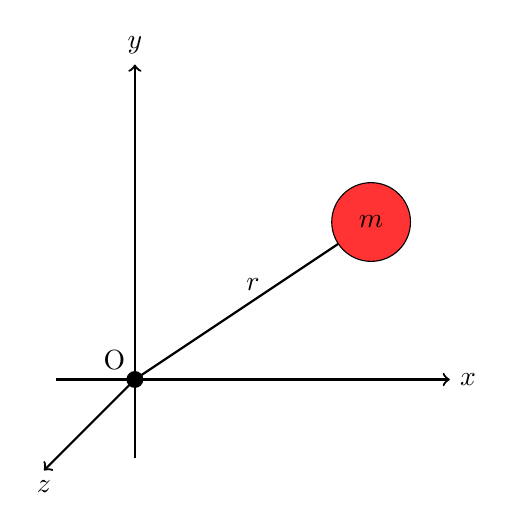
\begin{tikzpicture}

    % Draw the x-axis and y-axis (axes in the plane)
    \draw[thick,->] (-1,0) -- (4,0) node[right] {$x$};
    \draw[thick,->] (0,-1) -- (0,4) node[above] {$y$};

    % Draw the z-axis (out of the plane)
    \draw[thick,->] (0,0) -- (0,0,3) node[below] {$z$};

    % Draw the rod from the origin to the point mass in the xy-plane
    \draw[thick,black] (0,0) -- (3,2) node[midway,above] {$r$};

    % Draw the point mass (red ball) at the end of the rod
    \filldraw[fill=red!80,draw=black] (3,2) circle (0.5) node[] {$m$};

    % Draw the origin
    \filldraw[fill=black] (0,0) circle (0.1) node[above left] {O};

    \end{tikzpicture}
    \subcaption{Physics tells us the moment of inertia for a point mass.}
    \label{fig:MomentofInertiaPointMass}
\end{minipage}%
\hfill
\begin{minipage}{0.5\textwidth} % Right figure (two thirds of the width)
    \centering
    \includegraphics[width=\textwidth]{graphics/Chap03/PlanarAreaWithRectangle4Inertia.png}
    \subcaption{Computing the moment of inertia for a planar area uses Calculus.}
    \label{fig:MomentofInertiaDerivation}
\end{minipage}
\caption{Illustrations of the moment of inertia: (a) for a point mass about the $z$-axis and (b) for a planar area using differential elements. The amazing power of the rectangle is on even fuller display for the computation of the moment of inertia. We want to compute the moment of inertia about the $z$-axis for a continuous body, based on what we know about the moment of inertia of a point mass, $m$, namely, $I_z = m r^2$, where $r$ is the distance of the point mass from the origin.  We apply this knowledge to compute the moment of inertia of the pseudo point mass defined by the differential orange rectangle centered at $(x, y)$, where $\rho \cdot h \cdot dx \cdot dy$ plays the role of a point mass and $\sqrt{x^2 + y^2}$ is the distance from the origin. We use Calculus to sum up the differential inertias along the $y$-direction, yielding a formula for the differntial inertia of a very thin rectangle (its width is $dx$). We use Calculus a second time to add up the inertia associated with each infinitesimally thin rectangle to compute the object's overall moment of inertia. Incredible!}
\label{fig:combinedMomentInertia}
\end{figure}







\subsection{(Optional Read:) Using Again the Power of the Rectangle to Compute the Inertia of a (Planar) Robot Link}
\label{sec:MoementInertiaFirstTime}

This is the first and only time in the textbook that we ``more-or-less'' do a two-dimensional integral. It is perhaps the ultimate illustration of a Superpower of Calculus: adding up Infinitesimal Objects in 2d instead of 1D! Let's get to work. We define the differential mass contained the orange rectangle of Fig.~\ref{fig:MomentofInertiaDerivation} by
\begin{equation}
    dM(x,y) := \rho \cdot h\cdot dy \cdot dx,
\end{equation}
which is density, times thickness, times height, times width. The distance squared of the differential mass from the origin is 
\begin{equation}
    r^2 = x^2 + y^2.
\end{equation}
To compute the differential inertia  $dI_z$ of the entire rectangle of height $(f(x) - g(x))$, we need to do an integral in the $y$-direction, namely
\begin{equation}
    \begin{aligned}
        dI_x &= \int_{g(x)}^{f(x)} r^2 \cdot dM(x, y)  \\
        & = \int_{g(x)}^{f(x)} (x^2 + y^2) \cdot \rho \cdot h\cdot dy \cdot dx ~~\text{(factor out constants)} \\
        & = \rho \cdot h\cdot dx \cdot \int_{g(x)}^{f(x)} (x^2 + y^2) \cdot dy ~~\text{($dx$ is treated as a constant when integrating with respect to $y$)} \\
        &= \rho \cdot h \cdot dx \cdot  (x^2 \cdot y + \frac{1}{3}y^3) \Big|_{g(x)}^{f(x)} ~~\text{(this time, $x$ is treated as a constant when integrating with respect to $y$)} \\
        &= \rho \cdot h\cdot \left[x^2 \cdot \left( f(x) - g(x)\right)   + \frac{1}{3} \cdot \left( f^3(x) - g^3(x)\right) \right] \cdot dx ~~\text{(moved $dx$ to the end)}.
    \end{aligned}
\end{equation}
Wow! That's one big impressive formula for an infinitesimally thin rectangle. Indeed. Now, to get the entire moment of inertia about the $z$-axis, we use Calculus to sum up along the $x$-direction all of the differential moments of inertia, yielding,
\emstat{
\begin{equation}
    I_z = \int_a^b dI_z =  \rho \cdot h\cdot \int_a^b  \left[x^2 \cdot \left( f(x) - g(x)\right)   + \frac{1}{3} \cdot \left( f^3(x) - g^3(x)\right) \right] \,  dx.
\end{equation}
}
The integral can be evaluated in closed form in simple toy examples. However, for most robot links of interest, numerical methods are used to evaluate the integral. QuadGK to the rescue! \\

P.S. We really just did a simple form of two-dimensional integration, a mainstay of Michigan's Math 215 Multivariable Calculus 
    
    
    
    
    
    
    
       
       
       
       
       
       
       
       
       
       
       
       
       
       
     . 




\clearpage

\begin{figure}[hbt]%
\centering
\subfloat[]{%
	\centering
\includegraphics[width=0.5\columnwidth]{graphics/Chap03/AreaBetweenFandGForWasherAndShell.png}}%
\newline
\centering
\subfloat[]{%
%\hspace*{-4cm} 
% \includegraphics[height=0.7\columnwidth, trim={6cm 1cm -1cm 1cm}, clip]
\includegraphics[height=0.5\columnwidth]
{graphics/Chap03/rotateRectangleAboutX.png}}
\hfill
\subfloat[]{%
% %\vspace*{3cm}
% %\hspace*{-4cm} 
% \includegraphics[height=0.7\columnwidth, trim={7cm 1cm -6cm 1cm}, clip]
\includegraphics[height=0.5\columnwidth]{graphics/Chap03/rotateRectangleAboutY01.png}}%
% The trim option takes four lengths, corresponding to the left, bottom, right, and top edges to be trimmed from the image. The syntax for trim is trim={<left> <lower> <right> <upper>}, and you should always use clip alongside trim to ensure the trimming is applied.
    \caption[]{\textbf{Differential volumes, $\bm{dV}$, in the form of disk/washers and shells}. The area upper bounded by $f:[a, b] \to \real$ in blue and lower bounded by $g:[a, b] \to \real$ in red is shown in (a), for $[a, b]=[0, 4]$. The area enclosed is shaded gray. A solid of revolution results by rotating the indicated area about either the $x$-axis or the $y$-axis. Can you visualize it? Through the magic of Calculus, we can compute the volume of the solid of rotation, whether or not we can visualize the resulting solid in our mind. The key point is the following: The Riemann integral comes down to understanding narrow rectangles. Within the area enclosed in (a) is a dark gray ``rectangle'' of width $dx$, the same rectangle we would use to compute the area enclosed by $f$ and $g$. The result of rotating the narrow rectangle about the $x$-axis is the \textbf{washer} shown in (b); a washer is a thin disk with a hole in it, having thickness $dx$. Because its thickness is non-zero, the washer has a small, but non-zero volume, $dV$. The same dark gray rectangle is rotated about the $y$-axis in (c). The blue cylinder is traced out by the right side of the rectangle, and the red cylinder is traced out by the left side of the rectangle. The result is a \textbf{shell}, that is, a cylinder with thickness $dx$. Due to its non-zero thickness, the shell has a small but non-zero volume, $dV$. Calculus tells us how to add up the infinitesimal volumes $dV$ to get the overall volume.}
    \label{fig:introSolidRevolutionAboutXorYaxes}
\end{figure}
\clearpage

\subsection{Solids of Revolution or More on the Power of the Rectangle}


Consider a shape in the plane enclosing a non-zero area, as illustrated in Fig.~\ref{fig:introSolidRevolutionAboutXorYaxes}. A \textbf{solid of revolution} is the result of rotating the shape about either the $x$-axis or the $y$-axis. Can you visualize the two shapes? They are not shown in the Figure. When rotating about the $x$-axis, can you imagine a blue parabolic-shaped vase with a red cone-shaped interior that is laying on its side? Maybe. When rotating about the $y$-axis, can you imagine an upright red cone-shaped object with an anti-parabolic-(square-root)-shaped blue interior? Maybe. To compute the volume of these two shapes, you don't need to be able to sketch them! It's nice if you can sketch the shapes, but that might just confuse you when computing their respective volumes. As shown in Fig.~\ref{fig:introSolidRevolutionAboutXorYaxes}, rotating a rectangle of width $dx$ about the $x$-axis gives a washer (aka, a disk with a hole in the middle) with thickness $dx$, while rotating that same rectangle about the $y$-axis produces a shell, that is, a cylinder with thickness $dx$. Each of these objects has a differential volume equal to $A(x)$ times $dx$. The total volume is then
\begin{empheq}[box=\bluebox]{equation}
\label{eq:SolidRevolutionVtotalEqualsintegralOFdV}
V_{\rm solid} := \int_{a}^{b} dV(x) :=  \int_{a}^{b} A(x) \, dx.    
\end{empheq}
\\

\subsubsection{Computing the Volume}
Without even sketching the solid of revolution that results from rotating the area about an axis, we can understand how to compute its volume. Sounds crazy, right?  The secret is that Riemann Integration is all about narrow rectangles. Rotating a rectangle is much easier to understand than rotating an arbitrary shape. As shown in Fig.~\ref{fig:introSolidRevolutionAboutXorYaxes}, rotating a rectangle of width $dx$ about the $x$-axis gives a washer (aka, a disk with a hole in the middle) with thickness $dx$, while rotating that same rectangle about the $y$-axis produces a shell, that is, a cylinder with thickness $dx$. Each of these objects has a differential volume equal to $A(x)$ times $dx$.
\emstat{
\begin{itemize}
    \item \textbf{Area and Differential Volume of the Disk:} The outer radius is $f(x)$ and the inner radius is $g(x)$, and its thickness is $dx$. Hence, 
    $$A(x) := \pi \left( f^2(x) - g^2(x)\right) \text{ and } dV_{\rm x{\text{-axis}}}:= \pi \left( f^2(x) - g^2(x)\right)\,dx. $$
    \item \textbf{Area and Differential Volume of the Cylinder/Shell:} The top edge of the cylinder/shell is $f(x)$ and its bottom edge is $g(x)$, giving a height of $h:=\left( f(x) - g(x) \right)$. The radius is $r:=x$, and its thickness is $dx$. Because the surface area of a cylinder is $2\pi \cdot r\cdot h$, we have that
    $$A(x) :=2 \,  \pi \, x \left( f(x) - g(x)\right) \text{ and } dV_{\rm y{\text{-axis}}}:= 2\, \pi \, x \left( f(x) - g(x)\right) \,dx. $$
\end{itemize}
}

\bigskip

\begin{propColor}{Volume of a Solid of Revolution}{VolumeSolidRevolution}
\textbf{Key Assumptions:} The area lies totally in the first-quadrant of the $(x, y)$-plane, that is, the quadrant where $x\ge 0$ and $y \ge 0$. Moreover, the area is delimited by two functions $f:[a, b] \to \real$ and $g:[a, b] \to \real$, and for all $0\le a \le x \le b$, $f(x) \ge g(x)$. The last condition means that $f$ is the upper bound on the area, $g$ is the lower bound, and the two functions do not enclose any ``negative area''. \\

Under the above assumptions, the volumes of the two standard solids of revolution are computed as follows:
\begin{align}
\label{eq:Vx}
       V_{\rm x{\text{-axis}}} &:=  \int_a^b  dV_{\rm x{\text{-axis}}} = \int_a^b \pi \left( f^2(x) - g^2(x)\right)\,dx ~~(\text{called the {\bf disc/washer method} for rotation about the $x$-axis})\\[1em]
\label{eq:Vy}
         V_{\rm y{\text{-axis}}} &:=\int_a^b  dV_{\rm y{\text{-axis}}} = \int_a^b 2 \pi \, x \left( f(x) - g(x)\right)\,dx ~~(\text{called the {\bf shell method} for rotation about the $y$-axis}).
\end{align}
The terms disc/washer and shell are defined in Fig.~\ref{fig:introSolidRevolutionAboutXorYaxes} and in the text below.  \\


\end{propColor}

\bigskip

\begin{rem}

On YouTube, there are tons of videos that illustrate these two methods. You need to be careful of two points:
\begin{itemize}
    \item We are applying the disc-washer method to a solid formed by rotating an area about the $x$-axis. If you apply the disc-washer method when rotating the area about the $y$-axis, you will have to use the inverse functions, $x=f^{-1}(y)$ and $x=g^{-1}(y)$. Watch out for this in the videos. Also, what do you do when the inverse functions do not exist? Ouch!
       \item We are applying the shell method to a solid formed by rotating an area about the $y$-axis. If you apply the shell method when rotating the area about the $x$-axis, you will have to use the inverse functions, $x=f^{-1}(y)$ and $x=g^{-1}(y)$. Watch out for this in the videos. Also, what do you do when the inverse functions do not exist? Ouch! You apply our method! 
       \item Our suggestion: do not put yourself in a situation where you need inverse functions; they are typically hard to compute, and their calculation is easily messed up, If you apply the methods as we have presented them, you are good to go. No inverse functions are needed.
       \item \textbf{(Optional Read:) A minor point:} On rare occasions, an area is delimited by $x = F(y)$ and $x = G(y)$, and thus your functions are parameterized by $y$ instead of $x$. This means the roles of the $x$ and $y$ axes have been flipped. In this case, you would draw the dark rectangle as wide in the $x$-direction and short in the $y$-direction, flipping the axes that produce a disc/washer versus a shell. Hence, you have to flip the formulas in \eqref{eq:Vx} and \eqref{eq:Vy} for the disc/washer and shell methods. 
        \item \textbf{(Optional Read:) A minor point:} There are a few videos on YouTube that treat a solid of revolution about an arbitrary axis. Your author has not seen that show up in an engineering course. If it does, you can ask the instructor to teach you how to do it!
\end{itemize}
    
\end{rem}

\bigskip

\emstat{
\textbf{Justification of \eqref{eq:Vx}:} Consider Fig.~\ref{fig:introSolidRevolutionAboutXorYaxes}-(a). When the darkly shaded rectangle of width $dx$ is rotated about the $x$-axis, it traces out the \textbf{washer} shown in Fig.~\ref{fig:introSolidRevolutionAboutXorYaxes}-(b). The outside radius of the washer is $r_2 = f(x)$, the inside radius is $r_1=g(x)$, and its width is $dx$. It follows that the area of the washer is $A(x) = \pi (r_2^2 - r_1^2) = \pi  \left(f^2(x) - g^2(x) \right)$. The washer is the solid of revolution traced out by the small rectangle when it is rotated about the $x$-axis. The \textbf{differential volume} of the washer is its area times width (or thickness), that is, $dV = A(x)\,dx$. Hence, the total volume of the solid of revolution about the $x$-axis is the sum of the differential volumes of revolution. That is, $V = \int_a^b dV = \int_a^b A(x) dx$, we simply add up the differential volumes $dV:=A(x)\,dx$ of each washer from the lower limit of $x$ to its upper limit.\\

    %
    %
\textbf{Justification of \eqref{eq:Vy}:} Consider again Fig.~\ref{fig:introSolidRevolutionAboutXorYaxes}-(a). When the darkly shaded rectangle of width $dx$ is rotated about the $y$-axis, it traces out the \textbf{shell} shown in Fig.~\ref{fig:introSolidRevolutionAboutXorYaxes}-(c).  A ``shell'' is a cylinder with a thin but non-zero thickness; in our case, the thickness is $dx$. The area of the cylinder is $2 \pi \cdot r \cdot h$, where its radius $r = x$ and height $h = f(x) - g(x)$. Therefore, the surface area of the shell is $A(x) = 2 \pi \cdot x \cdot (f(x) - g(x))$, and the differential volume of the resulting solid of revolution is $dV = A(x) \, dx =  2 \pi \cdot x \cdot (f(x) - g(x)) \, dx$.  Hence, the total volume of the solid of revolution about the $y$-axis is the sum of the differential volumes of revolution. That is, $V = \int_a^b dV = \int_a^b A(x) dx$, we simply add up the differential volumes $dV:=A(x)\,dx$ of each shell from the lower limit of $x$ to its upper limit.
}

\begin{example} 
\label{ex:y=SqRootx}
For the two functions $f:[0, 4] \to \real$ by $f(x) = \sqrt{x}$ and $g:[0, 4] \to \real$ by $g(x) = 0.5 x$, compute the volumes for the resulting solids of revolution about the $x$- and $y$-axes. After this example, we'll learn how to sketch the volumes.    
\end{example}

\textbf{Rotation about $x$-axis:}
\begin{lstlisting}[language=Julia,style=mystyle]
# Volume of revolution about the x-axis
using QuadGK

f(x) = sqrt(x)
g(x) = 0.5x
xmin = 0.0
xmax = 4.0

# Area of disc
areaDiscWasher(x) = pi * ( (f(x))^2 - (g(x)^2) )

Volume_x, Error = quadgk(areaDiscWasher, xmin, xmax)
\end{lstlisting}
\textbf{Output} 
\begin{verbatim}
(8.377580409572783, 0.0)
\end{verbatim}

\bigskip

\textbf{Rotation about $y$-axis:}

 \begin{lstlisting}[language=Julia,style=mystyle]
# Volume of revolution about the y-axis
using QuadGK

f(x) = sqrt(x)
g(x) = 0.5x
xmin = 0.0
xmax = 4.0

# Area of disc
areaShell(x) = 2*pi * x* ( f(x) - g(x) )

Volume_y, Error = quadgk(areaShell, xmin, xmax)
\end{lstlisting}
\textbf{Output} 
\begin{verbatim}
(13.40412865472173, 1.244413129087435e-7)
\end{verbatim}

\bigskip

\textbf{Note:} The volumes are not the same. 

\subsubsection{How to Sketch the Volumes}

\emstat{Figure~\ref{fig:sketchingSolidRevolution} walks you through the steps for sketching a solid of revolution about the $x$-axis. The same procedure works for revolving about the $y$-axis. To get the hang of the process, seeing ``live'' examples worked out step-by-step is extremely helpful. \textbf{Recommended Video:} \href{https://youtu.be/4jdZLlibKzo}{Disk Washer Method to Find the Volume of Solids of Revolution} by Quoc Dat Phung, an engineering student in Canada. The video has excellent graphics to support the discussion. The first two examples, which take 10 minutes total at 1X, are adequate to get you going. Quoc Dat uses the term ``antiderivative''. Don't let it bother you; we will cover the concept in an upcoming Chapter. Roughly speaking, it's another term for the ``indefinite integral'' that we covered in Prop.~\ref{thm:IntegralGeneralMonomialProperty}: said another way, the antiderivative of $x^k$ is $\frac{x^{k+1}}{k+1}$. The first two examples worked by Quoc Dat are for rotations about the $x$-axis, and he applies the disk/washer method.
}

\begin{figure}[htb]%`
\centering
\subfloat[]{%
	\centering
\includegraphics[width=0.4\columnwidth]{graphics/Chap03/premirrorImageAboutxAxis.png}}%
\subfloat[]{%
	\centering
\includegraphics[width=0.4\columnwidth]{graphics/Chap03/mirrorImageAboutxAxis.png}}%
\hfill %
\subfloat[]{%
	\centering
\includegraphics[height=0.40\columnwidth]{graphics/Chap03/mirrorImageAboutxAxisInXYZ.png}}%
	\centering
\subfloat[]{%
	\centering
\includegraphics[height=0.40\columnwidth]
{graphics/Chap03/mirrorImageAboutxAxisInXYZwithCircles.png}}%
    \caption[]{\textbf{How to Sketch a Solid of Revolution}. (a) shows the area of interest in the $(x,y)$-plane. To form a rotation about the $x$-axis, make a mirror image of the area below the $x$-axis, as in (b); this is really the area rotated by 180 degrees about the $x$-axis. Next, as in (c), add in a $z$-axis to form a 3D object. The final step is to realize that each point $(x,y)$ in the original area forms a circle in the $(y,z)$-plane when rotated about the $x$-axis. The blue circles in (d) delineate the outer surface of the solid of revolution, and the red circles delineate the inner surface of the solid.}
    \label{fig:sketchingSolidRevolution}
\end{figure}



\begin{figure}[hbt]%
\centering
\subfloat[]{%
	\centering
\hspace*{-2cm} \includegraphics[width=0.6\columnwidth]{graphics/Chap03/yEqxSqRootRevolveAroundXaxis.png}}%
\subfloat[]{%
	\centering
\hspace*{-2cm} \includegraphics[width=0.6\columnwidth]{graphics/Chap03/yEqxSqRootRevolveAroundYaxis.png}}%
    \caption[]{Solids of Revolution for Example~\ref{ex:y=SqRootx} and Fig.\ref{fig:sketchingSolidRevolution} with bounding functions $f:[0, 4]\to \real$ and $g:[0, 4]\to \real$, with $f(x) \ge g(x)$. (a) Rotation of the area about the $x$-axis. (b) Rotation of the area about the $y$-axis. $f$ forms the outer boundary when the area is rotated about the $x$-axis, while it forms the inner boundary when the area is rotated about the $y$-axis. The opposite is true for $g$. }
    \label{fig:solidsRevolutionFequalsSqRtxGequlasZeroPt5x}
\end{figure}


\begin{figure}[hbt]%`
\centering
\subfloat[]{%
	\centering
\includegraphics[width=0.5\columnwidth]{graphics/Chap03/yEqxSqAreaAbove.png}}%
\subfloat[]{%
	\centering
\includegraphics[width=0.5\columnwidth]{graphics/Chap03/yEqxSqRevolveAroundYaxis.png}}%
\hfill %
\subfloat[]{%
	\centering
\includegraphics[width=0.45\columnwidth]{graphics/Chap03/yEqxSqRevolveAroundYaxisWithDisc.png}}%
	\centering
\subfloat[]{%
	\centering
\includegraphics[width=0.45\columnwidth]{graphics/Chap03/yEqxSqRevolveAroundYaxisWithDiscProjected2XZplane.png}}%
    \caption[]{\textbf{Applying the disk/washer method to a solid of revolution about the $\bm{y}$-axis requires} \textcolor{red}{\bf inverse functions}. The area between the line $y=4$ and $y=x^2$ has been shaded in (a). In (b), the shaded area has been rotated around the $y$-axis. This means that each point $(x=f^{-1}(y), y)$ in the shaded area will trace out a circle of radius $f^{-1}(y)$ in the $(x,z)$-plane at a height of $y=f(x)$. In particular, the blue bar in (a), which has thickness $dy$ and radius $r(y) = f^{-1}(y)$, traces out the disk in (c). In (d), the disk has been projected to the $(x, z)$-plane, confirming it is a ``perfect'' circle. Hence, the area in (c) is $A = \pi r^2$, where $r = f^{-1}(y)$. You will be wise to apply the shell method in cases like this one to avoid having to compute inverses of functions. }
    \label{fig:SimpleSolidRevolution}
\end{figure}



\begin{center}
\setlength{\fboxrule}{2pt}  % Setting the thickness of the border line
\fbox{%
  \begin{minipage}{\dimexpr\textwidth-2\fboxrule-2\fboxsep}
    \textcolor{blue}{\bf ChatGPT Prompt for Students:} ``Using the disk/washer method, determine the volume of the solid of revolution formed by rotating about the x-axis the region bounded by $\bm{y = \sqrt{x}}$ and $\bm{y = \frac{1}{2} x}$ for x between zero and four. In addition, using the shell method, determine the volume of the solid of revolution formed by rotating about the y-axis the region bounded by $\bm{y = \sqrt{x}}$ and $\bm{y = \frac{1}{2} x}$ for x from 0 to 4. Provide well-documented Julia code for both methods, explaining each step in its solution. Additionally, generate supporting plots to illustrate the methods explained in the code.''\\
  \end{minipage}
}
\end{center}

\begin{figure}[htb]%`
\centering
\subfloat[]{%
	\centering
\includegraphics[width=0.6\columnwidth]{graphics/Chap03/quarterCircle.png}}%
\subfloat[]{%
	\centering
\includegraphics[width=0.40\columnwidth]{graphics/Chap03/ballbot.png}}%
\caption[]{We can revolve a quarter circle around either axis to form a hemisphere. The volume of a sphere will be twice that of a hemisphere. }
    \label{fig:basketBall}
\end{figure}




\begin{example} \textbf{Volume of a Basketball:} Use the disk/washer method or the shell method to compute the volume of an NBA basketball.     
\end{example}
\textbf{Solution:} According to \href{https://en.wikipedia.org/wiki/Basketball_(ball)}{Wikipedia}, an NBA basketball has a circumference of 75 centimeters (cm), meaning its radius is $r = \frac{75}{2 \pi} = 11.9366$ cm. We'll define $f:[0, r] \to \real$ by $f(x) = \sqrt{r^2 - 1}$ and $g:[0, r] \to \real$ by $g(x) = 0$. The graph of $f$ is a quarter of a circle, as shown in Fig.~\ref{fig:basketBall}. 

\begin{lstlisting}[language=Julia,style=mystyle]
# Volume of revolution about the x-axis
using QuadGK

r = 75/(2*pi)

f(x) = sqrt(r^2 - x^2)
g(x) = 0.0x
xmin = 0
xmax = r

# Area of disc
areaDiscWasher(x) = pi * ( (f(x))^2 - (g(x)^2) )

VolumeSemisphere_x, Error = quadgk(areaDiscWasher, xmin, xmax)

VolumeBasketball = 2 * VolumeSemisphere_x
\end{lstlisting}
\textbf{Output} 
\begin{verbatim}
7124.145724851874
\end{verbatim}

\begin{lstlisting}[language=Julia,style=mystyle]
# Volume of revolution about the y-axis
using QuadGK

r = 75/(2*pi)

f(x) = sqrt(r^2 - x^2)
g(x) = 0.0x
xmin = 0
xmax = r

# Area of disc
areaShell(x) = 2*pi * x* ( f(x) - g(x) )

VolumeSemisphere_y, Error = quadgk(areaShell, xmin, xmax)

VolumeBasketball = 2 * VolumeSemisphere_y
\end{lstlisting}
\textbf{Output} 
\begin{verbatim}
7124.145729241054
\end{verbatim}

\textbf{Our estimate is, therefore, Volume = 7124.145727 cm$\bm{^3}$ $\bm{\pm}$ 4.39e-06}

\Qed.



\textbf{Other Recommended Videos:}
\begin{itemize}

\item \href{https://youtu.be/E6Yh0rli6do}{Cylindrical Shells to Find the Volume of Solids of Revolution} by Quoc Dat Phung has excellent graphics to support what he is teaching. 


\item \href{https://youtu.be/M85_r3pZ5YA}{Disk/Washer vs. Cylindrical Shell...when to use which?} by Quoc Dat Phung has excellent graphics to support what he is teaching. \textbf{Note:} For us, the answer is clear for functions $y=f(x)$ and $y=g(x)$: when rotating about the $x$-axis, use the Disk/Washer Method, and when rotating about the $y$-axis, use the Shell Method. This avoids having to compute inverse functions.

\item \href{https://youtu.be/ydyXf01WNYA}{Disc/Washer Method vs. Shell Method (rotated about different lines)} by \bprp ~has clear, hand-drawn graphics so that you too can make nice sketches.

\item \href{https://youtu.be/cxj0OfZTWEo}{Shell method for volume of revolution (rotated about different axis and lines)} by \bprp ~has clear, hand-drawn graphics so that you too can make nice sketches.

\end{itemize}

\newpage


\begin{figure}[htb]%
\centering
\subfloat[]{%
\includegraphics[width=0.45\columnwidth]{graphics/Chap03/LipschitzExampleA.png}}%
\hfill
\subfloat[]{%
\includegraphics[width=0.45\columnwidth]{graphics/Chap03/LipschitzExampleB.png}}%
\hfill
\caption[]{\textbf{(Lipschitz Continuity)} is more restrictive than ``normal continuity''. You can think of Lipschitz continuity as a rule that puts a bound on how quickly a function can change as you move from one point to another along its graph, forcing the function to behave as if it were ``locally linear''. This means the function doesn’t spike too steeply or drop too suddenly, ensuring a certain smoothness in its graph.}
    \label{fig:LipschitxContinuousFunction}
\end{figure}

\section{(Optional Read:) Proofs Associated with the Chapter}
\label{sec:ProofsChap03}

We open this section by providing proof of the existence of the Riemann-Darboux Integral for functions that satisfy a stronger condition than the ``usual notion of continuity'' as we've used that term so far in the course.

\bigskip

\begin{tcolorbox}[colback=mylightblue, title = {\bf Lipschitz Continuity}, breakable]

\begin{definition}  A function $f:[a, b] \to \real$ is \textbf{Lipschitz continuous} if there exists a finite constant $L < \infty$ such that for all $x, y \in [a, b]$,
\begin{equation}
\label{eq:LipschitzDefinition}
    |f(x) -f(y)| \le L \cdot |x -y|.
\end{equation}
\bigskip

\textbf{Note:} Essentially, Lipschitz continuity means the function cannot grow faster than a linear function with slope $L$. More precisely, for any point $y \in [a, b]$ and all points $x \in [a, b]$
\begin{equation}
\label{eq:LipschitzEquivalentDefinition}
    f(y) - L|x-y| \leq f(x) \leq f(y) + L|x-y|,
\end{equation}    
\end{definition}
as illustrated in Fig.~\ref{fig:LipschitxContinuousFunction}. Near each point $y\in [a, b]$, the local change in $f$ as a function of $x-y$ is linear with slope $L$. Indeed, for $x>y$, $|x-y|=x-y$, and we have $f(x) \le f(y) + L(x-y)$ (a constant plus a slope times the change of $x$ with respect to $y$), while for $x < y$, $|x-y|= -(x-y)$, and we have $f(x) \ge f(y) + L(x-y)$ (one again, a constant plus a slope times the change of $x$ with respect to $y$).
\end{tcolorbox}


\bigskip
\textbf{Note:} From Prop.~\ref{thm:triangleAndReverseTriangleInequality}-(c), the ``no-name property of inequalities'', \eqref{eq:LipschitzDefinition} is equivalent to 
$$-L \cdot |x -y| \le f(x) - f(y) \le L \cdot |x -y|.$$
Adding $f(y)$ to each term gives,
$$f(y) -L \cdot |x -y| \le f(x) \le f(y) + L \cdot |x -y|.$$


\textbf{Note:} Due to the inequality \eqref{eq:LipschitzEquivalentDefinition}, a Lipschitz continuous function cannot have a ``jump'', and hence every Lipschitz continuous function is also ``continuous'' in the sense we have been using the term in this textbook. Indeed, considering Fig.~\ref{fig:ContinuousVsNot}-(b) or -(c), drawing a discontinuous function requires a line with an infinite slope (i.e., a vertical line) or lifting your pen from the paper. In the next Chapter, we'll be more precise about the notion of continuity.
\Qed


\begin{propColor}{(Existence of the Riemann-Darboux Integral for Lipschitz Continuous Functions}{Existence Riemann-DarbouxIntegralLipschitzContinuousFunctions} Suppose that $f:[a, b] \to \real$ is Lipschitz continuous. Then its Riemann-Darboux integral $\int_a^b f(x) \, dx$ exists and is finite.    
\end{propColor}

\textbf{Proof:} We must check the conditions in Definition~\ref{def:RiemannIntegral4ContinuousFunctions} are satisfied. To do that, we recall some of the details. For $a < b$ (finite) real numbers, and $n\ge 1$, define $\Delta x := \frac{b-a}{n}$ and $x_i := a + (i-1) \cdot \Delta x$, for $1 \le i \le n+1$. Then, 
\begin{enumerate}
\renewcommand{\labelenumi}{(\alph{enumi})}
\setlength{\itemsep}{.2cm}
    \item  ${\rm Area}^{\rm Low}_n : = \sum_{i=1}^n h_i^{\rm Low} \cdot \Delta x$, for $h_i^{\rm Low}:= \displaystyle \min_{x \in [x_i, x_{i+1}]} f(x)$ is the \textbf{Riemann lower sum}, and 
     \item  ${\rm Area}^{\rm Up}_n : = \sum_{i=1}^n h_i^{\rm Up} \cdot \Delta x$, for $h_i^{\rm Up}:= \displaystyle \max_{x \in [x_i, x_{i+1}]} f(x)$ is the \textbf{Riemann upper sum}.
\end{enumerate}
We need to show that 
\begin{itemize}
    \item $ \lim_{n \to \infty} {\rm Area}^{\rm Low}_n$ exists and is finite, 
    \item $\lim_{n \to \infty} {\rm Area}^{\rm Up}_n $ exists and is finite, and
    \item the two limits are equal.
\end{itemize}

\textbf{We first show the last property: if the two limits exist and are finite, then they converge to the same value.} \\

The key step is to estimate the max and min of $f:[x_i, x_{i+1}] \to \real$. But from \eqref{eq:LipschitzEquivalentDefinition}, for all $x \in [x_i, x_{i+1}]$
$$    f(x_i) - L |x - x_i| \le f(x), $$
and hence, 
$$h_i^{\rm Low}:=\min_{x \in [x_i, x_{i+1}]} f(x) \ge \min_{x \in [x_i, x_{i+1}]} \left(  f(x_i) - L |x - x_i| \right)  = f(x_i) - L |x_{i+1} - x_i | = f(x_i) - L \Delta x.$$
Similarly, 
from \eqref{eq:LipschitzEquivalentDefinition}, for all $x \in [x_i, x_{i+1}]$
$$    f(x) \le f(x_i) + L |x - x_i|, $$
and hence, 
$$ h_i^{\rm Up}:=\max_{x \in [x_i, x_{i+1}]} f(x) \le \max_{x \in [x_i, x_{i+1}]} \left(  f(x_i) + L |x - x_i| \right)  = f(x_i) + L |x_{i+1} - x_i | = f(x_i) + L \Delta x.$$
In case the math in these steps is unclear, the bounds can be deduced from Fig.~\ref{fig:LipschitxContinuousFunction}.\\

From these inequalities, 
\begin{align*}
     {\rm Area}^{\rm Up}_n - {\rm Area}^{\rm Low}_n &= \sum_{i=1}^n \left(  h_i^{\rm Up}  - h_i^{\rm Low}\right) \Delta x  \\[1em] 
     & \le \sum_{i=1}^n \left(  h_i^{\rm Up}  - h_i^{\rm Low}\right) \Delta x \\[1em]
     &\le \sum_{i=1}^n \left( f(x_i) + L \Delta x  - f(x_i) + L \Delta x \right) \Delta x \\[1em]
     &\le  \sum_{i=1}^n 2  L \Delta x \cdot \Delta x \\[1em]
     &\le n 2 L \left( \frac{b-a}{n} \right)^2 \\[1em]
     &\le 2 L  \frac{(b-a)^2}{n}.
\end{align*}
Hence, 
$$ \lim_{n \to \infty} \left( {\rm Area}^{\rm Up}_n - {\rm Area}^{\rm Low}_n \right) \le  \lim_{n \to \infty}  2 L  \frac{(b-a)^2}{n} = 0.$$
Because ${\rm Area}^{\rm Up}_n - {\rm Area}^{\rm Low}_n \ge 0$, we deduce that
$$ \lim_{n \to \infty}\left({\rm Area}^{\rm Up}_n - {\rm Area}^{\rm Low}_n \right)  = 0,$$
and therefore, if the two limits exist and are finite, then they converge to the same value.\\

To show the convergence of the Riemann Upper or Lower Sum requires a result from Real Analysis that is beyond the scope of this course: the \href{https://en.wikipedia.org/wiki/Monotone_convergence_theorem#:~:text=Informally%2C%20the%20theorems%20state%20that,will%20converge%20to%20the%20infimum.}{Monotone Convergence Theorem}, which is taught in Michigan's Math 451 \textit{Advanced Calculus I}. The theorem states that if a sequence is monotonically increasing and bounded from above, then it has a limit, and the limit is finite; similarly, if a sequence is monotonically decreasing and bounded from below, then it has a limit, and the limit is finite. \\

For us, the sequences of interest are $ {\rm Area}^{\rm Up}_n$ and ${\rm Area}^{\rm Low}_n$, for $n$ a power of two, that is, $n=2^k$.  \textbf{Why Powers of 2?}  When \(n\) is chosen as a power of 2, each step from \(n\) to \(2n\) involves splitting each subinterval into exactly two equal parts. This ensures every new subinterval's maximum cannot exceed the maximum of the ``parent interval'' in the previous partition. To see this, consider a subinterval $[x_i, x_i + \Delta x]$ and divide it into two equal halves, 
$$ [x_i, x_i + \Delta x] = [x_i, x_i + \frac{\Delta x}{2}] ~~ \bigcup ~~ [ x_i + \frac{\Delta x}{2}, x_i + \Delta x]. $$
Then, upon defining, 
\begin{align*}
    h_i^{\rm Up}&:=\max_{x \in [x_i,  x_i + \Delta x]} f(x) \\[1em] 
    \bar{h}_{2i}^{\rm Up}&:=\max_{x \in [x_i, x_i + \frac{\Delta x}{2}]} f(x) \\[1em]
    \bar{h}_{2i+1}^{\rm Up}&:=\max_{x \in [ x_i + \frac{\Delta x}{2}, x_i + \Delta x]} f(x), \\[1em]
\end{align*}
we have that $$h_i^{\rm Up} = \max\{ \bar{h}_{2i}^{\rm Up}, \bar{h}_{2i+1}^{\rm Up} \},$$
and therefore, 
$$h_i^{\rm Up} \cdot  \Delta x \ge  \bar{h}_{2i}^{\rm Up} \cdot \frac{\Delta x}{2} + \bar{h}_{2i+1}^{\rm Up} \cdot \frac{\Delta x}{2},$$
showing that the sequence, ${\rm Area}^{\rm Up}_n$, is monotonically decreasing. Using Lipschitz continuity, we have the sequence is lower bounded by 
$$ \left(f(a) - L|b-a| \right)\cdot (b-a),$$
showing that all of the conditions of the Monotone Convergence Theorem are met.\\

The learner can repeat the above argument with small changes and show that ${\rm Area}^{\rm Low}_n$ is monotonically increasing and bounded from above, and hence also satisfies the conditions of the Monotone Convergence Theorem. 
\Qed

\bigskip


\begin{tcolorbox}[title=\textcolor{black}{Proof of Prop.~\ref{thm:FirstAdditivityProperty} (Additivity Property of the Riemann Integral)}, sharp corners, colback=green!30, colframe=green!80!blue, breakable, fonttitle=\bfseries]

Suppose that $a < b <c$ and $f:[a, c] \to \real$ is continuous. Then the three Riemann Integrals  $\int_{a}^{c} f(x)$, $\int_{a}^{b} f(x)$, and $\int_{b}^{c} f(x)$ all exist and satisfy
$$
%\label{eq:FirstAdditivityProperty}
\int_{a}^{c} f(x) =\int_{a}^{b} f(x) + \int_{b}^{c} f(x).
$$
\end{tcolorbox}


\textbf{Proof:} For many people, Fig.~\ref{fig:RiemannIntegralAdditivity} is proof enough! If we were using the more general Darboux partitions, instead of the uniform partitions $x_i:=a + (i-1)\cdot \Delta x$, then the proof would be immediate as well. Due to our use of simplified partitions, the best way to organize the proof is to wait for the integrability results in Chapter~\ref{sec:WhenRiemannDefiniteIntegral} on piecewise continuous functions, define
\begin{align*}
    f_{ab}(x) &:= f(x), ~ a \le x < b\\
    f_{bc}(x) &:= f(x), ~ b \le x \le c
\end{align*}
and note that $f(x) = f_{ab}(x) + f_{bc}(x)$. Finally, you can then apply Prop.~\ref{thm:SecondAdditivityProperty}.
\Qed

\bigskip


% \begin{tcolorbox}[title=\textcolor{black}{Proof of Prop.~\ref{thm:DummyVariableProperty} (Dummy Variables)}, sharp corners, colback=green!30, colframe=green!80!blue, breakable, fonttitle=\bfseries]

% $$
% %\label{eq:DummyVariableOfIntegration}
%     \int_{a}^{b} f(x) =\int_{a}^{b} f(y) \, dy = \int_{a}^{b} f(\lambda) d\lambda,
% $$
% for any choice of real variables $x, y,$ and $\lambda$. The Riemann Integral depends on the function $f:[a, b] \to \real$ and the lower and upper limits. The integral does not depend on what we name the variable we are plugging into $f$. In other words, the variable under the integral sign is a \textbf{dummy variable}. 

% \end{tcolorbox}



% \bigskip


\begin{tcolorbox}[title=\textcolor{black}{Proof of Prop.~\ref{thm:SecondAdditivityProperty} (Linearity of the Riemann Integral)}, sharp corners, colback=green!30, colframe=green!80!blue, breakable, fonttitle=\bfseries]

Suppose that $a < b$ and each of the functions $1 \le k \le N$, $f_k:[a, b] \to \real$, is Riemann integrable (i.e., their Riemann Integral exists and is finite). Then for constants $\alpha_k \in \real$, the function
$$ f(x):= \alpha_1 \cdot f_1(x) + \alpha_2 \cdot f_2(x) + \cdots + \alpha_N \cdot f_N(x),$$
defined as a ``linear combination of the functions $\{ f_1, f_2, \ldots, f_N\}$'', is Riemann integrable and, moreover, 
$$
    \int_a^b f(x) = \alpha_1 \int_a^b   f_1(x) + \alpha_2 \int_a^b  f_2(x) + \cdots + \alpha_N  \int_a^b f_N(x).
$$   

\end{tcolorbox}


\textbf{Proof:} The proof uses the Riemann Lower and Upper Sums and needs a few key facts that are left to the learner, namely,
\begin{equation}
\label{eq:MaxSumLessSumMaxes}
\begin{aligned}
     \max_{x \in [x_i, x_{i+1}]} \left( \alpha_1 \cdot f_1(x) +  \cdots + \alpha_N \cdot f_N(x)  \right) &\le  \max_{x \in [x_i, x_{i+1}]} \left(\alpha_1 \cdot f_1(x) \right) +  \cdots + \max_{x \in [x_i, x_{i+1}]} \left( \alpha_N \cdot f_N(x) \right)\\
     \\
          \min_{x \in [x_i, x_{i+1}]} \left( \alpha_1 \cdot f_1(x) +  \cdots + \alpha_N \cdot f_N(x)  \right) &\ge  \min_{x \in [x_i, x_{i+1}]} \left(\alpha_1 \cdot f_1(x) \right) +  \cdots + \min_{x \in [x_i, x_{i+1}]} \left( \alpha_N \cdot f_N(x) \right);
\end{aligned}   
\end{equation}
in words, the max of a sum is less than or equal to the sum of the maxes, while the min of a sum is greater than or equal to the sum of the mins.\\

Given, this, we complete the proof. Without loss of generality, we can assume that the coefficients\footnote{If minus signs were involved, then we'd have to deal with $\max~ f(x) = - \min (-f(x))$, etc., making the argument clumsy. In math, whenever possible, we like to reduce things to a simpler case that still shows the result we seek.} $\alpha_k \ge 0$. Indeed, if for some $k$, we have $\alpha_k<0$, then the substitutions $f_k(x) \to -f_k(x)$ and $\alpha_k \to -\alpha_k$ result in the sum being unchanged and all of the coefficients being non-negative. With this condition, it is now true that for all $1 \le k \le n$,
$$ \alpha_k \cdot  \min_{x \in [x_i, x_{i+1}]} f_k(x) = \min_{x \in [x_i, x_{i+1}]} \left(\alpha_k \cdot f_k(x) \right) $$
and
$$ \alpha_k \cdot  \max_{x \in [x_i, x_{i+1}]} f_k(x) = \max_{x \in [x_i, x_{i+1}]} \left(\alpha_k \cdot f_k(x) \right). $$
When combined with \eqref{eq:MaxSumLessSumMaxes}, we have,
\begin{equation}
\label{eq:MaxSumLessSumMaxesPosCoeff}
\begin{aligned}
     \max_{x \in [x_i, x_{i+1}]} \left( \alpha_1 \cdot f_1(x) +  \cdots + \alpha_N \cdot f_N(x)  \right) &\le \alpha_1 \cdot \max_{x \in [x_i, x_{i+1}]}  f_1(x)  +  \cdots +  \alpha_N \cdot \max_{x \in [x_i, x_{i+1}]}f_N(x) \\
     \\
          \min_{x \in [x_i, x_{i+1}]} \left( \alpha_1 \cdot f_1(x) +  \cdots + \alpha_N \cdot f_N(x)  \right) &\ge  \alpha_1 \cdot \min_{x \in [x_i, x_{i+1}]}  f_1(x) +  \cdots + \alpha_N \cdot  \min_{x \in [x_i, x_{i+1}]} f_N(x).
\end{aligned}   
\end{equation}

We now follow our general (simplified) procedure for Riemann Lower and Upper Sums from Chapter~\ref{sec:SimpleRiemannLowerUpperSums}, let $n\ge 2$, and define
\begin{equation}
    \begin{aligned}
        \Delta x&:= \frac{b-a}{n}\\
        x_i&:= a + (i-1)\cdot \Delta x \\
        h_i^{\rm Low} &:=  \min_{x \in [x_i, x_{i+1}]} f(x) \\
        h_i^{\rm Up} &:=  \max_{x \in [x_i, x_{i+1}]} f(x) \\
        h_{i,j}^{\rm Low} &:=  \min_{x \in [x_i, x_{i+1}]} f_j(x) \\
        h_{i,j}^{\rm Up} &:=  \max_{x \in [x_i, x_{i+1}]} f_j(x) \\
    {\rm Area}^{\rm Low}_n &: = \sum_{i=1}^n h_i^{\rm Low} \cdot \Delta x \\
    {\rm Area}^{\rm Up}_n &: = \sum_{i=1}^n h_i^{\rm Up} \cdot \Delta x \\
    {\rm Area}^{\rm Low}_{n,j} &: = \sum_{i=1}^n h_{i,j}^{\rm Low} \cdot \Delta x \\
    {\rm Area}^{\rm Up}_{n,j} &: = \sum_{i=1}^n h_{i,j}^{\rm Up} \cdot \Delta x.
    \end{aligned}
\end{equation}
Then, from \eqref{eq:MaxSumLessSumMaxesPosCoeff}, we have
\begin{equation}
    \sum_{j=1}^N \alpha_j  {\rm Area}^{\rm Low}_{n,j} \le  {\rm Area}^{\rm Low}_n  \le  {\rm Area}^{\rm Up}_n  \le   \sum_{j=1}^N \alpha_j  {\rm Area}^{\rm Up}_{n,j}. 
\end{equation}
Then, because $N$ is finite,
\begin{equation}
    \begin{aligned}
        \lim_{n \to \infty}  \sum_{j=1}^N \alpha_j  {\rm Area}^{\rm Low}_{n,j} &= \sum_{j=1}^N \alpha_j  \lim_{n \to \infty}   {\rm Area}^{\rm Low}_{n,j}\\
         \lim_{n \to \infty}  \sum_{j=1}^N \alpha_j  {\rm Area}^{\rm Up}_{n,j} &= \sum_{j=1}^N \alpha_j  \lim_{n \to \infty}   {\rm Area}^{\rm Up}_{n,j}.
    \end{aligned}
\end{equation}
Because $\{ f_1, \cdots, f_N \}$ are Riemann Integrable, the above limits exist, are finite, and are equal. Hence, by the \href{https://en.wikipedia.org/wiki/Squeeze_theorem#:~:text=The%20squeeze%20theorem%20is%20used,functions%20whose%20limits%20are%20known}{Squeeze Theorem for Limits}, 
$$ \lim_{n \to \infty} {\rm Area}^{\rm Low}_n =\lim_{n \to \infty} {\rm Area}^{\rm Up}_n = \sum_{j=1}^N \alpha_j  \lim_{n \to \infty}   {\rm Area}^{\rm Up}_{n,j} = \sum_{j=1}^N \alpha_j \int_a^b   f_j(x).$$
This proves the result.
\Qed

\begin{tcolorbox}[title=\textcolor{black}{Proof of Cor.~\ref{thm:CorollaryFirstAdditivityProperty} (Generalized First Additivity Property)}, sharp corners, colback=green!30, colframe=green!80!blue, breakable, fonttitle=\bfseries]

For $a$, $b$, and $c$ finite real numbers in no particular order, define $\alpha:= \min\{a, b, c\}$ to be the smallest of the three numbers, and $\beta:= \max\{a, b, c\}$ the largest. If $f:[\alpha, \beta] \to \real$ is continuous, then
\begin{equation}
\label{eq:FirstAdditivityPropertyRearranged02}
    \int_{a}^{b} f(x) = \int_{a}^{c} f(x)~ + \int_{c}^{b} f(x).
\end{equation}    

\end{tcolorbox}

\textbf{Proof:} 

From Prop.~\ref{thm:FirstAdditivityProperty}, if $a < b <c$ and $f:[a, c] \to \real$ is continuous, then the three Riemann Integrals  $\int_{a}^{c} f(x)$, $\int_{a}^{b} f(x)$, and $\int_{b}^{c} f(x)$ all exist and satisfy
$$
    \int_{a}^{c} f(x) =\int_{a}^{b} f(x)~ + \int_{b}^{c} f(x).
$$
Hence,  $\int_{a}^{b} f(x) = \int_{a}^{c} f(x)~ -  \int_{b}^{c} f(x)$.
If we apply \eqref{eq:FlippingOrderLimits} on swapping the order of the limits of the integral, we obtain
$$ \int_{a}^{b} f(x)  =  \int_{a}^{c} f(x)~ +\int_{c}^{b} f(x),$$
which shows the additivity property holds when $c$ is larger than both limits and not just for $c$ between the two limits. \\

Similarly, 
$$  \int_{b}^{c} f(x) = - \int_{a}^{b} f(x)~ + \int_{a}^{c} f(x),$$
by the First (Basic) Additivity Property, and, if we apply \eqref{eq:FlippingOrderLimits}, we obtain
$$ \int_{b}^{c} f(x)  =   \int_{b}^{a} f(x)~ + \int_{a}^{c} f(x),$$
which shows the additivity property holds when $c$ is smaller than both limits. This is half\footnote{The integrals on the left of our three cases all have a lower limit that is smaller than the upper limit. What happens when the reverse is true?} of what we need to show.\\

If we negate the First (Basic) Additivity Property, we obtain,
$$
    -\int_{a}^{c} f(x) = -\int_{a}^{b} f(x)~ - \int_{b}^{c} f(x),
$$
which, upon flipping all three sets of limits of integration, yields
$$
    \int_{c}^{a} f(x) = \int_{b}^{a} f(x)~ + \int_{c}^{b} f(x).
$$
From this, the remaining cases follow easily, and hence, the order of $a$, $b$, and $c$ is immaterial.
\Qed

\bigskip


\begin{tcolorbox}[title=\textcolor{black}{Proof of Prop.~\ref{thm:IntegralShiftProperty} (Shift Property)}, sharp corners, colback=green!30, colframe=green!80!blue, breakable, fonttitle=\bfseries]

Suppose that $a < b$ and $f:[a, b] \to \real$ is continuous and let $x_c \in \real$. Then $g:[a + x_c, b+x_c] \to \real$ by $g(x):=f(x-x_c)$ is also continuous and
$\int_a^b f(x) \, dx = \int_{a+x_c}^{b+x_c} g(x) \, dx$.

\end{tcolorbox}

\bigskip 

A graphical proof is provided by the \href{https://www.khanacademy.org/math/in-in-grade-12-ncert/xd340c21e718214c5:definite-integrals/xd340c21e718214c5:definite-integral-properties/v/definite-integral-shifted-function}{Khan Academy} and in Fig.~\ref{fig:ShitingAndIntegration}. \\


\textbf{Proof:} If you want a formal proof with Riemann Sums, we can develop that too! For simplicity and clarity, we assume the function is monotonically increasing and we use the lower Riemann sum:
\begin{itemize}
    \item $\Delta x := \frac{b-a}{n}$
    \item $x_i = a + (i-1) \Delta x$
      \item ${\rm Area}^{\rm Low}_n : = \sum_{i=1}^n f(x_i) \cdot \Delta x$ is the lower Riemman sum.
\end{itemize}

% We can view this as approximating $f(x)$ by a sum of rectangles, 
% $$f^{\rm Low}_n(x):= \sum_{i=1}^n  f(x_i) \cdot \rect\left( \frac{x - x_{m, i}}{\Delta x} \right),$$
% where the area under $\rect\left( \frac{x - x_{m, i}}{\Delta x} \right)$ equals $\Delta x$.
% Hence, 
% $$\int_a^b f^{\rm Low}_n(x) \, dx = \int_a^b \sum_{i=1}^n  f(x_i) \cdot \rect\left( \frac{x - x_{m, i}}{\Delta x} \right) \, dx = \sum_{i=1}^n \int_a^b f(x_i) \cdot \rect\left( \frac{x - x_{m, i}}{\Delta x} \right) \, dx = \sum_{i=1}^n f(x_i) \Delta x = {\rm Area}^{\rm Low}_n .$$

For $g:[a + x_c, b+x_c] \to \real$ by $g(x):=f(x-x_c)$, we construct its lower Riemann sum, via
\begin{itemize}
    \item $\Delta \bar{x} := \frac{(b+x_c)-(a+x_c)}{n} = \frac{b-a}{n} = \Delta x$
    \item $\bar{x}_i = a + x_c + (i-1) \Delta x = x_i+ x_c$
    \item $ \overline{{\rm Area}}^{\rm Low}_n : = \sum_{i=1}^n g(\bar{x}_i) \cdot \Delta \bar{x} = \sum_{i=1}^n g(x_i + x_c) \cdot \Delta x$ is the lower Riemman sum for $g$.
\end{itemize}

\emstat{Because $g(x_i+x_c):=f(x_i+x_c - x_c) = f(x_i)$, the two lower Riemann sums are identical, and hence, if the integrals exist, they are also identical.}
\Qed
\bigskip


\begin{tcolorbox}[title=\textcolor{black}{Proof of Prop.~\ref{thm:IntegralScalingProperty} (Scaling Property)}, sharp corners, colback=green!30, colframe=green!80!blue, breakable, fonttitle=\bfseries]

Suppose that $a < b$, $f:[a, b] \to \real$ is continuous, and $\omega_0 >0$ is a real number.  Then $g:[\frac{a}{\omega_0}, \frac{b}{\omega_0}] \to \real$ by $g(x):=f(\omega_0 \cdot x)$ is also continuous and
$\int_a^b f(x) = \omega_0 \cdot \int_{\frac{a}{\omega_0}}^{\frac{b}{\omega_0}} g(x)$. 

\end{tcolorbox}

\bigskip
\textbf{Proof:}

We reuse the proof strategy for the Shifting Property. For $g:[\frac{a}{\omega_0}, \frac{b}{\omega_0}]\to \real$ by $g(x):=f(\omega_0 \cdot x)$, we construct its lower Riemann sum, via
\begin{itemize}
    \item $\Delta \bar{x} := \frac{\frac{b}{\omega_0}-\frac{a}{\omega_0}}{n} = \frac{1}{\omega_0} \cdot \frac{b-a}{n} = \frac{1}{\omega_0} \cdot\Delta x$
    \item $\bar{x}_i = \frac{a}{\omega_0} + (i-1) \Delta \bar{x} = \frac{a}{\omega_0} + (i-1) \frac{1}{\omega_0} \cdot\Delta x = \frac{x_i}{\omega_0}$
      \item $ \overline{{\rm Area}}^{\rm Low}_n : = \sum_{i=1}^n g(\bar{x}_i) \cdot \Delta \bar{x} = \sum_{i=1}^n g(\frac{x_i}{\omega_0}) \cdot \frac{1}{\omega_0} \cdot\Delta x$ is the lower Riemman sum for $g$.
\end{itemize}

\emstat{Because $g(\frac{x_i}{\omega_0}):=f(\omega_0 \cdot \frac{x_i}{\omega_0}) = f(x_i)$, the two lower Riemann sums are identical, up to the scale factor of $\frac{1}{\omega_0}$, and hence, if the integrals exist, they are also identical up to the scale factor of $\frac{1}{\omega_0}$.}

For the case $\omega_0 < 0$, the same proof is valid and is not repeated. 
\Qed



\bigskip

\begin{tcolorbox}[title=\textcolor{black}{Proof of Prop.~\ref{thm:TrapezoidalRuleWorks} (Trapezoidal Rule for Computing a Riemann Integral)}, sharp corners, colback=green!30, colframe=green!80!blue, breakable, fonttitle=\bfseries]

Suppose that $a < b$ and $f:[a, b] \to \real$ is continuous. Then the Riemann Integral $\int_{a}^{b} f(x)$ exists and it can be evaluated by the \textbf{Trapezoidal Rule}. That is, 
$$
%\label{eq:TrapezoidalApproxForIntegration}
    \int_{a}^{b} f(x) \, dx= \lim_{n \to \infty}{\rm Area}^{\rm Trap}_n =   \lim_{n \to \infty}  \sum_{i=1}^n \frac{f(x_i) + f(x_{i+1})}{2} \cdot \left(x_{i+1} -x_i\right),
$$ 
where, $\Delta x:=\frac{b-a}{n}$ and $x_i:=a + (i-1) \Delta x$. In the above, the limits mean that for all $\epsilon>0$, there exists $N < \infty$ such that $n \ge N \implies \left| \int_{a}^{b} f(x) \, dx - \sum_{i=1}^n \frac{f(x_i) + f(x_{i+1})}{2} \cdot \left(x_{i+1} -x_i\right) \right| < \epsilon$.

\end{tcolorbox}

\bigskip
\textbf{Proof:} We give the proof for functions that are monotonically increasing. For the general case, one must appeal to the uniform continuity property of continuous functions over closed bounded intervals. \\

If the integral $ \int_{a}^{b} f(x) \, dx$ exists, then the lower and upper Riemann sums for $f$ both exist and converge to the same number, which defines  $\int_{a}^{b} f(x) \, dx$. By Prop.~\ref{thm:LimitLinearCombo}, the average of the lower and upper Riemann sums must also converge to $ \int_{a}^{b} f(x) \, dx$. For monotonic functions, the trapezoidal rule is precisely the average of the upper and lower Riemann sums. Hence, the result is proved.

\Qed.

\bigskip


\begin{tcolorbox}[title=\textcolor{black}{Proof of Prop.~\ref{thm:IntegralsEvenOddFunctions} (Integrals of Even and Odd Functions over Symmetric Intervals)}, sharp corners, colback=green!30, colframe=green!80!blue, breakable, fonttitle=\bfseries]

Suppose that $f:\real \to \real $ is a function and that for $a>0$, the definite integrals  $\int_{-a}^0 f(x) \,dx $ and  $\int_{0}^a f(x)\, dx $ both exist and are finite. Then the following hold:
\begin{enumerate}
\renewcommand{\labelenumi}{(\alph{enumi})}
\setlength{\itemsep}{.2cm}
     \item If $f$ is an even function, 
     \begin{itemize}
         \item  $\int_{-a}^0 f(x)\, dx = \int_{0}^a f(x)\, dx $, and 
         \item  $\int_{-a}^a f(x)\, dx = 2\int_{0}^a f(x)\, dx $.
     \end{itemize}
     \item If $f$ is an odd function, 
     \begin{itemize}
         \item  $\int_{-a}^0 f(x)\, dx = -\int_{0}^a f(x)\, dx $, and 
         \item  $\int_{-a}^a f(x)\, dx = 0$.
     \end{itemize}
     \item For all $[b, c] \subset [-a, a]$,
      \begin{itemize}
         \item  $\int_{b}^c f(x)\, dx = \int_b^c f_e(x)\, dx + \int_b^c f_o(x)\, dx$.
     \end{itemize}
     
      \end{enumerate}

\end{tcolorbox}

\bigskip
\textbf{Proof:} 

\begin{enumerate}
\renewcommand{\labelenumi}{(\alph{enumi})}
\setlength{\itemsep}{.2cm}
     \item If $f$ is an even function, $\int_{-a}^0 f(x)\, dx = \int_{0}^a f(x)\, dx $ follows from Prop.~\ref{thm:IntegralScalingProperty} by taking $\omega_0 = -1$. The second statement is immediate from the first statement.
     
     \item If $f$ is an odd function, $\int_{-a}^0 f(x)\, dx = -\int_{0}^a f(x)\, dx $  follows from Prop.~\ref{thm:IntegralScalingProperty} by taking $\omega_0 = -1$. The second statement is immediate from the first statement.
     
     \item For all $[b, c] \subset [-a, a]$, 
      $\int_{b}^c f(x)\, dx = \int_b^c f_e(x)\, dx + \int_b^c f_o(x)\, dx$
follows from Prop.~\ref{thm:SecondAdditivityProperty} because $f(x) = f_e(x) + f_o(x)$ by the construction of the odd and even parts.
     
      \end{enumerate}
      \Qed

% \bigskip

% \begin{tcolorbox}[title=\textcolor{black}{Proof of Prop.~\ref{thm:VolumeSolidRevolution} (Volume of a Solid of Revolution}, sharp corners, colback=green!30, colframe=green!80!blue, breakable, fonttitle=\bfseries]

% \textbf{Key Assumptions:} The area lies totally in the first-quadrant of the $(x, y)$-plane, that is, the quadrant where $x\ge 0$ and $y \ge 0$. Moreover, the area is delimited by two functions $f:[a, b] \to \real$ and $g:[a, b] \to \real$, and for all $0\le a \le x \le b$, $f(x) \ge g(x)$. The last condition means that $f$ is the upper bound on the area, $g$ is the lower bound, and the two functions do not enclose any ``negative area''. \\

% Under the above assumptions, the volumes of the two standard solids of revolution are computed as follows:
% \begin{align}
% \label{eq:VxProof}
%        V_{\rm x{\text{-axis}}} &:= \int_a^b \pi \left( f^2(x) - g^2(x)\right)\,dx ~~(\text{called the {\bf disc/washer method} for rotation about the $x$-axis})\\[1em]
% \label{eq:VyProof}
%          V_{\rm y{\text{-axis}}} &:= \int_a^b 2 \pi x \cdot \left( f(x) - g(x)\right)\,dx ~~(\text{called the {\bf shell method} for rotation about the $y$-axis}).
% \end{align}
% The terms disc/washer and shell are defined in Fig.~\ref{fig:introSolidRevolutionAboutXorYaxes} and in the text below.  \\
% \end{tcolorbox}



% \bigskip


% \begin{tcolorbox}[title=\textcolor{black}{Proof of Prop.~\ref{thm:ExponentialsAreFast} (Exponentials Grow Faster than any Monomial Function)}, sharp corners, colback=green!30, colframe=green!80!blue, breakable, fonttitle=\bfseries]

% The following limits hold for real variables $x$ and for integers $n$ replacing $x$: 
% \begin{enumerate}
% \renewcommand{\labelenumi}{(\alph{enumi})}
% \setlength{\itemsep}{.2cm}
%     \item For all $a>1$ and integers $0 \le m < \infty$, $\displaystyle{\lim_{x \to \infty}} \frac{a^x}{x^m} = \infty$.
%      \item For all $a > 1$ and integers $0 \le m < \infty$, $\displaystyle{\lim_{x \to \infty}}  \frac{x^m}{a^x} = 0$.
%     \item For all $a > 1$ and integers $0 \le m < \infty$, $\displaystyle{\lim_{x \to \infty}}  {x^m} \cdot {a^x} = \infty$.
% \end{enumerate}

% \end{tcolorbox}

% \bigskip

% \bigskip


% \begin{tcolorbox}[title=\textcolor{black}{Proof of Prop.~\ref{thm:ExponentialsAreFast} (Exponentials Grow Faster than any Monomial Function)}, sharp corners, colback=green!30, colframe=green!80!blue, breakable, fonttitle=\bfseries]

% The following limits hold for real variables $x$ and for integers $n$ replacing $x$: 
% \begin{enumerate}
% \renewcommand{\labelenumi}{(\alph{enumi})}
% \setlength{\itemsep}{.2cm}
%     \item For all $a>1$ and integers $0 \le m < \infty$, $\displaystyle{\lim_{x \to \infty}} \frac{a^x}{x^m} = \infty$.
%      \item For all $a > 1$ and integers $0 \le m < \infty$, $\displaystyle{\lim_{x \to \infty}}  \frac{x^m}{a^x} = 0$.
%     \item For all $a > 1$ and integers $0 \le m < \infty$, $\displaystyle{\lim_{x \to \infty}}  {x^m} \cdot {a^x} = \infty$.
% \end{enumerate}

% \end{tcolorbox}
